%definira klasu dokumenta 
\documentclass[12pt]{report} 

%prostor izmedu naredbi \documentclass i \begin{document} se zove uvod. U njemu se nalaze naredbe koje se odnose na cijeli dokument

%osnovni LaTex ne može riješiti sve probleme, pa se koriste različiti paketi koji olakšavaju izradu željenog dokumenta
\usepackage[croatian]{babel} 
\usepackage{amssymb}
\usepackage{amsmath}
\usepackage{txfonts}
\usepackage{mathdots}
\usepackage{titlesec}
\usepackage{array}
\usepackage{lastpage}
\usepackage{etoolbox}
\usepackage{tabularray}
\usepackage{color, colortbl}
\usepackage{adjustbox}
\usepackage{geometry}
\usepackage[classicReIm]{kpfonts}
\usepackage{hyperref}
\usepackage{fancyhdr}
\usepackage{verbatim}
\usepackage{hyperref}

\usepackage{float}
\usepackage{setspace}
\restylefloat{table}


\patchcmd{\chapter}{\thispagestyle{plain}}{\thispagestyle{fancy}}{}{} %redefiniranje stila stranice u paketu fancyhdr

%oblik naslova poglavlja
\titleformat{\chapter}{\normalfont\huge\bfseries}{\thechapter.}{20pt}{\Huge}
\titlespacing{\chapter}{0pt}{0pt}{40pt}


\linespread{1.3} %razmak između redaka

\geometry{a4paper, left=1in, top=1in,}  %oblik stranice

\hypersetup{ colorlinks, citecolor=black, filecolor=black, linkcolor=black,	urlcolor=black }   %izgled poveznice


%prored smanjen između redaka u nabrajanjima i popisima
\newenvironment{packed_enum}{
	\begin{enumerate}
		\setlength{\itemsep}{0pt}
		\setlength{\parskip}{0pt}
		\setlength{\parsep}{0pt}
	}{\end{enumerate}}

\newenvironment{packed_item}{
	\begin{itemize}
		\setlength{\itemsep}{0pt}
		\setlength{\parskip}{0pt}
		\setlength{\parsep}{0pt}
	}{\end{itemize}}




%boja za privatni i udaljeni kljuc u tablicama
\definecolor{LightBlue}{rgb}{0.9,0.9,1}
\definecolor{LightGreen}{rgb}{0.9,1,0.9}
\definecolor{LightTeal}{rgb}{0.9,0.95,0.95}
\definecolor{LightRed}{rgb}{1,0.9,0.9}

%Promjena teksta za dugačke tablice
\DefTblrTemplate{contfoot-text}{normal}{Nastavljeno na idućoj stranici}
\SetTblrTemplate{contfoot-text}{normal}
\DefTblrTemplate{conthead-text}{normal}{(Nastavljeno)}
\SetTblrTemplate{conthead-text}{normal}
\DefTblrTemplate{middlehead,lasthead}{normal}{Nastavljeno od prethodne stranice}
\SetTblrTemplate{middlehead,lasthead}{normal}

%podesavanje zaglavlja i podnožja

\pagestyle{fancy}
\lhead{Programsko inženjerstvo}
\rhead{TrueBlood}
\lfoot{MEGATRON}
\cfoot{stranica \thepage/\pageref{LastPage}}
\rfoot{\today}
\renewcommand{\headrulewidth}{0.2pt}
\renewcommand{\footrulewidth}{0.2pt}


\begin{document} 
	
	
	
	\begin{titlepage}
		\begin{center}
			\vspace*{\stretch{1.0}} %u kombinaciji s ostalim \vspace naredbama definira razmak između redaka teksta
			\LARGE Programsko inženjerstvo\\
			\large Ak. god. 2021./2022.\\
			
			\vspace*{\stretch{3.0}}
			
			\huge TrueBlood\\
			\Large Dokumentacija, Rev. \textit{1}\\
			
			\vspace*{\stretch{12.0}}
			\normalsize
			Grupa: \textit{MEGATRON}\\
			Voditelj: \textit{Toni Ivanković}\\
			
			
			\vspace*{\stretch{1.0}}
			Datum predaje: \textit{19. studenoga 2021.}\\
	
			\vspace*{\stretch{4.0}}
			
			Nastavnik: \textit{Ivan Lovrić}\\
		
		\end{center}

	
	\end{titlepage}

	
	\tableofcontents


	
\chapter{Dnevnik promjena dokumentacije}
		
	%	\textbf{\textit{Kontinuirano osvježavanje}}\\
				
		
		\begin{longtblr}[
				caption = {Dnevnik promjena dokumentacije},
				label=none
			]{
				width = \textwidth, 
				colspec={|X[2]|X[13]|X[3]|X[3]|}, 
				rowhead = 1
			}
			\hline
			\textbf{Rev.}	& \textbf{Opis promjene/dodatka} & \textbf{Autori} & \textbf{Datum}\\[3pt] \hline
			0.1 & Napravljen predložak.	& Toni & 28.10.2021. 		\\[3pt] \hline 
        	0.2 & Započeto pisanje opisa projektnog zadatka & Toni & 3.11.2021. \\[3pt] \hline 
        	0.3 & Napravljeni inicijalni dijagrami obrazaca uporabe & Toni & 4.11.2021. \\[3pt] \hline
        	0.4 & Popravljeni dijagrami obrazaca uporabe, dodani sekvencijski dijagrami & Toni & 6.11.2021. \\[3pt] \hline
        	0.5 & Dodani opisi dijagrama obrazaca uporabe & Toni & 7.11.2021. \\[3pt] \hline
        	0.6 & Započeto pisanje poglavlja o arhitekturi sustava & Jakov, Luka & 12.11.2021. \\[3pt] \hline
        	0.7 & Uređivanje dosadašnjeg dokumenta, razrada ostalih zahtjeva & Toni & 14.11.2021. \\[3pt] \hline
        	0.8 & Dovršen opis projektnog zadatka, dodane reference među dijelovima dokumenta, dodan dnevnik sastajanja & Toni & 16.11.2021. \\[3pt] \hline
        	0.9 & Dodani dnevnici sastajanja u Dodatak (1-5) & Dora & 16.11.2021. \\[3pt] \hline
        	0.10 & Preuređeni opisi UC 1-8, izmijenjeni UC na dijagramu \textit{Uređivanje postojećih računa} & Toni & 17.11.2021. \\[3pt] \hline
        	0.11 & Preuređeni opisi UC 8-15, dodan UC 3.1, izmijenjeni UC na dijagramu, napisani rizici u sustavu i opcionalne funkcionalnosti u poglavlju 2.5 i 2.7 & Toni & 18.11.2021. \\[3pt] \hline
        	0.12 & Dodani dnevnici sastajanja (6-7) & Dora & 18.11.2021. \\[3pt] \hline
        	0.13 & Popravljeno poglavlje Arhitektura po komentarima mentora (model i opisi te same tablice baze podataka) & Jakov & 19.11.2021. \\[3pt] \hline
        	0.14 & Dodano poglavlje 4.1. Baza podataka, detaljnije opisano poglavlje 2.3 Odabir tehnologije & Ana & 19.11.2021. \\[3pt] \hline
        	0.15 & Preuređen UC3.1 & Marko & 19.11.2021. \\[3pt] \hline
        	0.16 & Dodano poglavlje 4.2. Dijagram razreda & Jakov & 19.11.2021. \\[3pt] \hline
        	1.0 & Uređena tablica aktivnosti & Toni, Jakov, Ana, Luka, Marko, Borna, Dora & 19.11.2021. \\[3pt] \hline
		\end{longtblr}
	
	
		%\textit{Moraju postojati glavne revizije dokumenata 1.0 i 2.0 na kraju prvog i drugog ciklusa. Između tih revizija mogu postojati manje revizije već prema tome kako se dokument bude nadopunjavao. Očekuje se da nakon svake značajnije promjene (dodatka, izmjene, uklanjanja dijelova teksta i popratnih grafičkih sadržaja) dokumenta se to zabilježi kao revizija. Npr., revizije unutar prvog ciklusa će imati oznake 0.1, 0.2, …, 0.9, 0.10, 0.11.. sve do konačne revizije prvog ciklusa 1.0. U drugom ciklusu se nastavlja s revizijama 1.1, 1.2, itd.}
	

	\chapter{Opis projektnog zadatka}
	
	

\begin{comment}

		\textbf{\textit{dio 1. revizije}}\\
        		
		\textit{Na osnovi projektnog zadatka detaljno opisati korisničke zahtjeve. Što jasnije opisati cilj projektnog zadatka, razraditi problematiku zadatka, dodati nove aspekte problema i potencijalnih rješenja. Očekuje se minimalno 3, a poželjno 4-5 stranica opisa.	Teme koje treba dodatno razraditi u ovom poglavlju su:}
		\begin{packed_item}
			\item \textit{potencijalna korist ovog projekta}
			\item \textit{postojeća slična rješenja (istražiti i ukratko opisati razlike u odnosu na zadani zadatak). Dodajte slike koja predočavaju slična rješenja.}
			\item \textit{skup korisnika koji bi mogao biti zainteresiran za ostvareno rješenje.}
			\item \textit{mogućnost prilagodbe rješenja }
			\item \textit{opseg projektnog zadatka}
			\item \textit{moguće nadogradnje projektnog zadatka}
		\end{packed_item}
		
		\textit{Za pomoć pogledati reference navedene u poglavlju „Popis literature“, a po potrebi konzultirati sadržaj na internetu koji nudi dobre smjernice u tom pogledu.}
		\eject

\end{comment}

		\section{Cilj projekta i domena primjene}
        \par{Cilj projekta TrueBlood je napraviti programsku potporu te korisničko sučelje za sustav dobrovoljnog darivanja krvi. Web aplikacija nudi mogućnost stvaranja korisničkih računa za darivatelje (donore), evidenciju pokušaja doniranja krvi, evidenciju trenutnih zaliha krvi, i mnoge druge funkcionalnosti koje su opisane u nastavku. Svrha aplikacije je obogatiti iskustvo darivanja te potaknuti ljude da na jednostavniji način pristupe procesu i dobrim djelom pomognu opterećenom zdravstvenom sustavu. Aplikacija velik dio funkcionalnosti radi automatski, pa se time rasterećuje osoblje i ubrzava i poboljšava cjelokupni proces.}
        \par{
        S obzirom na domenu u kojoj se ova aplikacija može primijeniti, potencijalni zainteresirani naručitelji bili bi zavod za javno zdravstvo, ministarstvo zdravstva, Crveni križ, ili slična institucija koja se masovno bavi transfuzijskom medicinom te ima potrebu za automatizacijom procesa darivanja krvi i održavanja stanja zaliha krvi.
        }
        
        \section{Postojeća rješenja}
        
        \par {Dio funkcionalnosti koje razvijamo u ovom projektu već postoji u sustavu Hrvatskog zavoda za transfuzijsku medicinu (\url{https://www.hztm.hr}), gdje je također moguće vidjeti trenutne zalihe krvi u odnosu na optimalne razine, a sustav ispisuje i upozorenje o nedostatku pojedinih krvnih grupa. S druge strane, sustav HZTM-a ne nudi funkcionalnost opisanu u našem zadatku, gdje se donori mogu sami prijaviti u sustav te imati uvid u svoje prethodne pokušaje darivanja, a ne nudi ni slanje potvrda mailom ni naknadno ispisivanje potvrda. Ipak, sustav HZTM-a poslužio nam je kao dobra baza iz koje smo mogli vidjeti dosadašnju realizaciju bar dijela sustava.\\}
        
        
        \begin{figure}[H]
			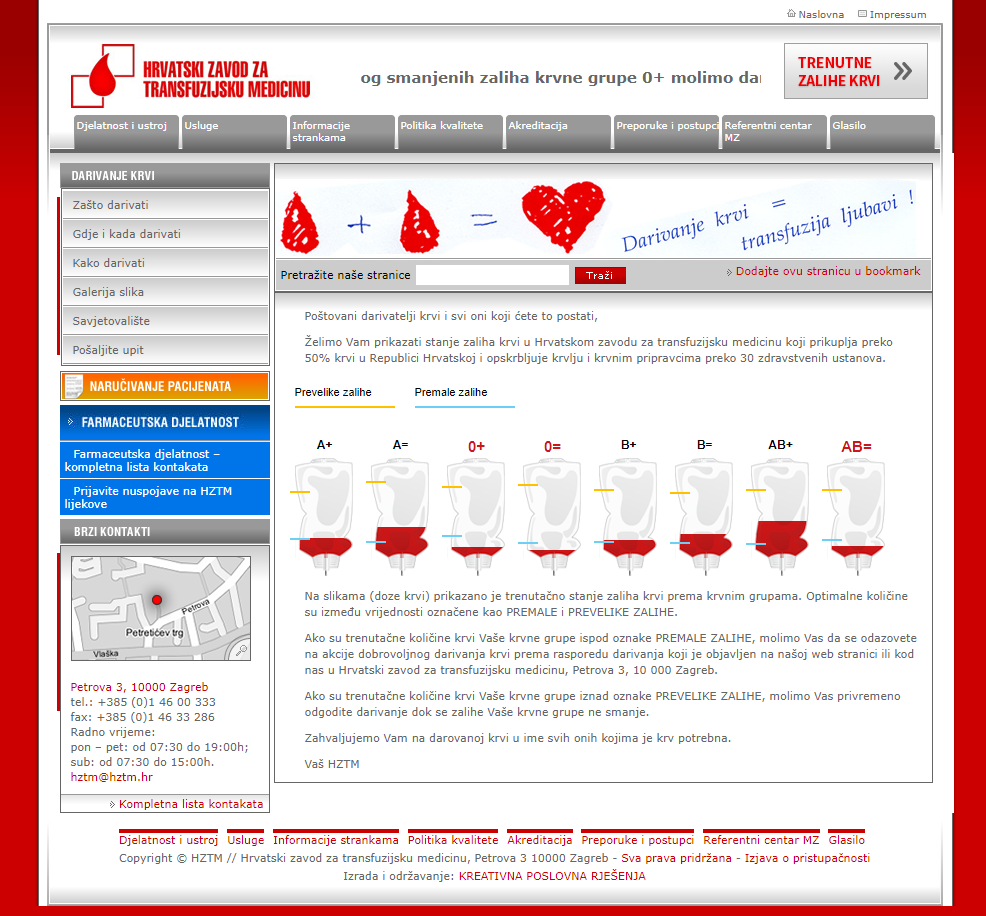
\includegraphics[scale=0.6]{slike/hztm-stranica.PNG}
			\centering
			\caption{Postojeća stranica HZTM-a}
			\label{fig:hztm-stranica}
		\end{figure}
        
        \section{Odabir tehnologije}
        
            \par {Aplikacija je izrađena u razvojnom okviru\textit{ Java Spring Boot} s poslužiteljske strane, a u \textit{Reactu} sa klijentske strane. Za pohranu, organizaciju i pristup podacima sustav koristi PostgreSQL bazu podataka pokrenutu u Docker spremniku. Aplikacija je puštena u pogon preko javno dostupne cloud platforme Heroku. Navedeni razvojni okviri nude sve funkcionalnosti potrebne za izradu opisanog sustava, što će biti detaljnije opisano u poglavlju \ref{arhitektura} i u drugoj reviziji u poglavlju \textit{Implementacija}. \\}
            %Umetnuti referencu u 2. ciklusu
            
        \section{Detaljan opis sustava}
        
            \par{
            Aplikaciji mogu pristupiti i prijavljeni i neprijavljeni korisnici koji imaju različite ovlasti u sustavu.
            \\
            Neprijavljeni korisnici imaju uvid u trenutne razine zaliha krvi i mogućnost prijaviti se ili se registrirati te time steći ovlasti prijavljenog korisnika.
            \\
            Prijavljeni korisnici po razini ovlasti dijele se na donore, djelatnike banke i administratore.
            }
             \par{
            Donori se mogu registrirati samostalno i prije darivanja krvi na javnoj stranici aplikacije. Ako im račun pak stvori djelatnik banke na prvom darivanju krvi, donori ne moraju prolaziti kroz proces registracije, već se prijavljuju s postojećim podatcima. 
            }
             \par{
            U svakom slučaju, pri stvaranju bilo kojeg računa u sustavu na e-adresu šalje se poruka s generiranim identifikatorom, inicijalnom lozinkom i poveznicom za aktivaciju. Nakon pristupa poveznici za aktivaciju, račun je aktiviran i može se koristiti.
            }
             \par{
            Nakon prijave u sustav, donori imaju pristup svim prošlim pokušajima darivanja krvi, imaju uvid u trenutno stanje zalihe njihove krvne grupe i imaju mogućnost izmijeniti neki od matičnih ili kontakt podataka svog računa (kao npr. adresu, broj telefona, e-adresu i sl.). Donori ne mogu mijenjati zdravstvene podatke računa, kao što su krvna grupa i trajno odbijanje. Donorima se također nudi mogućnost preuzimanja potvrde o bilo kojem prijašnjem darivanju krvi.
            }
             \par{Djelatnici banke prijavom u sustav mogu mijenjati svoje matične i kontakt podatke, uređivati sve podatke donora, evidentirati slanje određenog broja doza krvi u vanjsku instituciju (bolnicu) te evidentirati novi pokušaj darivanja krvi. Pri evidenciji pokušaja darivanja, koji se tipično radi na akciji darivanja krvi, djelatnik banke evidentira potrebne zdravstvene podatke kao i uspješnost pokušaja darivanja te, ukoliko zabilježeni podatci sadrže neke od podataka koji to impliciraju, evidentira trajno odbijanje donora u njegovom računu.
            }
            \par{
            Administratori sustava u sustavu imaju ovlast kreirati nove račune djelatnika banke, deaktivirati bilo koji račun u sustavu (u slučaju pogrešnog stvaranja, smrti ili prekida radnog odnosa) te definirati optimalne razine zaliha krvi za svaku krvnu grupu. Optimalne razine služe svim korisnicima sustava da jednostavnije zaključe značenje trenutnih zaliha krvi. Optimalne granice također služe i za okidanje slanja upozorenja korisnicima sustava. 
            }
            \par{
            Kada razina zalihe krvi pojedine krvne grupe padne ispod donje optimalne granice, svi djelatnici banke u sustavu dobivaju upozorenje o tome, a upozorenje dobivaju i zabilježeni donori te krvne grupe.\\
            Upozorenje se izdaje i prijelazom gornje optimalne granice, ali samo djelatnicima banke. \\
            Donori pak dodatnu obavijest dobivaju kada istekne njihov period zabrane darivanja. Naime, iz zdravstvenih razloga, donori ne smiju prečesto darivati krv, pa za muškarce minimalni period između dva darivanja krvi iznosi tri mjeseca, a za žene četiri mjeseca. Kako donori ne bi zaboravili na istek tog perioda zabrane, sustav im po isteku tog perioda šalje obavijest.
            }
            \par{
            S obzirom na to da se pri stvaranju bilo kojeg računa lozinka generira automatski, svi prijavljeni korisnici sustava imaju mogućnost promijeniti svoju lozinku u nešto što će lakše zapamtiti.
            }
        
        \section{Prepoznati i razriješeni rizici}
            \par{
            Mnogi rizici u radu sustava i njegovom korištenju prepoznati su unaprijed i razriješeni. Neki rizici proizlaze iz domene primjene, a neki iz predviđanja nesavršenog ponašanja u radu sa sustavom. Neki od prepoznatih rizika i njihova implementirana rješenja ili razlozi odbacivanja su:
            }
            \begin{itemize}
                \item Korisnik sustava zaboravlja svoj userId (donorId, bankworkerId) iako već ima stvoren račun
                \begin{itemize}
                    \item U e-poruci s poveznicom za aktivaciju navedeni su i donorId i inicijalna lozinka, pa se korisnik pronalaskom aktivacijske poruke može podsjetiti zaboravljenih podataka
                    \item Djelatnik banke donora i administrator djelatnika banke može pretražiti po bilo kojoj kombinaciji podataka, npr. imena, prezimena ili OIB-a. Na taj način može se pronaći račun u sustavu i podsjetiti donorIdja.
                \end{itemize}
                
                \item Donor pri stvaranju računa nema neki podatak
                \begin{itemize}
                    \item Kao obavezni podatci označeni su samo oni koje bi većina ljudi trebala znati ili imati uvijek dostupno
                    \item Ako donor račun stvara samostalno, uvijek može odgoditi stvaranje računa dok ne pronađe obavezni podatak koji mu nedostaje
                    \item Neobavezni podatci ne moraju se unijeti pri stvaranju računa pa ih donor može unijeti i kasnije prijavom u sustav, ili pri idućem doniranju
                \end{itemize}
                
                \item Podatci koji se unesu za donora mogu zabunom biti semantički neispravni (tipfeleri pri unosu adrese, broja telefona, ...) što validacija sustava ne može prepoznati
                \begin{itemize}
                    \item Pri svakom doniranju, djelatnik banke provjerava unesene podatke s donorom te ih popravlja u slučaju greške
                    \item Donor pogrešne podatke može i samostalno ispraviti prijavom u sustav i pregledom osobnih podataka
                \end{itemize}
                
                \item Sustav se može zablokirati zbog neadekvatnog sklopovlja pa se neke aktivnosti ne mogu pravovremeno obaviti
                \begin{itemize}
                    \item U ovakvom ekstremnom slučaju može se ručno voditi evidencija podataka koji su neophodni za obaviti trenutno dok se problem ne riješi pa se podatci unesu naknadno, a aktivnosti koje nije nužno obaviti u istom trenutk mogu se odgoditi do oporavka sustava
                \end{itemize}
                
                \item Baza podataka pri pokušaju unosa nema dovoljno prostora za pohranu novih zapisa
                \begin{itemize}
                    \item Sustav je dovoljno malen da ovo odstupanje ne predstavlja značajan rizik
                    \item Administrator sustava mogao bi s vremena na vrijeme voditi računa o popunjenosti diska s bazom podataka i tako na vrijeme spriječiti nastanak opisane situacije
                    \item Rizik se može na vrijeme spriječiti većom investicijom u opremu
                \end{itemize}
                
                \item Neovlašteni korisnik može nasumično pogoditi aktivacijsku poveznicu i aktivirati račun bez dopuštenja
                \begin{itemize}
                    \item Aktivacijska poveznica dovoljno je dugačka da ovo ne predstavlja značajan rizik
                \end{itemize} 
                
                \item Djelatnik banke želi promijeniti donorId nekog donora, a donorId je primarni ključ u bazi podataka (isto vrijedi i za odnos administrator - djelatnik banke)
                \begin{itemize}
                    \item Primarni ključevi samo se ispisuju na ekran pri pregledu i uređivanju podataka računa i ne mogu se mijenjati.
                    \item Nije prepoznata funkcionalno nužna situacija kada bi ova funkcionalnost bila potrebna, osim iz \textit{estetskih} razloga 
                \end{itemize}
                
                \item Djelatnik banke na doniranju pogrešno tumači neki zdravstveni podatak i pogrešno evidentira trajno odbijanje donora koji ne bi trebao biti trajno odbijen
                \begin{itemize}
                    \item Trajno odbijanje, kao i ostali podatci, može se naknadno ispraviti u sustavu ako se ispostavi da je riječ o pogrešci
                \end{itemize}
                
                \item Donor prešućuje neki od podataka zbog kojih ne bi trebao moći darivati krv
                \begin{itemize}
                    \item Sustav nikako ne može otkriti ovu informaciju, već je ovo problem iz domene primjene (koji je većinom riješen time da se doniranje krvi ne plaća i da se ampula krvi dodatno testira na krvnu grupu i patogene)
                \end{itemize}
                
            \end{itemize}
        
        
        \section{Ograničenja u implementaciji}
            
            \par{
            S obzirom na ograničen vremenski rok i ograničene resurse za izradu sustava, na brojnim mjestima u dogovoru s asistentom dogovoren je nužan i dovoljan opseg rješenja. Taj opseg definiran je funkcionalnim i nefunkcionalnim zahtjevima, dok su dodatne stvari ostavljene na slobodu timu za implementaciju.
            }
            \par{
            Dio problema sa sustavom proizlazi iz ograničenih resursa dostupnih za puštanje aplikacije u pogon na besplatnom servisu \textit{Heroku}, koji gasi aplikaciju nakon određenog vremena u kojemu ne primi nijedan zahtjev. Zbog toga neke funkcionalnosti (poput slanja obavijesti o ponovnoj mogućnosti darivanja) neće raditi pouzdano. Kako bi se ove funkcionalnosti ispitale treba prvo napraviti neki zahtjev i na klijentski poslužitelj i na poslužitelj poslužiteljske aplikacije kako bi se oni pokrenuli, a nakon toga u redovnom korištenju aplikacije ne bi trebalo biti problema. Kako se obavijest o ponovnoj mogućnosti darivanja šalje svaki dan u 12:00 za sve donore koji su donirali krv tri/četiri mjeseca ranije, radi ispitivanja potrebno je netom prije 12:00 poslati bilo kakav zahtjev poslužiteljskoj aplikaciji kako bi se ona pokrenula (i naravno, imati donora u sustavu kojemu na taj dan istječe period nemogućnosti darivanja).
            }
            \par{
            Potencijalan problem predstavlja i servis e-pošte, koji u nekom trenutku može onemogućiti korištenje njegovih usluga zbog sigurnosnih razloga (previše poruka i slično). Oba problema bila bi riješena posjedovanjem vlastitog poslužitelja koji bi aplikaciju držao stalno upaljenom i na kojemu bi se mogao pokrenuti vlastiti servis za e-poruke.
            }
            \par{
            Pri izradi sustava razmatrane su brojne dodatne i alternativne mogućnosti i scenariji koji u ovoj inačici aplikacije nisu podržane. Takve mogućnosti dokumentirane su u sljedećem odjeljku pa se u nekoj od budućih implementacija sustav može nadograditi da podržava neke od navedenih alternativnih mogućnosti. Te mogućnosti najčešće uključuju mogućnosti koje bi olakšale korisnicima korištenje sustava i dale dodatne funkcionalnosti koje se trenutno mogu izvoditi zaobilazno ili se zasad uopće ne mogu izvodti.
            }
        
        \section{Mogućnosti za nadogradnju}
            \par{
            S obzirom na prepoznate rizike vezane za olakšanje korištenja sustava i izvođenje dosad nemogućih radnji, osmišljene su sljedeće mogućnosti za buduću nadogradnju:
            \begin{itemize}
            
                 \item Korisnik sustava pri stvaranju računa ima zabilježenu pogrešnu e-adresu pa ne dobije poruku s aktivacijskom poveznicom, a novi račun ne može stvoriti jer su u sustavu već zabilježeni podatci koji moraju biti jedinstveni 
                 \\ ILI
                \\ Korisnik je zagubio poruku s aktivacijskom poveznicom i donorId-jem prije aktivacije računa (ili ju nije primio zbog prepunjene memorije pretinca e-pošte)
                \begin{itemize}
                    \item Moguća je nadogradnja koja  bi djelatniku banke / administratoru pri pregledu računa donora/djelatnika ostavila mogućnost ponovnog slanja poruke s aktivacijskom poveznicom uz eventualni ispravak e-adrese
                    \item Moguća je nadogradnja koja bi ostavila mogućnost stvaranja novog računa s istim podatcima sve dok se račun ne aktivira te bi se neaktivirani račun s istim podatcima automatski obrisao
                \end{itemize}
                
                 \item Korisnik sustava želi ostati prijavljen odmah po otvaranju aktivacijske poveznice, bez ponovnog upisa podataka za prijavu
                \begin{itemize}
                    \item Iako je ovo samo jednokratno produljenje procesa koje ne utječe značajno na iskustvo korisnika (koji, ako ima aktivacijsku poveznicu, sigurno ima i podatke za prijavu jer se nalaze u istoj poruci), moguća je nadogradnja koja bi stvorila sjednicu korisnika odmah nakon pristupa poveznici za aktivaciju
                \end{itemize}
                
                 \item Administrator zabunom deaktivira račun nekog korisnika sustava
                \begin{itemize}
                    \item Moguća je nadogradnja koja bi administratoru omogućila reaktivaciju nekog računa u sustavu
                \end{itemize}
                
                \item Donor svoju krvnu grupu može ne znati unaprijed, a u sustavu je pretpostavljeno da se podatak može odmah otkriti iako je uobičajena praksa da se krv testira naknadno
                \begin{itemize}
                    \item Krvna grupa može ostati nepopunjena pa se popuniti nakon što se obavi test na bilo koji način
                \end{itemize}
                
                \item Doza krvi na serološkom testiranju može završiti kao nepovoljna i mora se odbaciti
                \begin{itemize}
                    \item Moguća je nadogradnja gdje bi u sustavu postojala i evidencija pojedinih doza krvi koje se onda mogu evidentirati kao nepovoljne i povezati s donorima
                    \item Trenutno moguće rješenje je vođenje evidencije o dozama van sustava i ručno povezivanje s donorima
                \end{itemize}
                
                \item Administrator nije definirao optimalne granice zaliha pa stanje zaliha ne prikazuje podatke koji vizualno imaju korisno značenje
                \begin{itemize}
                    \item Moguća je nadogradnja u kojoj bi sustav administratoru slao upozorenja dok ne definira granice
                \end{itemize}
                
                \item Korisnik sustava zaboravio je lozinku pa ne može pristupiti računu
                \begin{itemize}
                    \item Moguća je nadogradnja koja bi, u slučaju promijenjene lozinke koja se ne može pronaći u e-poruci s aktivacijskom poveznicom, omogućila promjenu lozinke putem e-adrese koja je navedena u računu ili slanje postojeće lozinke na tu e-adresu  
                \end{itemize}
                
                \item Donor želi potvrdu o doniranju poslanu na e-adresu umjesto preuzimanja
                \begin{itemize}
                    \item Moguća je nadogradnja koja bi uz preuzimanje ponudila i mogućnost slanja potvrde na e-adresu, vrlo slično aktivnosti opisanoj u koraku 8 obrasca uporabe \hyperref[UC6]{UC6}
                \end{itemize}
                
                \item Donor želi potvrdu o doniranju i za neuspješan pokušaj doniranja
                \begin{itemize}
                    \item Moguća je nadogradnja koja bi omogućila generiranje PDF potvrde za sve pokušaje doniranja, ne samo za uspješne
                \end{itemize}
                
                \item U sustavu je zabilježena pogrešna e-adresa donora na koju će se slati poruka s aktivacijskom poveznicom i PDF potvrde o doniranjima
                \begin{itemize}
                    \item PDF potvrda ne sadrži nikakve osjetljive podatke pa ona ne predstavlja značajan rizik za slanje na tuđu e-adresu
                    \item Na idućem doniranju krvi moguće je izmijeniti e-adresu na koju će se slati potvrde i (kako je već opisano u jednoj od prethodnih dodatnih mogućnosti) poslati novu aktivacijsku poveznicu
                \end{itemize}
                
                \item Stanje zaliha krvi u sustavu nije u skladu sa stanjem zaliha u skladištu
                \begin{itemize}
                    \item Moguća je nadogradnja koja bi administratoru omogućila \textit{rekalibraciju} stanja (trenutno se problem djelomično riješiti ručnim smanjivanjem stanja zaliha krvi) 
                \end{itemize}
                
                \item Čestim slanjem doza krvi u bolnice i novim doniranjem može doći do čestog prelaska donje granice i prečestog slanja obavijesti
                \begin{itemize}
                    \item Moguća je nadogradnja koja bi uvela period vremena u kojemu se korisnicima ne bi slale poruke češće od npr. svaka dva dana
                \end{itemize}
                
                \item Donori koji su donirali krv u posljednja 3/4 mjeseca nikako ne mogu ponovno donirati krv i obavijest im je uglavnom nepotrebna
                \begin{itemize}
                    \item Moguća je nadogradnja koja bi zaustavila slanje obavijesti o nedostatku krvi za vrijeme nedopuštenog perioda darivanja
                    \item Moguća je nadogradnja koja bi omogućila potpunu odjavu s upozorenja
                \end{itemize}
                
                \item Baza podataka može propustiti stvoriti okidač za slanje upozorenja donorima kojima je upravo istekao nedopušteni period darivanja
                \begin{itemize}
                    \item Iako svatko može na profilu vidjeti kada je zadnji put darivao krv, moguća je nadogradnja koja bi za svakog donora čuvala je li mu poslano upozorenje ili ne (koje bi se resetiralo na \textit{ne} pri svakom novom doniranju), pa bi se onda upozorenje slalo svim korisnicima kojima je prošlo \underbar{više} od 3 ili 4 mjeseca od prošlog darivanja, a obavijest im nije poslana (pa bi se proces slanja mogao pokretati i rjeđe)
                \end{itemize}
                
                \item S obzirom na potencijalne zainteresirane strane kao što je zavod za javno zdravstvo, nepraktično je što sustav nije povezan s postojećim sustavima koji se koriste u zdravstvu
                \begin{itemize}
                    \item Sustav bi u budućoj implementaciji mogao podržati i spajanje s postojećim sustavima koji se već uhodano koriste u zdravstvu. Tako bi se obogatile funkcionalnosti oba softvera i stvorilo još veće rasterećenje zdravstvenom sustavu.
                \end{itemize}
                
                \item Jedan administrator u sustavu mogao bi biti nedovoljan za obavljanje posla administracije računa
                \begin{itemize}
                    \item Sustav bi u budućoj implementaciji mogao podržati stvaranje novog računa administratora pa bi se tako posao mogao podijeliti na više osoba
                \end{itemize}
                
                \item Korisnici bi mogli htjeti promijeniti inicijalnu lozinku, bilo radi lakšeg pamćenja, ili zbog sigurnosti
                \begin{itemize}
                    \item Sustav bi u budućoj implementaciji mogao podržati promjenu lozinke - funkcionalnost već postoji sa poslužiteljske strane, ali se može napraviti i sa klijentske strane
                \end{itemize}
                
            \end{itemize}
            }
            
\begin{comment}
        
		\section{Primjeri u \LaTeX u}
		
		\textit{Ovo potpoglavlje izbrisati.}\\

		U nastavku se nalaze različiti primjeri kako koristiti osnovne funkcionalnosti \LaTeX a koje su potrebne za izradu dokumentacije. Za dodatnu pomoć obratiti se asistentu na projektu ili potražiti upute na sljedećim web sjedištima:
		\begin{itemize}
			\item Upute za izradu diplomskog rada u \LaTeX u - \url{https://www.fer.unizg.hr/_download/repository/LaTeX-upute.pdf}
			\item \LaTeX\ projekt - \url{https://www.latex-project.org/help/}
			\item StackExchange za Tex - \url{https://tex.stackexchange.com/}\\
		
		\end{itemize} 	


		
		\noindent \underbar{podcrtani tekst}, \textbf{podebljani tekst}, 	\textit{nagnuti tekst}\\
		\noindent \normalsize primjer \large primjer \Large primjer \LARGE {primjer} \huge {primjer} \Huge primjer \normalsize
				
		\begin{packed_item}
			
			\item  primjer
			\item  primjer
			\item  primjer
			\item[] \begin{packed_enum}
				\item primjer
				\item[] \begin{packed_enum}
					\item[1.a] primjer
					\item[b] primjer
				\end{packed_enum}
				\item primjer
			\end{packed_enum}
			
		\end{packed_item}
		
		\noindent primjer url-a: \url{https://www.fer.unizg.hr/predmet/proinz/projekt}
		
		\noindent posebni znakovi: \# \$ \% \& \{ \} \_ 
		$|$ $<$ $>$ 
		\^{} 
		\~{} 
		$\backslash$ 
		
		
		\begin{longtblr}[
			label=none,
			entry=none
			]{
				width = \textwidth,
				colspec={|X[8,l]|X[8, l]|X[16, l]|}, 
				rowhead = 1,
			} %definicija širine tablice, širine stupaca, poravnanje i broja redaka naslova tablice
			\hline \multicolumn{3}{|c|}{\textbf{naslov unutar tablice}}	 \\ \hline[3pt]
			\SetCell{LightGreen}IdKorisnik & INT	&  	Lorem ipsum dolor sit amet, consectetur adipiscing elit, sed do eiusmod  	\\ \hline
			korisnickoIme	& VARCHAR &   	\\ \hline 
			email & VARCHAR &   \\ \hline 
			ime & VARCHAR	&  		\\ \hline 
			\SetCell{LightBlue} primjer	& VARCHAR &   	\\ \hline 
		\end{longtblr}
		

		\begin{longtblr}[
				caption = {Naslov s referencom izvan tablice},
				entry = {Short Caption},
			]{
				width = \textwidth, 
				colspec = {|X[8,l]|X[8,l]|X[16,l]|}, 
				rowhead = 1,
			}
			\hline
			\SetCell{LightGreen}IdKorisnik & INT	&  	Lorem ipsum dolor sit amet, consectetur adipiscing elit, sed do eiusmod  	\\ \hline
			korisnickoIme	& VARCHAR &   	\\ \hline 
			email & VARCHAR &   \\ \hline 
			ime & VARCHAR	&  		\\ \hline 
			\SetCell{LightBlue} primjer	& VARCHAR &   	\\ \hline 
		\end{longtblr}
	

		
		%unos slike
		\begin{figure}[H]
			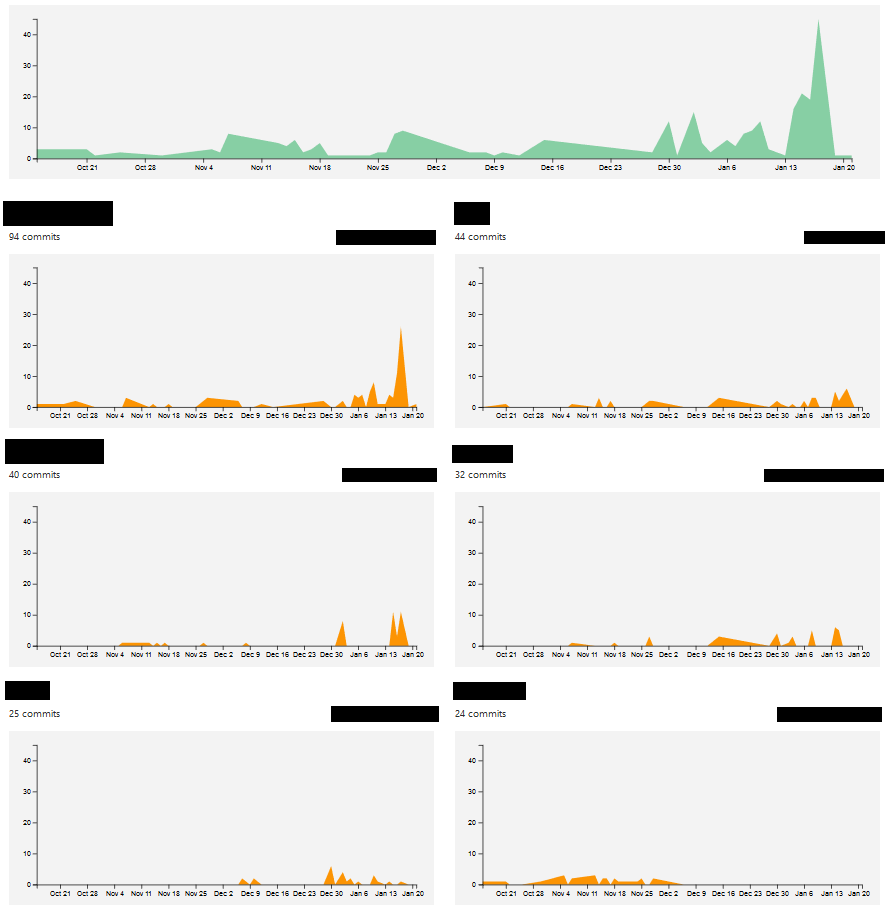
\includegraphics[scale=0.4]{slike/aktivnost.PNG} %veličina slike u odnosu na originalnu datoteku i pozicija slike
			\centering
			\caption{Primjer slike s potpisom}
			\label{fig:promjene}
		\end{figure}
		
		\begin{figure}[H]
			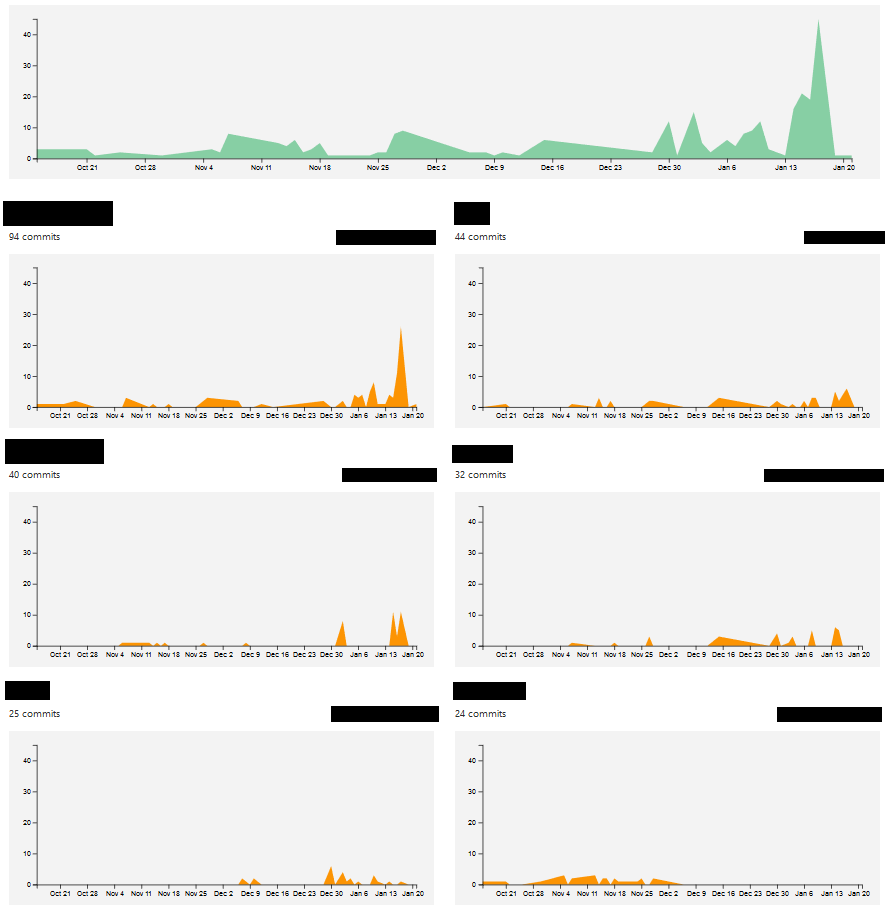
\includegraphics[width=\textwidth]{slike/aktivnost.PNG} %veličina u odnosu na širinu linije
			\caption{Primjer slike s potpisom 2}
			\label{fig:promjene2} %label mora biti drugaciji za svaku sliku
		\end{figure}
		
		Referenciranje slike \ref{fig:promjene2} u tekstu.
		
\end{comment}
		\eject
		
	
	\chapter{Specifikacija programske potpore}
		
	\section{Funkcionalni zahtjevi}
			
	%		\textbf{\textit{dio 1. revizije}}\\
		    
		%	\par{Navesti \textbf{dionike} koji imaju \textbf{interes u ovom sustavu} ili  \textbf{su nositelji odgovornosti}. To su prije svega korisnici, ali i administratori sustava, naručitelji, razvojni tim.}\\
				
	%		\textit{Navesti \textbf{aktore} koji izravno \textbf{koriste} ili \textbf{komuniciraju sa sustavom}. Oni mogu imati inicijatorsku ulogu, tj. započinju određene procese u sustavu ili samo sudioničku ulogu, tj. obavljaju određeni posao. Za svakog aktora navesti funkcionalne zahtjeve koji se na njega odnose.}\\
			
			
			\noindent \textbf{Dionici:}
			
			\begin{packed_enum}
				
				\item Naručitelj projekta (zavod za javno zdravstvo, Crveni križ...)
				\item Razvojni tim
				\item Donori
				\item Djelatnici banke krvi
				\item Administratori sustava
				\item Svi korisnici interneta koji koriste javnu stranicu sustava radi pregleda trenutne razine krvi
				
			\end{packed_enum}
			
			\noindent \textbf{Aktori i njihovi funkcionalni zahtjevi:}
			
			
			\begin{packed_enum}
				\item  \underbar{Administrator (inicijator) može:}
				
				\begin{packed_enum}
					
					\item Administrirati korisničke račune:
					\begin{packed_enum}
						
						\item  Dodati račun djelatnika banke
				    	\item Deaktivirati bilo koji račun u sustavu
				    	\item Definirati optimalne granice razina krvi
				
					\end{packed_enum}
					
				\end{packed_enum}
			
				\item  \underbar{Djelatnik banke (inicijator) može:}
				
				\begin{packed_enum}
					
					\item Prikupiti podatke o donoru
					\begin{packed_enum}
						
						\item Prikupiti matične i kontakt podatke
						\item Prikupiti zdravstvene podatke (krvna grupa)
				
					\end{packed_enum}
					\item Stvoriti korisnički račun donora
					\item Nadopuniti podatke postojećeg računa donora (ukljućujući i zdravstvene podatke)
					\item Evidentirati pokušaj doniranja
					\begin{packed_enum}
						
						\item Zabilježiti trenutne zdravstvene podatke o donoru
						\item  Zabilježiti uspješnost pokušaja doniranja
				
					\end{packed_enum}
					\item Evidentirati trajno odbijanje donora (postojanje + razlog)
					\item Povećati zalihu krvi u sustavu uspješnim doniranjem
					\item Evidentirati slanje krvi u vanjsku instituciju (bolnicu)
					
				\end{packed_enum}
				
				\item  \underbar{Djelatnik banke (sudionik) može:}
				
				\begin{packed_enum}
					
					\item Primiti obavijest o prekoračenju bilo koje od optimalnih granica zaliha krvi
					\item Primiti aktivacijski link radi aktivacije računa
					
				\end{packed_enum}
				
				\item  \underbar{Donor (inicijator) može:}
				
				\begin{packed_enum}
					
					\item Krearati svoj korisnički račun prije prvog darivanja
					\item Nadopuniti podatke računa (osim zdravstvenih podataka - krvne grupe i trajnog odbijanja)
					\item Pregledati povijest darivanja krvi
					\item Preuzeti PDF potvrdu o postojećem doniranju krvi
					
				\end{packed_enum}
				
				
				\item  \underbar{Donor (sudionik) može:}
				
				\begin{packed_enum}
					
					\item Primiti aktivacijski link radi aktivacije računa
					\item Dobiti generirani donorID
					\item Primiti upozorenje o prekoračenju donje optimalne granice zaliha krvi (ako donor nije trajno odbijen)
					\item Pri spajanju u sustav dobiti informaciju o trenutnim zalihama krvi svoje krvne grupe (ako donor nije trajno odbijen)
					\item Primiti obavijest o isteku perioda zabrane darivanja u trajanju od 3 do 4 mjeseca od zadnjeg darivanja
					\item Primiti e-mail s PDF potvrdom o darivanju (nakon darivanja i nakon vlastitog iniciranja izdavanja potvrde)
					
				\end{packed_enum}
				
				\item  \underbar{Korisnik javnog weba (inicijator) može:}
				
				\begin{packed_enum}
					
					\item Krearati novi korisnički račun donora
					\item Pregledati trenutno stanje zaliha krvi svake krvne grupe
					
				\end{packed_enum}
				
				\item  \underbar{Baza podataka (inicijator) može:}
				
				\begin{packed_enum}
					
					\item Izdati obavijest o isteku nedopuštenog perioda darivanja u trajanju od tri do četiri mjeseca
					
				\end{packed_enum}
				
				\item  \underbar{Baza podataka (sudionik) može:}
				
				\begin{packed_enum}
					
					\item Pohranjivati:
					
					    \begin{itemize}
					        \item Postojeće račune u sustavu
					        \item Podatke o donorima
					        \item Podatke o djelatnicima banke
					        \item Količine doza krvi svake krvne grupe u sustavu
					        \item Pokušaje doniranja i sve podatke vezane uz njih
					        \item Potrošnju krvi u sustavu
					    \end{itemize}
					
				\end{packed_enum}
				
			\end{packed_enum}
			
			\eject 
			
			
				
			\subsection{Obrasci uporabe}
				
				%\textbf{\textit{dio 1. revizije}}
				
				\subsubsection{Opis obrazaca uporabe}
				%	\textit{Funkcionalne zahtjeve razraditi u obliku obrazaca uporabe. Svaki obrazac je potrebno razraditi prema donjem predlošku. Ukoliko u nekom koraku može doći do odstupanja, potrebno je to odstupanje opisati i po mogućnosti ponuditi rješenje kojim bi se tijek obrasca vratio na osnovni tijek.}\\
					
                \par {
                    *Baza podataka sudionik je u svim obrascima uporabe, stoga ju ne navodimo zasebno u svakom obrascu (ako je u nekom obrascu posebno navedena, to je kako bi se naglasilo da je u tom obrascu baza podataka glavni sudionik)
                } \\ \\
					\noindent \underbar{\textbf{UC1.1 - Stvori novi račun donora}} \label{UC1.1}
					\begin{packed_item}
	
						\item \textbf{Glavni sudionik: }djelatnik banke
						\item  \textbf{Cilj:} Stvaranje novog računa donora u sustavu pri doniranju krvi
						\item  \textbf{Sudionici:} donor
						\item  \textbf{Preduvjet:} Donor nema stvoren račun, djelatnik banke je prijavljen u sustav (\hyperref[UC3.1]{UC3.1})
						\item  \textbf{Opis osnovnog tijeka:}
						
						\item[] \begin{packed_enum}
							\item Djelatnik banke otvara obrazac za stvaranje pokušaja doniranja
							\item Djelatnik banke otvara obrazac za stvaranje računa donora
							\item Djelatnik banke unosi potrebne podatke o donoru koje saznaje ispitivanjem (matični i kontakt podatci, krvna grupa)
							\item Djelatnik banke pokreće stvaranje računa klikom na gumb \textit{Kreiraj račun}
							\item Sustav validira podatke
							\item Sustav stvara račun u bazi podataka, baza podataka generira donorID
							\item Djelatniku banke na ekran se ispisuje poruka o uspješno izrađenom računu
							\item Pokreće se \hyperref[UC2]{UC2} (\textit{Pošalji e-mail za aktivaciju} - novom donoru)
						\end{packed_enum}
						
						\item  \textbf{Opis mogućih odstupanja:}
						
						\item[] \begin{packed_item}
	
							\item[2.a] Donor nema / ne zna neki od obveznih podataka
							\begin{packed_enum}
								\item Proces se neuspješno završava
							\end{packed_enum}
							
							\item[2.b] Donor ne zna svoju krvnu grupu
                            \begin{packed_enum}
							    \item Djelatnik banke testom određuje krvnu grupa donora
							    \item Djelatnik banke upisuje krvnu grupu u račun donora
							    \item Proces kreiranja računa nastavlja se gdje je i stao na koraku 2 osnovnog tijeka
                            \end{packed_enum}
						
							\item[4.a] Dani podatci su sintaksno pogrešni
							\begin{packed_enum}
								\item Sustav na ekran ispisuje poruku o neispravnosti unesenih podataka
								\item Proces se nastavlja na koraku 2 osnovnog tijeka
							\end{packed_enum}
							
							\item[4.b] Unesen je podatak koji je već evidentiran kod nekog drugog donora, a radi se o podatku koji mora biti jedinstven
							\begin{packed_enum}
								\item Sustav na ekran ispisuje poruku o nejedinstvenosti unesenog podatka
								\item Proces se nastavlja na koraku 2 osnovnog tijeka
							\end{packed_enum}
							
						\end{packed_item}
						
					\end{packed_item}
					
					\noindent \underbar{\textbf{UC1.2 - Stvori novi račun sebi}}
					\begin{packed_item}
	
						\item \textbf{Glavni sudionik: }donor
						\item  \textbf{Cilj:} Osobno stvaranje novog računa donora u sustavu
						\item  \textbf{Sudionici:} 
						\item  \textbf{Preduvjet:} Donor nema stvoren račun, donor ima pristup internetu
						\item  \textbf{Opis osnovnog tijeka:}
						
						\item[] \begin{packed_enum}
                        	\item Donor otvara obrazac za registraciju
							\item Donor unosi potrebne podatke (matični i kontakt podatci, ne i krvna grupa)
							\item Donor pokreće stvaranje računa klikom na gumb \textit{Kreiraj račun}
							\item Sustav validira podatke 
							\item Sustav stvara račun u bazi podataka, baza podataka generira donorID
							\item Donoru se na ekran ispisuje poruka o uspješno izrađenom računu
							\item Pokreće se \hyperref[UC2]{UC2} (\textit{Pošalji e-mail za aktivaciju} - novom donoru)
						\end{packed_enum}
						
						\item  \textbf{Opis mogućih odstupanja:}
						
						\item[] \begin{packed_item}
	
                        	\item[2.a] Donor nema / ne zna neki od obveznih podataka
							\begin{packed_enum}
								\item Proces se neuspješno završava
							\end{packed_enum}
						
							\item[4.a] Dani podatci su sintaksno pogrešni
							\begin{packed_enum}
								\item Sustav na ekran ispisuje poruku o neispravnosti unesenih podataka
								\item Proces se nastavlja na koraku 2 osnovnog tijeka
							\end{packed_enum}
							
							\item[4.b] Unesen je podatak koji je već evidentiran kod nekog drugog donora, a radi se o podatku koji mora biti jedinstven
							\begin{packed_enum}
								\item Sustav na ekran ispisuje poruku o nejedinstvenosti unesenog podatka
								\item Proces se nastavlja na koraku 2 osnovnog tijeka
							\end{packed_enum}
							
						\end{packed_item}
						
					\end{packed_item}
					
					\noindent \underbar{\textbf{UC1.3 - Stvori novi račun djelatnika banke}}
					\begin{packed_item}
	
						\item \textbf{Glavni sudionik: }administrator
						\item  \textbf{Cilj:} Stvaranje novog računa djelatnika banke u sustavu
						\item  \textbf{Sudionici:} djelatnik banke
						\item  \textbf{Preduvjet:} Djelatnik banke nema stvoren račun, administrator ima sve potrebne podatke, administrator je prijavljen u sustav (\hyperref[UC3.1]{UC3.1})
						\item  \textbf{Opis osnovnog tijeka:}
						
						\item[] \begin{packed_enum}
                        	\item Administrator otvara obrazac za stvaranje računa djelatnika banke
							\item Administrator unosi potrebne podatke (matične i kontakt podatke djelatnika banke)
							\item Administrator pokreće stvaranje računa klikom na gumb \textit{Kreiraj račun}
							\item Sustav validira podatke 
							\item Sustav stvara račun u bazi podataka, baza podataka generira bankworkerID
							\item Administratoru se na ekran ispisuje poruka o uspješno izrađenom računu djelatnika
							\item Pokreće se \hyperref[UC2]{UC2} (\textit{Pošalji e-mail za aktivaciju} - novom djelatniku banke)
						\end{packed_enum}
						
						\item  \textbf{Opis mogućih odstupanja:}
						
						\item[] \begin{packed_item}
	
                        	\item[2.a] Administrator nema / ne zna neki od obveznih podataka
							\begin{packed_enum}
								\item Proces se neuspješno završava
							\end{packed_enum}
						
							\item[4.a] Dani podatci su sintaksno pogrešni
							\begin{packed_enum}
								\item Sustav na ekran ispisuje poruku o neispravnosti unesenih podataka
								\item Proces se nastavlja na koraku 2 osnovnog tijeka
							\end{packed_enum}
							
							
							\item[4.b] Unesen je podatak koji je već evidentiran kod nekog drugog djelatnika banke, a radi se o podatku koji mora biti jedinstven
							\begin{packed_enum}
								\item Sustav na ekran ispisuje poruku o nejedinstvenosti unesenog podatka
								\item Proces se nastavlja na koraku 2 osnovnog tijeka
							\end{packed_enum}
							
						\end{packed_item}
						
					\end{packed_item}
					
					%\noindent \underbar{\textbf{UC1.4 - Stvori novi račun administratora}}
					%\begin{packed_item}
	
					%	\item \textbf{Glavni sudionik: }administrator
					%	\item  \textbf{Cilj:} Stvaranje novog računa administratora u sustavu
					%	\item  \textbf{Sudionici:} 
					%	\item  \textbf{Preduvjet:} Postoji bar jedan administrator u sustavu, administrator je prijavljen u sustav (\hyperref[UC3.1]{UC3.1})
					%	\item  \textbf{Opis osnovnog tijeka:}
						
					%	\item[] \begin{packed_enum}
                    %    	\item Administrator otvara obrazac za stvaranje računa administratora
					%		\item Administrator unosi e-adresu novog administratora (koja se ne sprema trajno)
					%		\item Administrator pokreće stvaranje računa klikom na gumb \textit{Kreiraj račun}
					%		\item Sustav validira e-adresu 
					%		\item Sustav stvara račun u bazi podataka (generira lozinku), baza podataka generira userID
					%		\item Administratoru se na ekran ispisuje generirani userID
					%		\item Pokreće se \hyperref[UC2]{UC2} (Pošalji e-mail za aktivaciju - novom administratoru)
					%	\end{packed_enum}

					%	\item  \textbf{Opis mogućih odstupanja:}
						
					%	\item[] \begin{packed_item}
	
					%		\item[4] E-adresa je sintaksno pogrešna
					%		\begin{packed_enum}
					%			\item Sustav na ekran ispisuje poruku o neispravnosti e-adrese
					%			\item Proces se nastavlja na koraku 2 osnovnog tijeka
					%		\end{packed_enum}
							
					%	\end{packed_item}
						
					%\end{packed_item}
					
					\noindent \underbar{\textbf{UC2 - Pošalji e-mail za aktivaciju}}
					\begin{packed_item} \label{UC2}
	
						\item \textbf{Glavni sudionik: } korisnik sustava (donor, djelatnik banke ili administrator)
						\item  \textbf{Cilj:} Poslati e-mail s korisničkim podatcima i poveznicom za aktivaciju računa
						\item  \textbf{Sudionici:} 
						\item  \textbf{Preduvjet:} Novi korisnik pokrenuo je stvaranje računa; sustav ima generirane userID i inicijalnu lozinku
						\item  \textbf{Opis osnovnog tijeka:}
						
						\item[] \begin{packed_enum}
	                        \item Sustav generira poveznicu za aktivaciju računa
	                        \item Sustav generira e-poruku s navedenom poveznicom za aktivaciju te inicijalnim podatcima za prijavu
	                        \item Sustav na e-adresu definiranu pri kreiranju računa šalje e-poruku s generiranim podatcima
						\end{packed_enum}
						
						\item  \textbf{Opis mogućih odstupanja:}
						
					\end{packed_item}
					
					
					\noindent \underbar{\textbf{UC3 - Aktiviraj svoj račun}}
					\begin{packed_item}  \label{UC3}
	
						\item \textbf{Glavni sudionik: }novi korisnik sustava (donor, djelatnik banke ili administrator)
						\item  \textbf{Cilj:} Aktivirati korisnički račun radi buduće prijave u sustav
						\item  \textbf{Sudionici:} 
						\item  \textbf{Preduvjet:} Novi korisnik sustava ima generiran račun, korisnički podatci dostavljeni su na e-adresu, korisnik sustava ima pristup korisničkim podatcima
						\item  \textbf{Opis osnovnog tijeka:}
						
						\item[] \begin{packed_enum}
	
	                        \item Korisnik pristupa poveznici za aktivaciju računa
	                        \item Sustav u bazi podataka evidentira račun kao aktiviran

						\end{packed_enum}
						
						\item  \textbf{Opis mogućih odstupanja:}
						
					\end{packed_item}
					
					\noindent \underbar{\textbf{UC3.1 - Prijavi se u sustav}}
					\begin{packed_item}  \label{UC3.1}
	
						\item \textbf{Glavni sudionik: }korisnik sustava
						\item  \textbf{Cilj:} Prijaviti se u sustav i dobiti pristup značajkama dostupnima samo prijavljenim korisnicima
						\item  \textbf{Sudionici:} 
						\item  \textbf{Preduvjet:} Korisnik sustava ima generiran račun, korisnik sustava ima pristup korisničkim podatcima
						\item  \textbf{Opis osnovnog tijeka:}
						
						\item[] \begin{packed_enum}
	                        \item Korisnik na početnoj stranici pritišće gumb \textit{Prijavi se}
	                        \item Korisnik u polja za prijavu unosi svoj userID (donorID, bankworkerID) i lozinku
	                        \item Korisnik pritiskom na gumb \textit{Prijava} pokreće proces prijave u sustav
	                        \item Sustav provjerava ispravnost podataka i nakon potvrde vraća kolačić s identifikatorom sjednice
	                        \item Sustav preusmjerava korisnika na početnu stranicu profila
						\end{packed_enum}
						
						\item  \textbf{Opis mogućih odstupanja:}
						\item[] \begin{packed_enum}
						
	                        \item[4.a] Korisnik nema aktiviran račun
	                        \item[] \begin{packed_enum}
    	                        \item Sustav na ekran ispisuje poruku o nemogućnosti prijave zbog neaktiviranog računa
    	                        \item Proces se prekida
					    	\end{packed_enum}
					    	
	                        \item[4.b] Korisnik je unio neki od pogrešnih podataka za prijavu
	                        \item[] \begin{packed_enum}
    	                        \item Sustav na ekran ispisuje poruku o nemogućnosti prijave zbog neispravnih podataka za prijavu
    	                        \item Proces se nastavlja na koraku 2 osnovnog tijeka
					    	\end{packed_enum}
						\end{packed_enum}
						
					\end{packed_item}
					
						
					\noindent \underbar{\textbf{UC4 - Pregledaj svoje podatke}}
					\begin{packed_item}  \label{UC4}
	
						\item \textbf{Glavni sudionik: }donor
						\item  \textbf{Cilj:} Pregledati podatke računa trenutnog korisnika
						\item  \textbf{Sudionici:} djelatnik banke
						\item  \textbf{Preduvjet:} Trenutni korisnik ima račun i prijavljen je u sustav (\hyperref[UC3.1]{UC3.1})
						\item  \textbf{Opis osnovnog tijeka:}
						
						\item[] \begin{packed_enum}
	
	                        \item Korisnik na podstranici \textit{Profil} pritišće gumb \textit{Uredi podatke}
	                        \item Sustav učitava stranicu s postojećim podatcima i gumbom za uređivanje podataka

						\end{packed_enum}
						
						\item  \textbf{Opis mogućih odstupanja:}

						
					\end{packed_item}
					
					
					\noindent \underbar{\textbf{UC4.1 - Pronađi i pregledaj podatke donora}}
					\begin{packed_item}  \label{UC4.1}
	
						\item \textbf{Glavni sudionik: }djelatnik banke
						\item  \textbf{Cilj:} Pronaći donora u sustavu i pregledati njegove podatke
						\item  \textbf{Sudionici:} administrator
						\item  \textbf{Preduvjet:} Donor ima generiran račun, trenutni korisnik je prijavljen u sustav (\hyperref[UC3.1]{UC3.1}) i ima dovoljno podataka o donoru kako bi ga pronašao u sustavu
						\item  \textbf{Opis osnovnog tijeka:}
						\\ *Korisnikom se smatra djelatnik banke ili administrator
						\item[] \begin{packed_enum}
	                    
	                        \item Korisnik pristupa obrascu za traženje donora klikom na gumb \textit{Pronađi donora} na stranici za stvaranje pokušaja doniranja ili na stranici za deaktivaciju računa
	                        \item Korisnik u obrazac unosi neki od podataka donora (donorID, OIB, ime, prezime) ili više njih u kombinaciji, odvojene razmakom
	                        \item Sustav iz baze podataka dobavlja podatke o traženim donorima
	                        \item Sustav u tabličnom prikazu ispisuje sve donore kojima se osobni podatci podudaraju s traženima
	                        \item Korisnik odabire željenog donora klikom na željeni redak
	                        \item Sustav preusmjerava korisnika na prethodnu stranicu s koje je došao, pritom noseći i podatak o odabranom donoru

						\end{packed_enum}
						
						\item  \textbf{Opis mogućih odstupanja:}
						\item[] \begin{packed_item}
	
							\item[3.1] Sustav od baze podataka ne dobiva podatke jer ne postoji donor s navedenim podatcima
							\item[] \begin{packed_enum}
								\item Sustav na ekran ispisuje da nema pronađenih rezultata
								\item Izvođenje se nastavlja na koraku 2 osnovnog tijeka
							\end{packed_enum}
							\item[3.2] Traženi račun je trajno deaktiviran
							\item[] \begin{packed_enum}
								\item Sustav iz baze podataka dobavlja podatke samo o nedeaktiviranim korisnicima
								\item Baza podataka ne pronalazi zapis traženog donora
								\item Sustav na ekran ispisuje da nema pronađenih rezultata
								\item Izvođenje se nastavlja na koraku 2 osnovnog tijeka
							\end{packed_enum}
							
						\end{packed_item}
						
					\end{packed_item}
					
					
					\noindent \underbar{\textbf{UC4.2 - Pronađi i pregledaj podatke djelatnika banke}}
					\begin{packed_item}  \label{UC4.2}
	
						\item \textbf{Glavni sudionik: }administrator
						\item  \textbf{Cilj:} Pronaći djelatnika banke u sustavu i pregledati njegove podatke
						\item  \textbf{Sudionici:} 
						\item  \textbf{Preduvjet:} Djelatnik banke ima generiran račun, administrator je prijavljen u sustav (\hyperref[UC3.1]{UC3.1}), administrator ima dovoljno podataka o djelatniku banke kako bi ga pronašao u sustavu
						\item  \textbf{Opis osnovnog tijeka:}
						
						\item[] \begin{packed_enum}
	                        \item Administrator pristupa obrascu za traženje djelatnika banke klikom na gumb \textit{Pronađi djelatnika} sa stranice za deaktivaciju računa
	                        \item Administrator u obrazac unosi neki od podataka donora (donorID, OIB, ime, prezime) ili više njih u kombinaciji, odvojene razmakom
	                        \item Sustav iz baze podataka dobavlja podatke o traženim djelatnicima banke
	                        \item Sustav u tabličnom prikazu ispisuje sve djelatnike banke kojima se osobni podatci podudaraju s traženima
	                        \item Administrator odabire željenog djelatnika banke klikom na željeni redak
	                        \item Sustav preusmjerava administratora na prethodnu stranicu s koje je došao, pritom noseći i podatak o odabranom djelatniku banke
						\end{packed_enum}
						
						\item  \textbf{Opis mogućih odstupanja:}
						\item[] \begin{packed_item}
	
							\item[3.1] Sustav od baze podataka ne dobiva podatke jer ne postoji djelatnik banke s navedenim podatcima
							\item[] \begin{packed_enum}
								\item Sustav na ekran ispisuje poruku o neuspješnom dohvaćanju djelatnika banke
								\item Izvođenje se nastavlja na koraku 2 osnovnog tijeka
							\end{packed_enum}
							\item[3.2] Traženi račun je trajno deaktiviran
							\item[] \begin{packed_enum}
								\item Sustav iz baze podataka dobavlja podatke samo o nedeaktiviranim korisnicima
								\item Baza podataka ne pronalazi zapis traženog djelatnika banke
								\item Sustav na ekran ispisuje da nema pronađenih rezultata
								\item Izvođenje se nastavlja na koraku 2 osnovnog tijeka
							\end{packed_enum}
							
						\end{packed_item}
						
					\end{packed_item}
					
					
					\noindent \underbar{\textbf{UC5 - Uredi matične i kontakt podatke donora}}
					\begin{packed_item} \label{UC5}
	
						\item \textbf{Glavni sudionik: }donor
						\item  \textbf{Cilj:} Uređivanje svojih postojećih matičnih i kontakt podataka
						\item  \textbf{Sudionici:} 
						\item  \textbf{Preduvjet: }Donor ima stvoren račun i nalazi se na stranici za uređivanje osobnih podataka (vidi \hyperref[UC4]{UC4 (\textit{Pregledaj svoje podatke})}
						\item  \textbf{Opis osnovnog tijeka:}
						
						\item[] \begin{packed_enum}
	                        \item Donor izmjenjuje potrebne matične ili kontakt podatake (ali ne i zdravstvene podatke)
	                        \item Donor pritišće gumb \textit{Pohrani promjene}
	                        \item Sustav validira ispravnost podataka
	                        \item Sustav ažurira postojeći zapis u bazi podataka
	                        
						\end{packed_enum}
						
						\item  \textbf{Opis mogućih odstupanja:}
						
						\item[] \begin{packed_item}
	
							\item[4.a] Donor želi promijeniti OIB na vrijednost koja više ne bi bila jedinstvena
							\begin{packed_enum}
								\item Sustav ispisuje poruku o nejedinstvenosti podatka te odbija spremiti promjene
								\item Proces se nastavlja na koraku 2 osnovnog tijeka
							\end{packed_enum}
							
							\item[4.b] Dani podatci su sintaksno pogrešni
							\begin{packed_enum}
								\item Sustav na ekran ispisuje poruku o neispravnosti unesenih podataka
								\item Proces se nastavlja na koraku 2 osnovnog tijeka
							\end{packed_enum}
							
						\end{packed_item}
						
					\end{packed_item}
					
					\noindent \underbar{\textbf{UC5.1 - Uredi zdravstvene, matične i kontakt podatke donora}}
					\begin{packed_item} \label{UC5.1}
	
						\item \textbf{Glavni sudionik: }djelatnik banke
						\item  \textbf{Cilj:} Uređivanje postojećih podataka o računu donora
						\item  \textbf{Sudionici:} donor
						\item  \textbf{Preduvjet:} Donor ima stvoren račun, djelatnik banke ga je pronašao koristeći \hyperref[UC4.1]{UC4.1 (\textit{Pronađi i pregledaj podatke donora})} 
						\item  \textbf{Opis osnovnog tijeka:}
						
						\item[] \begin{packed_enum}
	                        \item Djelatnik banke sa stranice za stvaranje pokušaja donacije pristupa obrascu za izmjenu podataka donora klikom na gumb \textit{Uredi podatke}
	                        \item Djelatnik banke izmjenjuje bilo koji potrebni podatak o donoru  (uključujući i zdravstvene podatke)
	                        \item Djelatnik banke pritišće gumb \textit{Pohrani promjene}
	                        \item Sustav validira ispravnost podataka
	                        \item Sustav ažurira postojeći zapis u bazi podataka
	                      %  \item U slučaju neaktualnih podataka, djelatnik banke ažurira podatke
	                      % \item U slučaju da je donor sam stvorio račun, provjerava se krvna grupa donora i djelatnik banke ju unosi u sustav
	                      %  \item Ukoliko se pri evidenciji zdravstvenih podataka u pokušaju doniranja pokaže okolnost za trajno odbijanje donora, pokreće se \hyperref[UC4.3]{UC4.3} (\textit{Evidentiraj trajno odbijanje donora})
						\end{packed_enum}
						
						\item  \textbf{Opis mogućih odstupanja:}
						
						\item[] \begin{packed_item}
	
							\item[4.a] Djelatnik banke želi promijeniti OIB donora na vrijednost koja više ne bi bila jedinstvena
							\begin{packed_enum}
								\item Sustav ispisuje poruku o nejedinstvenosti podatka te odbija spremiti promjene
								\item Proces se nastavlja na koraku 2 osnovnog tijeka
							\end{packed_enum}
							
							\item[4.b] Dani podatci su sintaksno pogrešni
							\begin{packed_enum}
								\item Sustav na ekran ispisuje poruku o neispravnosti unesenih podataka
								\item Proces se nastavlja na koraku 2 osnovnog tijeka
							\end{packed_enum}
							
						\end{packed_item}
						
					\end{packed_item}
					
				
					\noindent \underbar{\textbf{UC5.2 - Uredi podatke djelatnika banke}}
					\begin{packed_item}
	
						\item \textbf{Glavni sudionik: }djelatnik banke
						\item  \textbf{Cilj:} Uređivanje već postojećih podataka 
						\item  \textbf{Sudionici:} 
						\item  \textbf{Preduvjet: }Djelatnik banke ima stvoren račun i nalazi se na stranici za uređivanje osobnih podataka (vidi \hyperref[UC4]{UC4 (\textit{Pregledaj svoje podatke})}
						\item  \textbf{Opis osnovnog tijeka:}
						
						\item[] \begin{packed_enum}
	                        \item Djelatnik banke izmjenjuje potrebni podatak 
	                        \item Djelatnik banke pritišće gumb \textit{Pohrani promjene}
	                        \item Sustav validira ispravnost podataka
	                        \item Sustav ažurira postojeći zapis u bazi podataka
	                        
						\end{packed_enum}
						
						\item  \textbf{Opis mogućih odstupanja:}
						
						\item[] \begin{packed_item}
	
							\item[4.a] Djelatnik banke želi promijeniti OIB na vrijednost koja više ne bi bila jedinstvena
							\begin{packed_enum}
								\item Sustav ispisuje poruku o nejedinstvenosti podatka te odbija spremiti promjene
								\item Proces se nastavlja na koraku 2 osnovnog tijeka
							\end{packed_enum}
							
							\item[4.b] Dani podatci su sintaksno pogrešni
							\begin{packed_enum}
								\item Sustav na ekran ispisuje poruku o neispravnosti unesenih podataka
								\item Proces se nastavlja na koraku 2 osnovnog tijeka
							\end{packed_enum}
							
						\end{packed_item}
						
					\end{packed_item}
					
					
					\noindent \underbar{\textbf{UC5.3 - Deaktiviraj račun}}
					\begin{packed_item} \label{5.3}
	
						\item \textbf{Glavni sudionik: }administrator
						\item  \textbf{Cilj:} Deaktivacija postojećeg računa 
						\item  \textbf{Sudionici:} 
						\item  \textbf{Preduvjet:} Korisnički račun koji se treba deaktivirati postoji
						\item  \textbf{Opis osnovnog tijeka:}
						
						\item[] \begin{packed_enum}
	
	                        \item Administrator pristupa stranici za deaktivaciju računa pritiskom na gumb \textit{Upravljaj računima}
	                        \item Administrator koristi tražilicu kako bi pronašao traženi račun pritiskom na gumb \textit{Pronađi donora} ili \textit{Pronađi djelatnika} (vidi \hyperref[UC4.1]{UC4.1 (\textit{Pronađi i pregledaj podatke donora})} ili \hyperref[UC4.2]{UC4.2 (\textit{Pronađi i pregledaj podatke djelatnika banke})})
							\item Administrator nakon pronalaska računa i povratka na stranicu za deaktivaciju pritišće gumb \textit{Deaktiviraj račun}
	                        \item Sustav u bazi podataka evidentira da je račun deaktiviran (ali račun se ne briše)

						\end{packed_enum}
						
						\item  \textbf{Opis mogućih odstupanja:}
						
					\end{packed_item}
					
					
					\noindent \underbar{\textbf{UC6 - Stvori pokušaj doniranja}}
					\begin{packed_item} \label{UC6}
	
						\item \textbf{Glavni sudionik: }djelatnik banke
						\item  \textbf{Cilj:} Stvaranje pokušaja doniranja, evidentiranje trenutnih zdravstvenih podataka
						\item  \textbf{Sudionici:} donor
						\item  \textbf{Preduvjet:} Donor je došao na doniranje i ima izrađen korisnički račun 
						\item  \textbf{Opis osnovnog tijeka:}
						
						\item[] \begin{packed_enum}
	
							\item Djelatnik banke otvara obrazac za unos novog pokušaja darivanja
							\item Djelatnik banke pronalazi donora u sustavu koristeći tražilicu pritiskom na gumb \textit{Pronađi donora} - vidi \hyperref[UC4.1]{UC4.1 (\textit{Pronađi i pregledaj podatke donora})}
							\item Djelatnik banke u sustavu ispunjava zdravstveni upitnik prema odgovorima koje mu daje donor
	                        \item Djelatnik banke pritiskom na gumb \textit{Spremi pokušaj doniranja} pokreće proces spremanja
	                        \item Donor odlazi darivati krv, a pokušaj doniranja evidentira se kao uspješan
	                        \item Sustav u bazi podataka stvara novi pokušaj doniranja s prethodno navedenim podatcima
	                        \item Sustav u bazi podataka evidentira povećanje zalihe krvi krvne grupe donora iz ovog pokušaja za jednu dozu
	                        \item Sustav generira PDF potvrdu o darivanju krvi
	                        \item Djelatniku banke na ekran se ispisuje poruka o uspješnom darivanju krvi
	                        \item Sustav šalje potvrdu na mail (vidi \hyperref[UC12]{UC12} za sličnu funkcionalnost gdje se potvrda preuzima na računalo)

						\end{packed_enum}
						
						\item  \textbf{Opis mogućih odstupanja:}
						
						\item[] \begin{packed_item}
	
							\item[4.a] Neki od zdravstvenih podataka implicira privremeno odbijanje donora
							\begin{packed_enum}
								\item Sustav pokušaj doniranja evidentira kao neuspješan
								\item Obavlja se korak 6 osnovnog tijeka (spremanje pokušaja doniranja)
								\item Djelatniku banke se na ekran ispisuje poruka o neuspješnom darivanju krvi
								\item Proces završava
							\end{packed_enum}
							
							\item[4.b] Neki od zdravstvenih podataka implicira trajno odbijanje donora
							\begin{packed_enum}
								\item Sustav pokušaj doniranja evidentira kao neuspješan
								\item Sustav evidentira trajno odbijanje u računu donora s razlogom odbijanja poslanom u obrascu
								\item Obavlja se korak 6 osnovnog tijeka (spremanje pokušaja doniranja)
								\item Djelatniku banke se na ekran ispisuje poruka o neuspješnom darivanju krvi
								\item Proces završava
							\end{packed_enum}
							
							\item[7] S novom dozom krvi prekoračuje se gornja optimalna granica zaliha doza krvi
							\begin{packed_enum}
							    \item Pokreće se \hyperref[UC14]{UC14 (\textit{Izdaj upozorenje o prekoračenju optimalne granice})}
								\item Proces se nastavlja gdje je i stao na koraku 7 osnovnog tijeka
							\end{packed_enum}
							
						\end{packed_item}
						
					\end{packed_item}
					
					
					\noindent \underbar{\textbf{UC7 - Pregledaj zalihe svih krvnih grupa}}
					\begin{packed_item}
	
						\item \textbf{Glavni sudionik: }korisnik interneta
						\item  \textbf{Cilj:} Na javnom webu pregledati stanja svih krvnih grupa i dobiti informaciju o stanju zaliha svake grupe u odnosu na optimalne granice
						\item  \textbf{Sudionici:}
						\item  \textbf{Preduvjet:} 
						\item  \textbf{Opis osnovnog tijeka:}
						
						\item[] \begin{packed_enum}
	
	                        \item Korisnik interneta pristupa početnoj stranici aplikacije
	                        \item Sustav dohvaća trenutna stanja zaliha krvi i optimalne granice za svaku krvnu grupu iz baze podataka
	                        \item Sustav vizualno prikazuje stanja zaliha svih krvnih grupa i njihovih optimalnih granica tako da je gornja optimalna granica na 90\% visine, donja optimalna granica i trenutna razina krvi proporcionalno tome (donja optimalna granica na visini od donjaGranica/gornjaGranica*90\%, a trenutna razina krvi na visini od razina/gornjaGranica*90\%)
	                        \item Sustav provjerava nalaze li se sva stanja zaliha između optimalnih granica

						\end{packed_enum}
						
						\item  \textbf{Opis mogućih odstupanja:}
						
						\item[] \begin{packed_item}
	
							\item[4] Neko stanje zaliha nalazi se ispod donje optimalne granice za tu krvnu grupu 
							\begin{packed_enum}
								\item Sustav na stranici ispisuje i poruku o nedostatku krvnih grupa čije je stanje ispod donje optimalne granice
								\item Proces završava
							\end{packed_enum}
							
						\end{packed_item}
						
					\end{packed_item}
					
					
					%\noindent \underbar{\textbf{UC8 - Promijeni lozinku}}
					%\begin{packed_item}
	
						%\item \textbf{Glavni sudionik: }prijavljeni korisnik
						%\item  \textbf{Cilj:} Promijeniti lozinku svog računa
						%\item  \textbf{Sudionici:} 
						%\item  \textbf{Preduvjet:} Korisnik ima podatke za prijavu, prijavljen je u sustav (\hyperref[UC3.1]{UC3.1}) i ima potrebu za promjenom lozinke
						%\item  \textbf{Opis osnovnog tijeka:}
						
						%item[] \begin{packed_enum}
	                        %\item Korisnik s profila otvara obrazac za promjenu lozinke pritiskom na gumb \textit{Promijeni lozinku}
	                        %\item Korisnik unosi staru i novu lozinku te pokreće validaciju i promjenu lozinke pritiskom na gumb \textit{Promijeni lozinku}
	                        %\item Sustav validira lozinku
	                        %\item Sustav u bazi podataka evidentira promjenu lozinke
	                        %\item Sustav korisniku na ekran ispisuje poruku o uspješno promijenjenoj lozinki
						%\end{packed_enum}
						
						%\item  \textbf{Opis mogućih odstupanja:}
						
						%\item[] \begin{packed_item}
	
							%\item[3] Lozinka je nesigurna (definirano u ostalim zahtjevima)
							%\begin{packed_enum}
								%\item Sustav na ekran ispisuje prikladnu poruku koja navodi korisnika na pravila za sastavljanje sigurne lozinke
								%\item Proces se nastavlja na koraku 2 osnovnog tijeka
							%\end{packed_enum}
							
						%\end{packed_item}
						
					%\end{packed_item}
					
					
					\noindent \underbar{\textbf{UC9 - Definiraj optimalne granice zaliha krvi}}
					\begin{packed_item} \label{UC9}
	
						\item \textbf{Glavni sudionik: }administrator
						\item  \textbf{Cilj:} Postaviti gornje i donje optimalne granice za svaku krvnu grupu
						\item  \textbf{Sudionici:} 
						\item  \textbf{Preduvjet:} Administrator ima korisnički račun i prijavljen je u sustav (\hyperref[UC3.1]{UC3.1})
						\item  \textbf{Opis osnovnog tijeka:}
						
						\item[] \begin{packed_enum}
							\item Administrator pristupa obrascu za postavljanje optimalnih granica pritiskom na gumb \textit{Uredi granice}
	                        \item Administrator za svaku krvnu grupu podešava gornje i donje optimalne granice zaliha krvi
	                        \item Administrator pokreće proces spremanja pritiskom na gumb \textit{Spremi granice}
	                        \item Sustav sprema promjene u bazu podataka
						\end{packed_enum}
						
						\item  \textbf{Opis mogućih odstupanja:}
						
						\item[] \begin{packed_item}
	
							\item[3] Administrator podešava novu donju optimalnu granicu iznad trenutne zalihe krvi, ili gornju optimalnu granicu ispod trenutne zalihe krvi za bilo koju krvnu grupu
							\item[] \begin{packed_enum}
                                \item Pokreće se \hyperref[UC14]{UC14 (\textit{Izdaj upozorenje o prekoračenju optimalne granice})}
                                \item Proces se nastavlja gdje je i stao na koraku 3 osnovnog tijeka
							\end{packed_enum}

						\end{packed_item}
						
					\end{packed_item}
					
					
					\noindent \underbar{\textbf{UC10 - Ispiši poruku o stanju zalihe krvne grupe donora}}
					\begin{packed_item}
	
						\item \textbf{Glavni sudionik: }donor
						\item  \textbf{Cilj:} Informirati donora o okvirnom stanju zaliha njegove krvne grupe
						\item  \textbf{Sudionici:} 
						\item  \textbf{Preduvjet:} Donor je prijavljen u sustav (\hyperref[UC3.1]{UC3.1}) i nedostaje njegove krvne grupe
						\item  \textbf{Opis osnovnog tijeka:}
						
						\item[] \begin{packed_enum}
	
							\item Donor dolazi na početnu stranicu prijavljenog korisnika (profil)
	                        \item Sustav na ekranu prikazuje poruku o nedostatku zalihe te krvne grupe

						\end{packed_enum}
						
						\item  \textbf{Opis mogućih odstupanja:}
						
						\item[] \begin{packed_item}
	
							\item[2] Stanje zaliha krvi je iznad donje optimalne granice
							\item[] \begin{packed_enum}
								\item Poruka se ne ispisuje
								\item Proces završava
							\end{packed_enum}
							
							\item[2] Stanje zaliha krvi je ispod donje optimalne granice
							\item[] \begin{packed_enum}
								\item Sustav ispisuje dodatno istaknutu poticajnu poruku za darivanje krvi
								\item Proces završava
							\end{packed_enum}

						\end{packed_item}
						
					\end{packed_item}
					
					
					\noindent \underbar{\textbf{UC11 - Pregledaj povijest pokušaja doniranja}}
					\begin{packed_item} \label{UC11}
	
						\item \textbf{Glavni sudionik: }donor
						\item  \textbf{Cilj:} Dati donoru uvid u sve svoje prijašnje pokušaje doniranja i njihov ishod, te ponuditi mogućnsot preuzimanja potvrde
						\item  \textbf{Sudionici:} djelatnik banke
						\item  \textbf{Preduvjet:} Donor je prijavljen u sustav (\hyperref[UC3.1]{UC3.1}) / djelatnik banke je pronašao donora u sustavu pri darivanju
						\item  \textbf{Opis osnovnog tijeka:}
						
						*Korisnikom se smatra donor ili djelatnik banke opisani u preduvjetima
						\item[] \begin{packed_enum}
							\item Korisnik otvara stranicu s povijesti pokušaja doniranja pritiskom na gumb \textit{Moje donacije / Prošle donacije}
	                        \item Sustav za svaki pokušaj doniranja navodi osnovne podatke definirane u ostalim zahtjevima
	                        \item Sustav za svaki uspješni pokušaj stvara i gumb \textit{Preuzmi}
						\end{packed_enum}
						
						\item  \textbf{Opis mogućih odstupanja:}
						
						\item[] \begin{packed_item}
	
							\item[2] Korisnik nema nijedan prethodan pokušaj doniranja
							\item[] \begin{packed_enum}
								\item Sustav ispisuje informativnu poruku o nepostojanju prijašnjih darivanja
								\item Proces završava
							\end{packed_enum}
							
							\item[3] Korisnik pritišće gumb \textit{Preuzmi} za neki pokušaj doniranja
							\item[] \begin{packed_enum}
							    \item Pokreće se (\hyperref[UC12]{UC12 - \textit{Preuzmi PDF potvrdu}}) od koraka 2 osnovnog tijeka
							\end{packed_enum}

						\end{packed_item}
						
					\end{packed_item}
					
					\noindent \underbar{\textbf{UC12 - Preuzmi PDF potvrdu}}
					\begin{packed_item} \label{UC12}
	
						\item \textbf{Glavni sudionik: }donor
						\item  \textbf{Cilj:} Preuzimanje PDF potvrde o pokušaju doniranja iz povijesti doniranja u sustavu
						\item  \textbf{Sudionici:} djelatnik
						\item  \textbf{Preduvjet:} Donor se nalazi na stranici s prethodnim pokušajima doniranja i ima obavljeno barem jedno uspješno doniranje / djelatnik banke pronašao je donora u sustavu i pristupio je stranici s njegovim prijašnjim donacijama (vidi \hyperref[UC11]{UC11})
						\item  \textbf{Opis osnovnog tijeka:}
						
						*Korisnikom se smatra donor ili djelatnik banke opisani u preduvjetima
						\item[] \begin{packed_enum}
	                        \item Korisnik pritišće gumb \textit{Preuzmi PDF potvrdu} 
	                        \item Sustav generira PDF potvrdu o doniranju
	                        \item Sustav pokreće preuzimanje PDF potvrde na računalo korisnika
						\end{packed_enum}
						
						\item  \textbf{Opis mogućih odstupanja:}
						
					\end{packed_item}
					
					
					\noindent \underbar{\textbf{UC13 - Evidentiraj slanje krvi u bolnicu}}
					\begin{packed_item} \label{UC13}
	
						\item \textbf{Glavni sudionik: }djelatnik banke
						\item  \textbf{Cilj:} Evidentirati smanjenje zalihe krvi radi slanja u bolnicu
						\item  \textbf{Sudionici:} 
						\item  \textbf{Preduvjet:} Djelatnik banke prijavljen je u sustav (\hyperref[UC3.1]{UC3.1})
						\item  \textbf{Opis osnovnog tijeka:}
						
						\item[] \begin{packed_enum}
	                        \item Djelatnik banke u sustavu otvara obrazac za slanje krvi u bolnicu pritiskom na gumb \textit{Slanje krvi}
                            \item Djelatnik banke popunjava broj doza koji se šalje od svake krvne grupe
                            \item Djelatnik banke inicira smanjenje zalihe krvi pritiskom na gumb \textit{Pošalji}
                        	\item Sustav u bazi podataka smanjuje zalihe krvi za odgovarajuće iznose
						\end{packed_enum}
						
						\item  \textbf{Opis mogućih odstupanja:}
						
						\item[] \begin{packed_item}
						
							\item[3] Djelatnik banke popunio je da se za neku krvnu grupu šalje više doza krvi nego što je postoji u sustavu
							\item[] \begin{packed_enum}
								\item Sustav djelatniku banke ispisuje poruku upozorenja o nemogućnosti slanja tolikog broja doza krvi 
								\item Proces se nastavlja na koraku 2 osnovnog tijeka
							\end{packed_enum}
							
							\item[4] Novo stanje krvi za bilo koju krvnu grupu nalazi se ispod, a prije je bilo iznad donje optimalne granice 
                            \item[] \begin{packed_enum} 
                                \item Pokreće se \hyperref[UC14]{UC14 (\textit{Izdaj upozorenje o prekoračenju optimalne granice})}
							\end{packed_enum}

						\end{packed_item}
						
					\end{packed_item}
					
					
					\noindent \underbar{\textbf{UC14 - Izdaj upozorenje o prekoračenju optimalne granice}}
					\begin{packed_item} \label{UC14}
	
						\item \textbf{Glavni sudionik: }djelatnik banke
						\item  \textbf{Cilj:} Upozoriti djelatnike banke u slučaju prekoračenja optimalnih granica zaliha krvi te upozoriti donore u slučaju prekoračenja donje optimalne granice
						\item  \textbf{Sudionici:} donor
						\item  \textbf{Preduvjet:} U sustavu postoje definirane optimalne granice zaliha krvi; dogodio se bar jedan od tri okidača u alternativnim slijedovima sljedećih obrazaca uporabe:
						\begin{packed_enum}
						    \item Evidentiranje slanja krvi u bolnicu (vidi \hyperref[UC13]{UC13})
						     \item Redefiniranje optimalnih granica (vidi \hyperref[UC9]{UC9})
						     \item Dodavanje nove doze krvi u sustav (vidi \hyperref[UC6]{UC6})
						\end{packed_enum}
						U osnovnom slijedu, pretpostavlja se da je zaliha krvi pala ispod donje optimalne granice:
						\item  \textbf{Opis osnovnog tijeka:}
						\item[] \begin{packed_enum}

	                        \item Sustav dohvaća e-adrese svih djelatnika banke iz baze podataka i izdaje im e-mail upozorenje o nedovoljnom stanju zaliha te krvne grupe 
	                        \item Sustav dohvaća e-adresu svih donora te krvne grupe koji nisu trajno odbijeni iz baze podataka i izdaje e-mail upozorenje o nedovoljnom stanju zaliha te krvne grupe s poticajem na doniranje 
	                       
    						
						\end{packed_enum}
						
						\item  \textbf{Opis mogućih odstupanja:}
						
						\item[] \begin{packed_item}
						
							\item[] Zaliha krvi nije pala ispod donje optimalne granice nego je narasla iznad gornje optimalne granice
							\item[] \begin{packed_enum} 
    	                        \item Sustav dohvaća e-adrese svih djelatnika banke iz baze podataka i izdaje im e-mail upozorenje o prevelikom stanju zaliha te krvne grupe 
    	                        \item Proces završava
							\end{packed_enum}

						\end{packed_item}
						
					\end{packed_item}
					
					
					\noindent \underbar{\textbf{UC15 - Izdaj obavijest o isteku perioda nemogućnosti doniranja}}
					\begin{packed_item}
	
						\item \textbf{Glavni sudionik: }baza podataka
						\item  \textbf{Cilj:} Obavijestiti donora o ponovnoj mogućnosti doniranja krvi
						\item  \textbf{Sudionici:} donor
						\item  \textbf{Preduvjet:} Donor je već darivao krv, započinje dan na datum na koji donoru istječe period nemogućnosti doniranja
						\item  \textbf{Opis osnovnog tijeka:}
						
						\item[] \begin{packed_enum}
							\item Sustav pokreće proces u kojemu računa periode od posljednjeg darivanja do današnjeg dana za svakog donora
	                        \item Sustav generira i šalje e-poruke za svakog donora kojemu je na taj dan istekao period nemogućnosti darivanja
						\end{packed_enum}
						
						\item  \textbf{Opis mogućih odstupanja:}
						
					\end{packed_item}
					
				\subsubsection{Dijagrami obrazaca uporabe}
					
				%	\textit{Prikazati odnos aktora i obrazaca uporabe odgovarajućim UML dijagramom. Nije nužno nacrtati sve na jednom dijagramu. Modelirati po razinama apstrakcije i skupovima srodnih funkcionalnosti.}
				
				\begin{figure}[H]
    			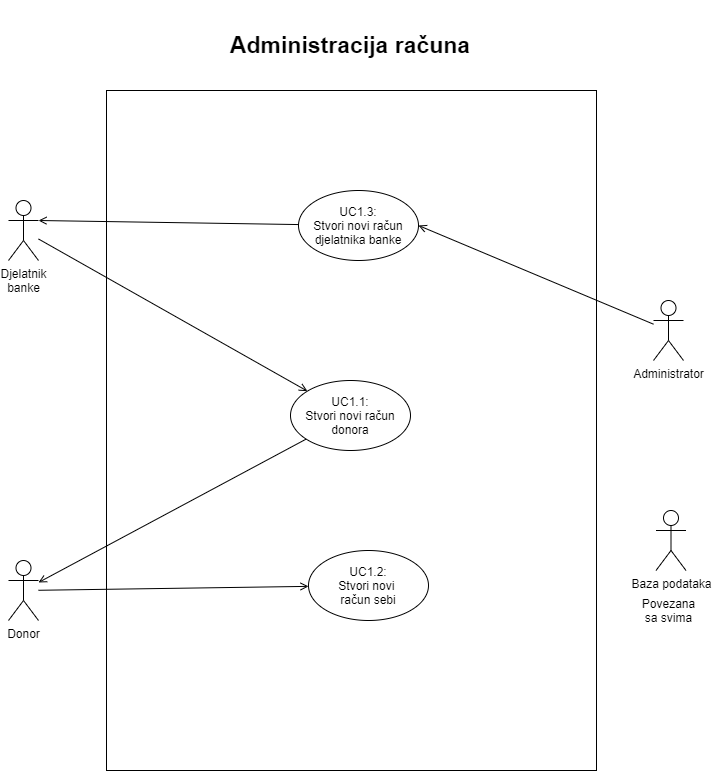
\includegraphics[scale=0.6]{slike/UC1.png} %veličina slike u odnosu na originalnu datoteku i pozicija slike
    			\centering
    			\caption{Dijagram obrazaca uporabe 1 - Administracija računa}
    			\label{fig:promjene}
    	    	\end{figure}
    	    	
				\begin{figure}[H]
    			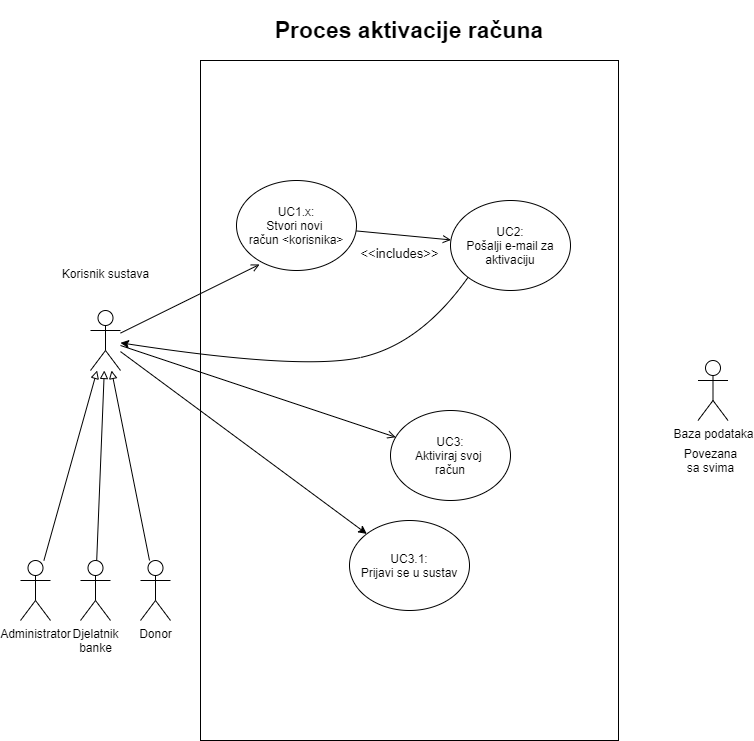
\includegraphics[scale=0.6]{slike/UC2.png} %veličina slike u odnosu na originalnu datoteku i pozicija slike
    			\centering
    			\caption{Dijagram obrazaca uporabe 2 - Proces aktivacije računa}
    			\label{fig:promjene}
    	    	\end{figure}
    	    	
				\begin{figure}[H]
    			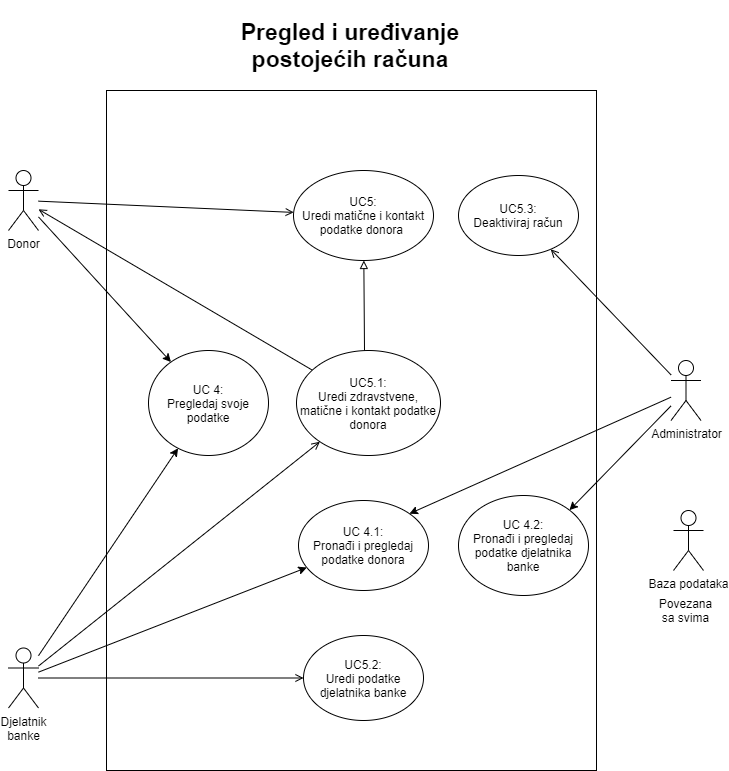
\includegraphics[scale=0.6]{slike/UC3.png} %veličina slike u odnosu na originalnu datoteku i pozicija slike
    			\centering
    			\caption{Dijagram obrazaca uporabe 3 - Uređivanje postojećih računa}
    			\label{fig:promjene}
    	    	\end{figure}
    	    	
				\begin{figure}[H]
    			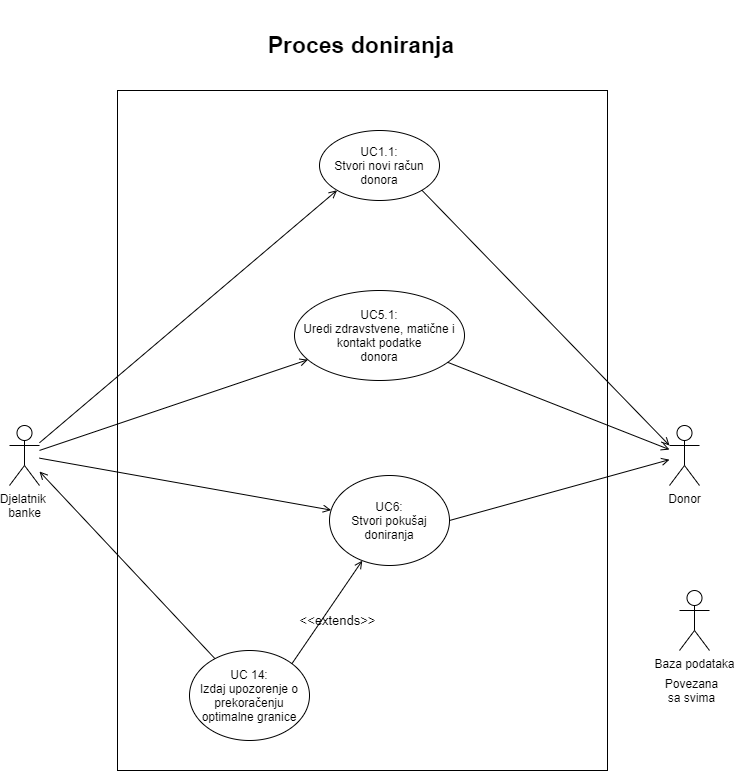
\includegraphics[scale=0.6]{slike/UC4.png} %veličina slike u odnosu na originalnu datoteku i pozicija slike
    			\centering
    			\caption{Dijagram obrazaca uporabe 4 - Proces doniranja}
    			\label{fig:promjene}
    	    	\end{figure}
    	    	
				\begin{figure}[H]
    			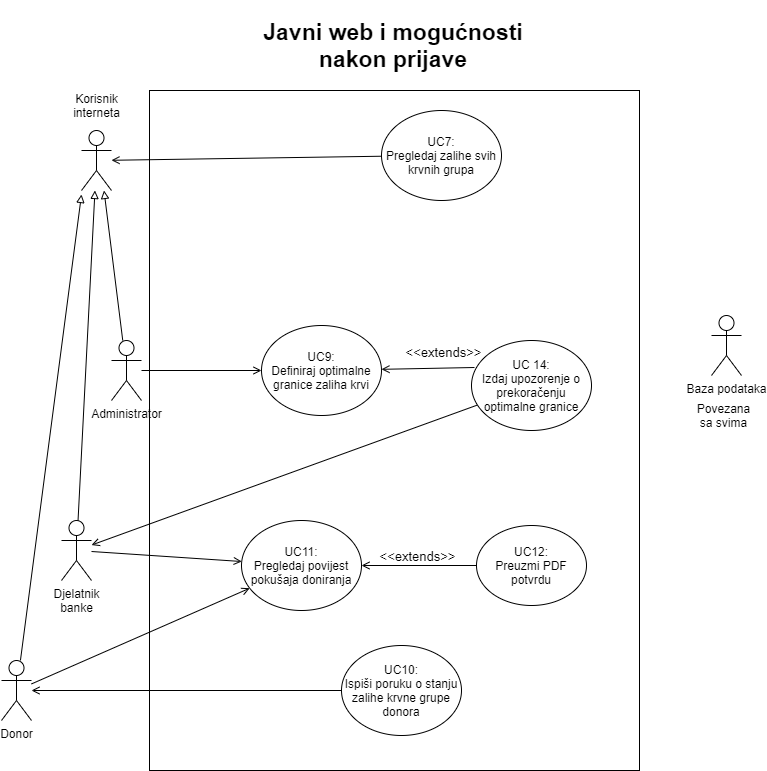
\includegraphics[scale=0.6]{slike/UC5.png} %veličina slike u odnosu na originalnu datoteku i pozicija slike
    			\centering
    			\caption{Dijagram obrazaca uporabe 5 - Javni web i mogućnosti nakon prijave}
    			\label{fig:promjene}
    	    	\end{figure}
    	    	
				\begin{figure}[H]
    			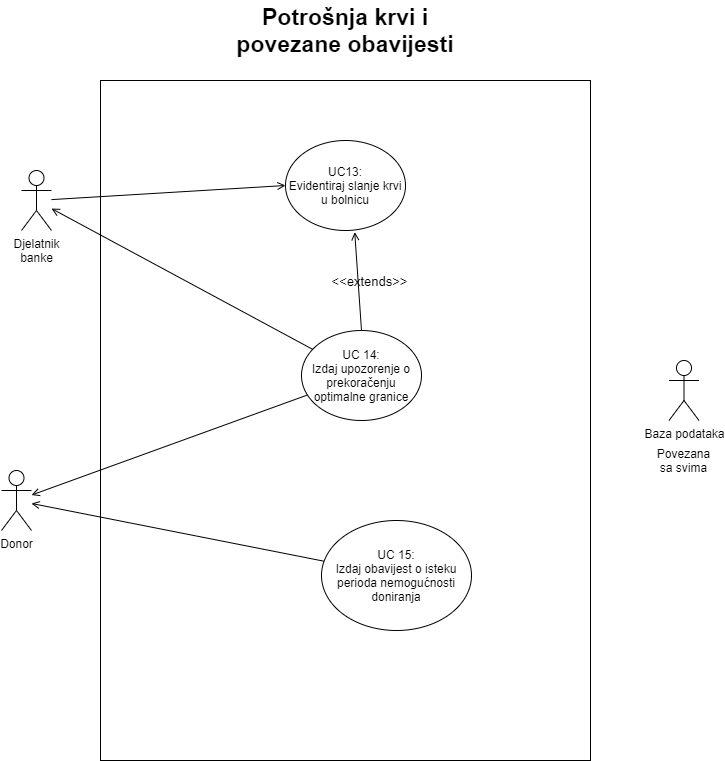
\includegraphics[scale=0.6]{slike/UC6.png} %veličina slike u odnosu na originalnu datoteku i pozicija slike
    			\centering
    			\caption{Dijagram obrazaca uporabe 6 - Potrošnja krvi i povezane obavijesti}
    			\label{fig:promjene}
    	    	\end{figure}
    	    	
				\eject		
				
			\subsection{Sekvencijski dijagrami}
				
				%\textbf{\textit{dio 1. revizije}}\\
				
				%\textit{Nacrtati sekvencijske dijagrame koji modeliraju najvažnije dijelove sustava (max. 4 dijagrama). Ukoliko postoji nedoumica oko odabira, razjasniti s asistentom. Uz svaki dijagram napisati detaljni opis dijagrama.}
				
				
				\begin{figure}[H]
    			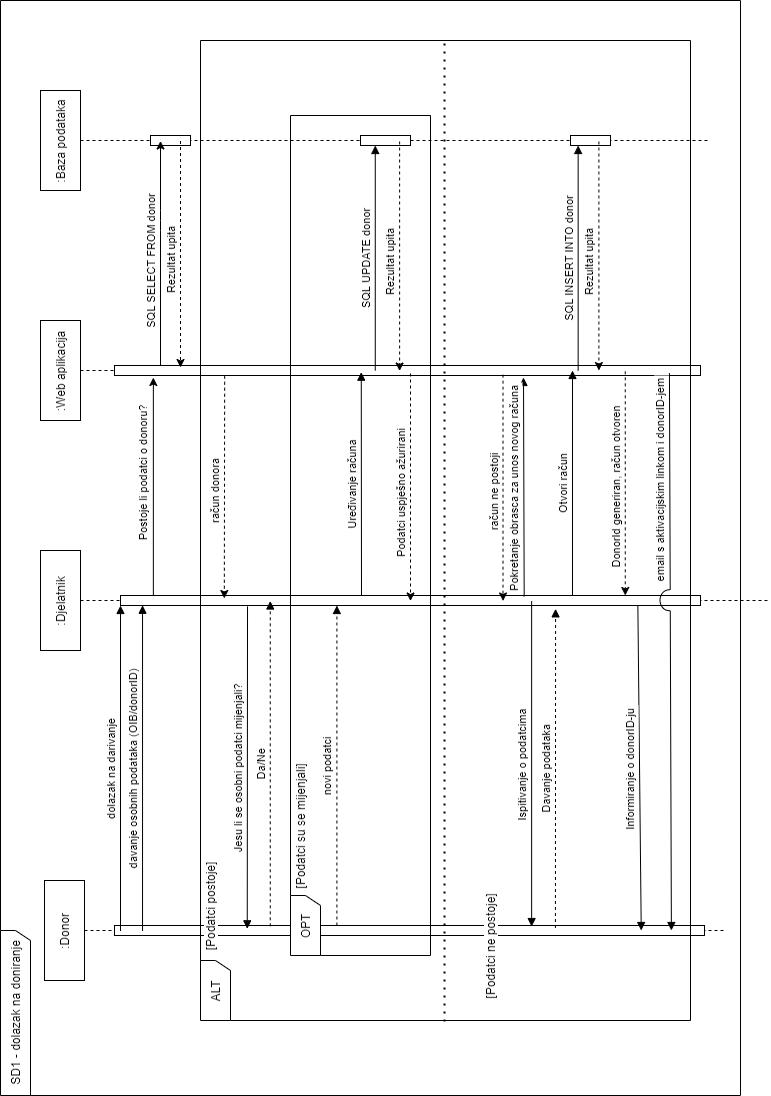
\includegraphics[scale=0.7]{slike/SD1_rot.png} %veličina slike u odnosu na originalnu datoteku i pozicija slike
    			\centering
    			\caption{Sekvencijski dijagram 1 - Potrošnja krvi i povezane obavijesti}
    			\label{fig:promjene}
    	    	\end{figure}
    	    	
    	    	\par {
    	    	    Sekvencijski dijagram 1: Donor dolazi na akciju darivanja krvi i djelatniku banke daje neki 
identifikacijski podatak (OIB ili donorID, ukoliko ga posjeduje).
Djelatnik banke provjerava postoji li u sustavu donor s tim podatkom (koji je
jedinstven za svaki račun). Web aplikacija djelatniku banke daje odgovor slanjem
upita u bazu podataka. Ukoliko podatci postoje, djelatnik banke u komunikaciji s 
donorom provjerava jesu li se podatci mijenjali i ažurira ih ako jesu.
U slučaju promjene, sustav ažurira podatke u bazi podataka.
Ukoliko nema postojećih podataka, sustav to dojavljuje djelatniku, koji kreće
u proces kreiranja novog računa. Djelatnik banke donora ispituje o osobnim podatcima,
unosi ih u sustav koji te podatke unosi u bazu podataka. Generira se donorID,
o kojemu djelatnik banke izvještava donora. Sustav također šalje e-mail s generiranim
podatcima o računu i poveznicom za aktivaciju računa.
    	    	}
    	    	
				\begin{figure}[H]
    			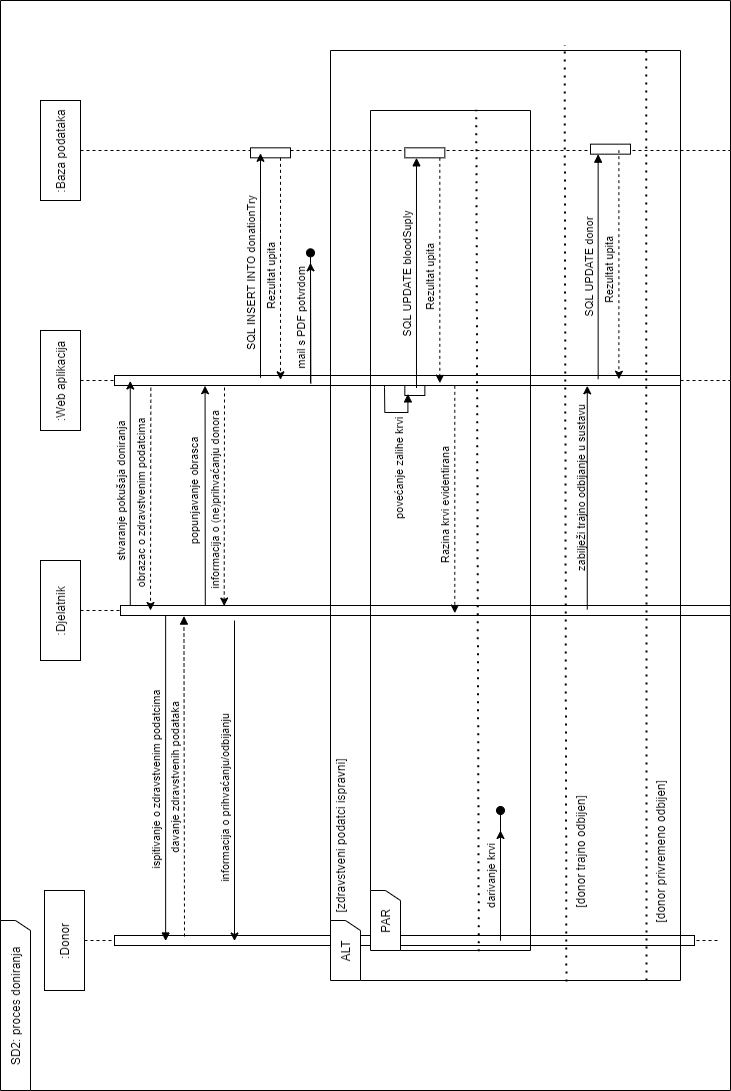
\includegraphics[scale=0.7]{slike/SD2_rot.png} %veličina slike u odnosu na originalnu datoteku i pozicija slike
    			\centering
    			\caption{Sekvencijski dijagram 2 - Potrošnja krvi i povezane obavijesti}
    			\label{fig:promjene}
    	    	\end{figure}
				
				\eject
				
				\par {
    	    	   Sekvencijski dijagram 2: Nakon provjere postojanja i ispravnosti podataka u sustavu, djelatnik banke za
donora stvara pokušaj doniranja. U obrazac koji se otvara u web aplikaciji
djelatnik banke evidentira zdravstvene podatke koje otkriva u komunikaciji s 
donorom (ili iz popunjenog obrasca koji mu dostavi donor).
Ukoliko neki od podataka implicira nemogućnost donora za darivanje krvi,
djelatnik banke donora informira o tome. Pokušaj doniranja sprema se u bazu podataka
te se donoru na mail šalje potvrda o pokušaju doniranja.
U slučaju da je donor nije odbijen (zdravstveni podatci su ispravni), u
sustavu se povećava zaliha krvi za jednu dozu ažuriranjem podataka u bazi, a
donor odlazi donirati krv.
U slučaju da je donor trajno odbijen, djelatnik banke dodatno u njegovom računu zabilježava
trajno odbijanje ažuriranjem donorovih podataka u bazi.
Ako je donor samo privremeno odbijen, ne poduzimaju se nikakvi dodatni koraci.
    	    	}
				
				
				
	
		\section{Ostali zahtjevi}
		
			%\textbf{\textit{dio 1. revizije}}\\
		 
			 %\textit{Nefunkcionalni zahtjevi i zahtjevi domene primjene dopunjuju funkcionalne zahtjeve. Oni opisuju \textbf{kako se sustav treba ponašati} i koja \textbf{ograničenja} treba poštivati (performanse, korisničko iskustvo, pouzdanost, standardi kvalitete, sigurnost...). Primjeri takvih zahtjeva u Vašem projektu mogu biti: podržani jezici korisničkog sučelja, vrijeme odziva, najveći mogući podržani broj korisnika, podržane web/mobilne platforme, razina zaštite (protokoli komunikacije, kriptiranje...)... Svaki takav zahtjev potrebno je navesti u jednoj ili dvije rečenice.}
			 
			 \begin{itemize}
			     \item Sustav treba omogućiti rad više korisnika
			     \item U sustavu treba postojati tri vrste korisnika - donor, djelatnik banke i administrator
			     \item Aplikacija mora biti izvedena kao web-aplikacija
			     \item Aplikacija mora biti prilagodljiva različitim veličinama ekrana te mobilnim uređajima
			     \item Autentikacija korisnika radi se korisničkim imenom (donorID) i lozinkom
			     \item Lozinke u sustavu moraju biti enkriptirane radi zaštite u slučaju neovlaštenog pristupa
			     \item Lozinke korisnika moraju biti dovoljno sigurne radi sprječavanja neovlaštenog pristupa računu (trebaju imati bar 2 od 4 zahtjeva - mala slova, velika slova, brojevi, specijalni znakovi) 
			     \item Računi su pri stvaranju neaktivirani, a aktiviraju se aktivacijskim linkom dostavljenim u e-mailu koji se šalje pri kreiranju računa na e-adresu navedenu pri kreiranju računa
			     \item Sustav korisnicima ne smije otežavati rad, stoga mora biti napravljen intuitivno i kao jednostavan za korištenje
			     \item Sustav mora biti otporan na pogreške, ne smije se srušiti, nego treba dojaviti pogrešku i omogućiti izmjenu neispravno unesenih podataka
			 \end{itemize}
			 
			 
			 
	
	\chapter{Arhitektura i dizajn sustava} \label{arhitektura}
		
%		\textbf{\textit{dio 1. revizije}}\\
		
%		\textit{ Potrebno je opisati stil arhitekture te identificirati: podsustave, preslikavanje na radnu platformu, spremišta podataka, mrežne protokole, globalni upravljački tok i sklopovsko-programske zahtjeve. Po točkama razraditi i popratiti odgovarajućim skicama:}

%	\begin{itemize}
%		\item 	\textit{izbor arhitekture temeljem principa oblikovanja pokazanih na predavanjima (objasniti zašto ste baš odabrali takvu arhitekturu)}
%		\item 	\textit{organizaciju sustava s najviše razine apstrakcije (npr. klijent-poslužitelj, baza podataka, datotečni sustav, grafičko sučelje)}
%		\item 	\textit{organizaciju aplikacije (npr. slojevi frontend i backend, MVC arhitektura) }		
%	\end{itemize}



%   OVDJE PIŠE ŠTO TREBA NAPISATI!---^^^
		
    \noindent { Arhitektura se može podijeliti na tri podsustava:}
	\begin{itemize}
		\item{Web poslužitelj}
		\item{Web aplikacija}
		\item{Baza podataka}		
	\end{itemize}
	
	\underline{\textit{Web poslužitelj}} osnova je rada web aplikacije. Njegova primarna zadaća je komunikacija klijenta s aplikacijom. Komunikacija se odvija preko HTTP (engl. Hyper Text Transfer Protocol) protokola, što je protokol u prijenosu informacija na webu. Poslužitelj je onaj koji pokreće web aplikaciju te joj prosljeđuje zahtjev.
	
	Korisnik koristi \underline{\textit{web aplikaciju}} za obrađivanje željenih zahtijeva. Web aplikacija obrađuje zahtjev te ovisno o zahtjevu, pristupa bazi podataka, vraća web-poslužitelju odgovor u JSON formatu, a zatim web poslužitelj te informacije prikazuje na svoj način.
		\begin{figure}[H]
                    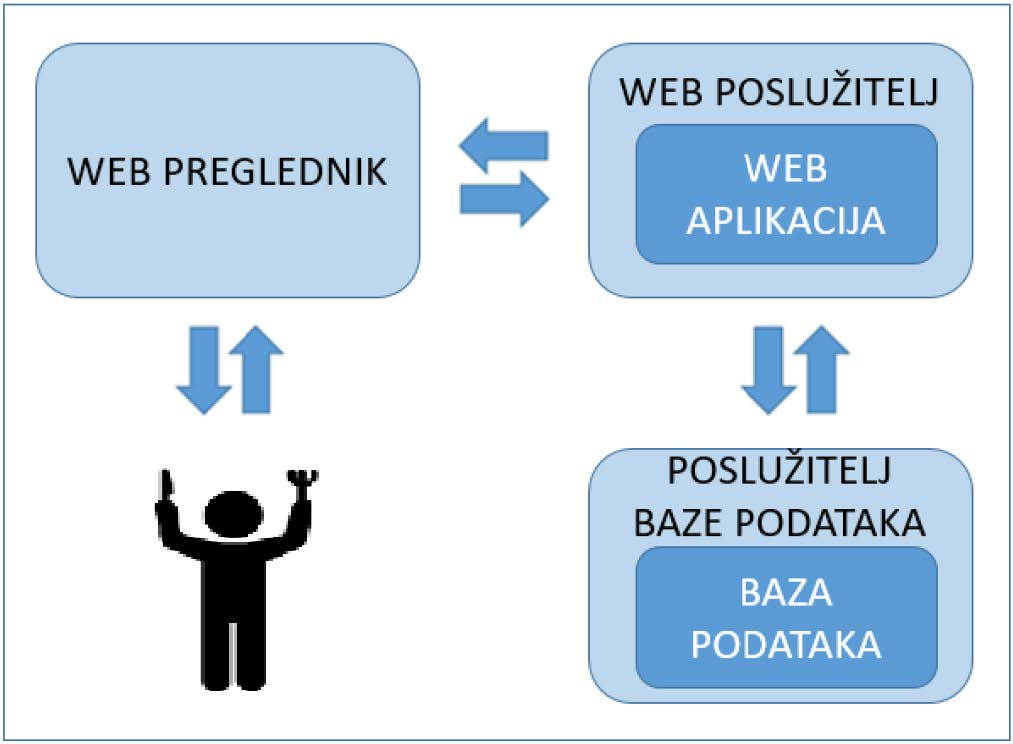
\includegraphics[scale=1]{slike/Arhitektura sustava.jpg}
        			\centering
        			\caption{Arhitektura sustava}
        			\label{fig:hztm-stranica}
        		\end{figure}
			
			\eject

	Programski jezik koji smo odabrali za izradu naše web aplikacije je Java zajedno sa SpringBoot radnim okvirom te programski jezik Javascript s React bibliotekom (eng. library). Odabrano razvojno okruženje je IntelliJ. 
	
	Arhitektura sustava sastoji se od 3 razine:
	\begin{itemize}
		\item{\textbf{Sučelje} - Najviša razina aplikacije, glavna funkcija sučelja je prevesti procese i rezultate u format koji korisnik može razumijeti}
		\item{\textbf{Logika} - Ova razina koordinira aplikaciju, obrađuje naredbe, izvršava logiku i računa. Također prenosi podatke između podatkovne razine i sučelja.}
		\item{\textbf{Podatci} - Ova razina uključuje spremanje i dohvaćanje podatke iz baze podataka}		
	\end{itemize}
	
	Funkcionalnosti aplikacije se izvršavaju slanjem upita na \textit{\underline{endpointe}}. Oni definiraju adresu ili točku spajanja na Web poslužitelj. Tipično je reprezentiran jednostavnim HTTP URL-om (adresom, \textit{linkom}).
	
	Implementirani Endpointi su:
	\begin{itemize}
	    \item {\textbf{Prijava} - Omogućava pristup korisničkom računu, provjerava jeli dobro postavljen session cookie}
	    \item {\textbf{Kreiranje donora od strane donora}}
	    \item {\textbf{Kreiranje donora od strane radnika}}
	    \item {\textbf{Prikaz korisničkih podataka}}
	\end{itemize}

	

	
		

		

				
		\section{Baza podataka}
			
%			\textbf{\textit{dio 1. revizije}}\\
			
		Sustav koristi relacijsku bazu podataka. Relacijske baze podataka pohranjuju i pružaju pristup podatcima. Gradivna jedinka baze je relacija, odnosno tablica koja je definirana svojim imenom i skupom atributa. Prednost relacijskih baza jest lakše definiranje odnosa između podataka. Baza podataka ove aplikacije sastoji se od ovih entiteta:
		\begin{itemize}
	        \item Korisnik
	        
	        \begin{itemize}
	            \item Donor krvi
	            \item Djelatnik banke
	        \end{itemize}
	        
	        \item Zaliha krvi
	        \item Pokušaj donacije
	        
	        
	    \end{itemize}
		
		
			\subsection{Opis tablica}
			

		%		\textit{Svaku tablicu je potrebno opisati po zadanom predlošku. Lijevo se nalazi točno ime varijable u bazi podataka, u sredini se nalazi tip podataka, a desno se nalazi opis varijable. Svjetlo zelenom bojom označen je primarni ključ. Svjetlo plavom označen je strani ključ. Svijetlo tirkiznom bojom označen je ključ koji je primarni i strani. Svijetlo crvenom bojom označeni su unique atributi koji nisu ključevi.}
				
				
				
				
			% OVO STAVI KAO NASLOV SVAKE TABLICE U OVE PRVE UGLATE ZAGRADE, GDJE PIŠE LABEL=NONE (mozes vidjeti primjer kod dnevnika promjena)
			%caption = {Dnevnik promjena dokumentacije}
			
		\textbf{Korisnik} - Ovaj entitet sadržava sve administrativne podatke o korisniku aplikacije, njegovi osnovni podatci nalaze se u drugim, personiliziranim entitetima. Sadrži atribute: user id, user role, password, acc activated, perm deactivated, opt out. Ovaj entitet u vezi je \textit{One-to-one} sa entitetima Donorom i Djelatnikom banke preko atributa donor id, odnosno bank worker id. 
			
				\begin{longtblr}[
				    caption = {Tablica \textit{korisnik} u bazi podataka},
					label=none
					]{
						width = \textwidth,
						colspec={|X[6,l]|X[7, l]|X[20, l]|}, 
						rowhead = 1,
					} %definicija širine tablice, širine stupaca, poravnanje i broja redaka naslova tablice
					\hline \multicolumn{3}{|c|}{\textbf{Korisnik}}	 \\ \hline[3pt]
					\SetCell{LightGreen}user id & BIGINT	&  	Jedinstveni identifikator korisnika  	\\ \hline
					user role	& VARCHAR(20) &  Je li korisnik donor, djelatnik  banke ili administrator 	\\ \hline 
					password & VARCHAR(128) &  Enkriptirana lozinka korisnika \\ \hline 
					acc activated & INT	& Je li korisnik preko e-maila aktivirao svoj račun  		\\ \hline 
					perm deactivated & INT &  Je li korisnički račun trajno dekativiran \\ \hline 
					opt out & INT &  Je li uključena opcija koja isključuje notifikacije \\ \hline 
				\end{longtblr}
				
				
		\textbf{Donor} - Ovaj entitet sadržava osobne podatke o korisniku aplikacije koji je donor. Sadrži atribute: donor id, first name, last name, oib, birth date, birth place, address, work place, private contact, work contact, email, blood type. Ovaj entitet u vezi je \textit{One-to-many} sa entitetom Pokušaj donacije preko atributa donor id. Također je u vezi \textit{One-to-one} sa entitetom Korisnik preko atributa donor id.
				
				\begin{longtblr}[
				    caption = {Tablica \textit{donor} u bazi podataka},
					label=none
					]{
						width = \textwidth,
						colspec={|X[6,l]|X[7, l]|X[20, l]|}, 
						rowhead = 1,
					} %definicija širine tablice, širine stupaca, poravnanje i broja redaka naslova tablice
					\hline \multicolumn{3}{|c|}{\textbf{Donor}}	 \\ \hline[3pt]
					\SetCell{LightTeal}donor id & BIGINT	&  	Jedinstveni identifikator donora krvi, odgovara identifikatoru korisnika  	\\ \hline
					first name	& VARCHAR(50) &  Ime donora krvi 	\\ \hline 
					last name & VARCHAR(50) &  Prezime donora krvi \\ \hline 
					\SetCell{LightRed}oib & CHAR(11)	& OIB donora krvi  		\\ \hline 
					birth date & DATE &  Datum rođenja donora krvi \\ \hline 
					birth place & VARCHAR(100) &  Mjesto rođenja donora krvi \\ \hline 
					address & VARCHAR(100)	& Adresa stanovanja donora krvi  		\\ \hline 
					work place & VARCHAR(100) &  Mjesto zaposlenja donora krvi \\ \hline 
					private contact & VARCHAR(20) &  Osobni kontakt broj mobitela donora krvi \\ \hline 
					work contact & VARCHAR(20) &  Poslovni kontakt broj mobitela donora krvi \\ \hline 
					email & VARCHAR(50) &  e-mail adresa donora krvi \\ \hline 
					\SetCell{LightBlue}blood type & VARCHAR(3) &  Krvna grupa donora krvi \\ \hline 
					perm rejected reason & VARCHAR(100) &  Ako je račun donora krvi trajno deaktiviran, razlog deaktivacije \\ \hline
				\end{longtblr}
				
		\textbf{Djelatnik banke} - Ovaj entitet sadržava osobne podatke djelatnika banke. Sadrži atribute: bank worker id, first name, last name, oib, birth date, birth place, address, work place, private contact, work contact, email. U vezi je \textit{One-to-one} sa entitetom Korisnik preko atributa bank worker id.
				
				\begin{longtblr}[
				    caption = {Tablica \textit{djelatnik banke} u bazi podataka},
					label=none
					]{
						width = \textwidth,
						colspec={|X[6,l]|X[7, l]|X[20, l]|}, 
						rowhead = 1,
					} %definicija širine tablice, širine stupaca, poravnanje i broja redaka naslova tablice
					\hline \multicolumn{3}{|c|}{\textbf{Djelatnik banke}}	 \\ \hline[3pt]
					\SetCell{LightTeal}bank worker id & BIGINT	&  	Jedinstveni identifikator djelatnika banke, odgovara identifikatoru korisnika  	\\ \hline
					first name	& VARCHAR(50) &  Ime djelatnika banke  	\\ \hline 
					last name & VARCHAR(50) &  Prezime djelatnika banke  \\ \hline 
					\SetCell{LightRed}oib & CHAR(11)	& OIB djelatnika banke   		\\ \hline 
					birth date & DATE &  Datum rođenja djelatnika banke  \\ \hline 
					birth place & VARCHAR(100) &  Mjesto rođenja djelatnika banke  \\ \hline 
					address & VARCHAR(100)	& Adresa stanovanja djelatnika banke  		\\ \hline 
					work place & VARCHAR(100) &  Mjesto zaposlenja djelatnika banke  \\ \hline 
					private contact & VARCHAR(20) &  Osobni kontakt broj mobitela djelatnika banke  \\ \hline
					work contact & VARCHAR(20) &  Poslovni kontakt broj mobitela djelatnika banke  \\ \hline 
					email & VARCHAR(50) &  e-mail adresa djelatnika banke  \\ \hline 
				\end{longtblr}
				
		\textbf{Zaliha krvi} - Ovaj entitet sadržava podatke o količini krvi u banci. Sadrži atribute: number of units, max units, min units.
			
				\begin{longtblr}[
				    caption = {Tablica \textit{zaliha krvi} u bazi podataka},
					label=none
					]{
						width = \textwidth,
						colspec={|X[6,l]|X[6, l]|X[20, l]|}, 
						rowhead = 1,
					} %definicija širine tablice, širine stupaca, poravnanje i broja redaka naslova tablice
					\hline \multicolumn{3}{|c|}{\textbf{Zaliha krvi}}	 \\ \hline[3pt]
					\SetCell{LightGreen}blood type & CHAR(3) & Krvna grupa jedinice krvi \\ \hline
					number of units	& INT &  Trenutni broj jedinica krvi  	\\ \hline 
					max units & INT &  Maksimalni broj jedinica krvi \\ \hline 
					min units & INT	& Minimalni broj jedinica krvi \\ \hline 
				\end{longtblr}
				
		\textbf{Pokušaj donacije} - Ovaj entitet sadržava podatke o pojedinoj donaciji krvi. Sadrži atribute: donation id, rejected reason, blood type, donor id, bank worker id. U vezi je \textit{Many-to-one} sa entitetom Donor preko atributa donor id.
		        
				\begin{longtblr}[
				    caption = {Tablica \textit{pokušaj donacije} u bazi podataka},
					label=none
					]{
						width = \textwidth,
						colspec={|X[6,l]|X[7, l]|X[20, l]|}, 
						rowhead = 1,
					} %definicija širine tablice, širine stupaca, poravnanje i broja redaka naslova tablice
					\hline \multicolumn{3}{|c|}{\textbf{Pokušaj donacije}}	 \\ \hline[3pt]
					rejected reason	& VARCHAR(100) &  Razlog neuspješnosti pokušaja darivanja krvi 	\\ \hline 
					\SetCell{LightBlue}blood type & CHAR(3) &  Kvrna grupa donora krvi koji obavlja ovu donaciju \\ \hline 
					\SetCell{LightBlue}donor id & BIGINT	& Jedinstveni identifikator donora krvi koji obavlja ovu donaciju krvi \\ \hline 
					\SetCell{LightBlue}bank worker id & BIGINT	& Jedinstveni identifikator djelatnika banke koji nadgleda ovu donaciju krvi \\ \hline 
				\end{longtblr}
				
				
			
			\subsection{Dijagram baze podataka}
			
				
				\begin{figure}[H]
                    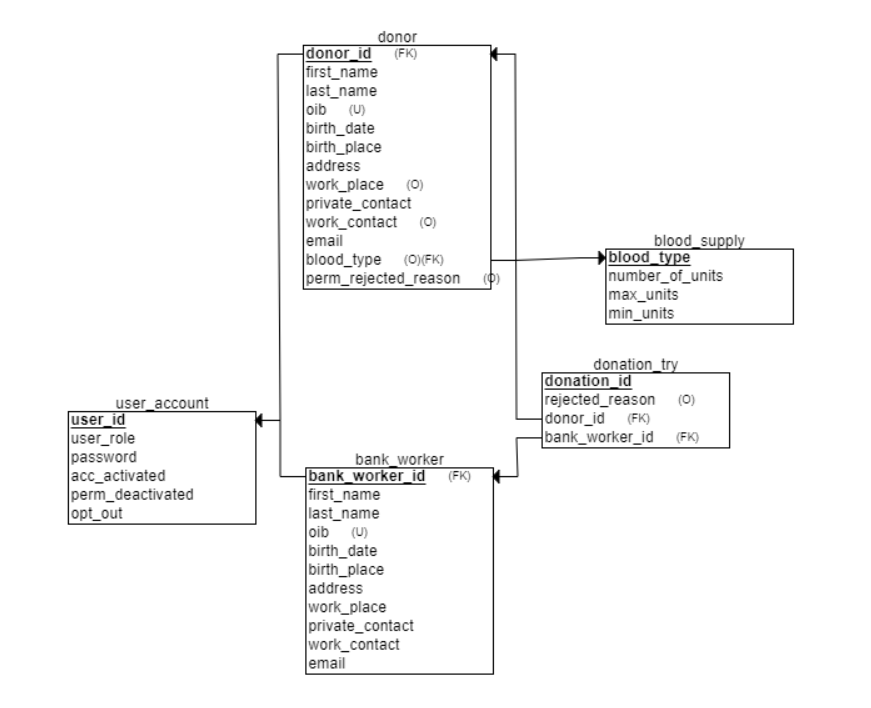
\includegraphics[scale=0.9]{slike/relational schema.png}
        			\centering
        			\caption{Relacijska shema baze podataka}
        			\label{fig:hztm-stranica}
        		\end{figure}
			
			\eject
			
			
		\section{Dijagram razreda}
		
%			\textit{Potrebno je priložiti dijagram razreda s pripadajućim opisom. Zbog preglednosti je moguće dijagram razlomiti na više njih, ali moraju biti grupirani prema sličnim razinama apstrakcije i srodnim funkcionalnostima.}\\
			
			\textbf{\textit{dio 1. revizije}}\\
			
%			\textit{Prilikom prve predaje projekta, potrebno je priložiti potpuno razrađen dijagram razreda vezan uz \textbf{generičku funkcionalnost} sustava. Ostale funkcionalnosti trebaju biti idejno razrađene u dijagramu sa sljedećim komponentama: nazivi razreda, nazivi metoda i vrste pristupa metodama (npr. javni, zaštićeni), nazivi atributa razreda, veze i odnosi između razreda.}\\

Na slikama u nastavku prikazani su razredi koji pripadaju "backend" dijelu arhitekture. Slike su podlijeljene po pripadnosti odgovarajćim entitetima iz baze podataka koji su opisani u poglavlju 4.1 (Baza podataka). Za svaki entitet postoje klase sljedećih tipova:
\begin{itemize}
	        \item \textbf{Controller} - Vraća "response entity" objekt koji sadrži http status i .json objekt na endpoint-e. Obično se radi o vraćanju podataka iz baze podataka. Controller također određuje korisničke dozvole pristupa pojedinim endpoint-ima  .
	        \item \textbf{Service} - Obavlja poslovnu logiku aplikacije. To uključuje validaciju računa, kreiranje računa, provjeru podataka itd.
	        \item \textbf{Repository} - Vadi i sprema podatke iz baze podataka, koristeći Spring Data JPA.
	        \item \textbf{Model} - Objekt koji je mapiran na entitet iz baze podataka. Sadrži atribute i konstruktore te gettere i settere.
	    \end{itemize}
	    
Neki entiteti imaju DTO metode koje služe kako bi se mogao vratiti samo dio podataka pomoću Controller-a na endpoint.
	    

                \begin{figure}[H]
                    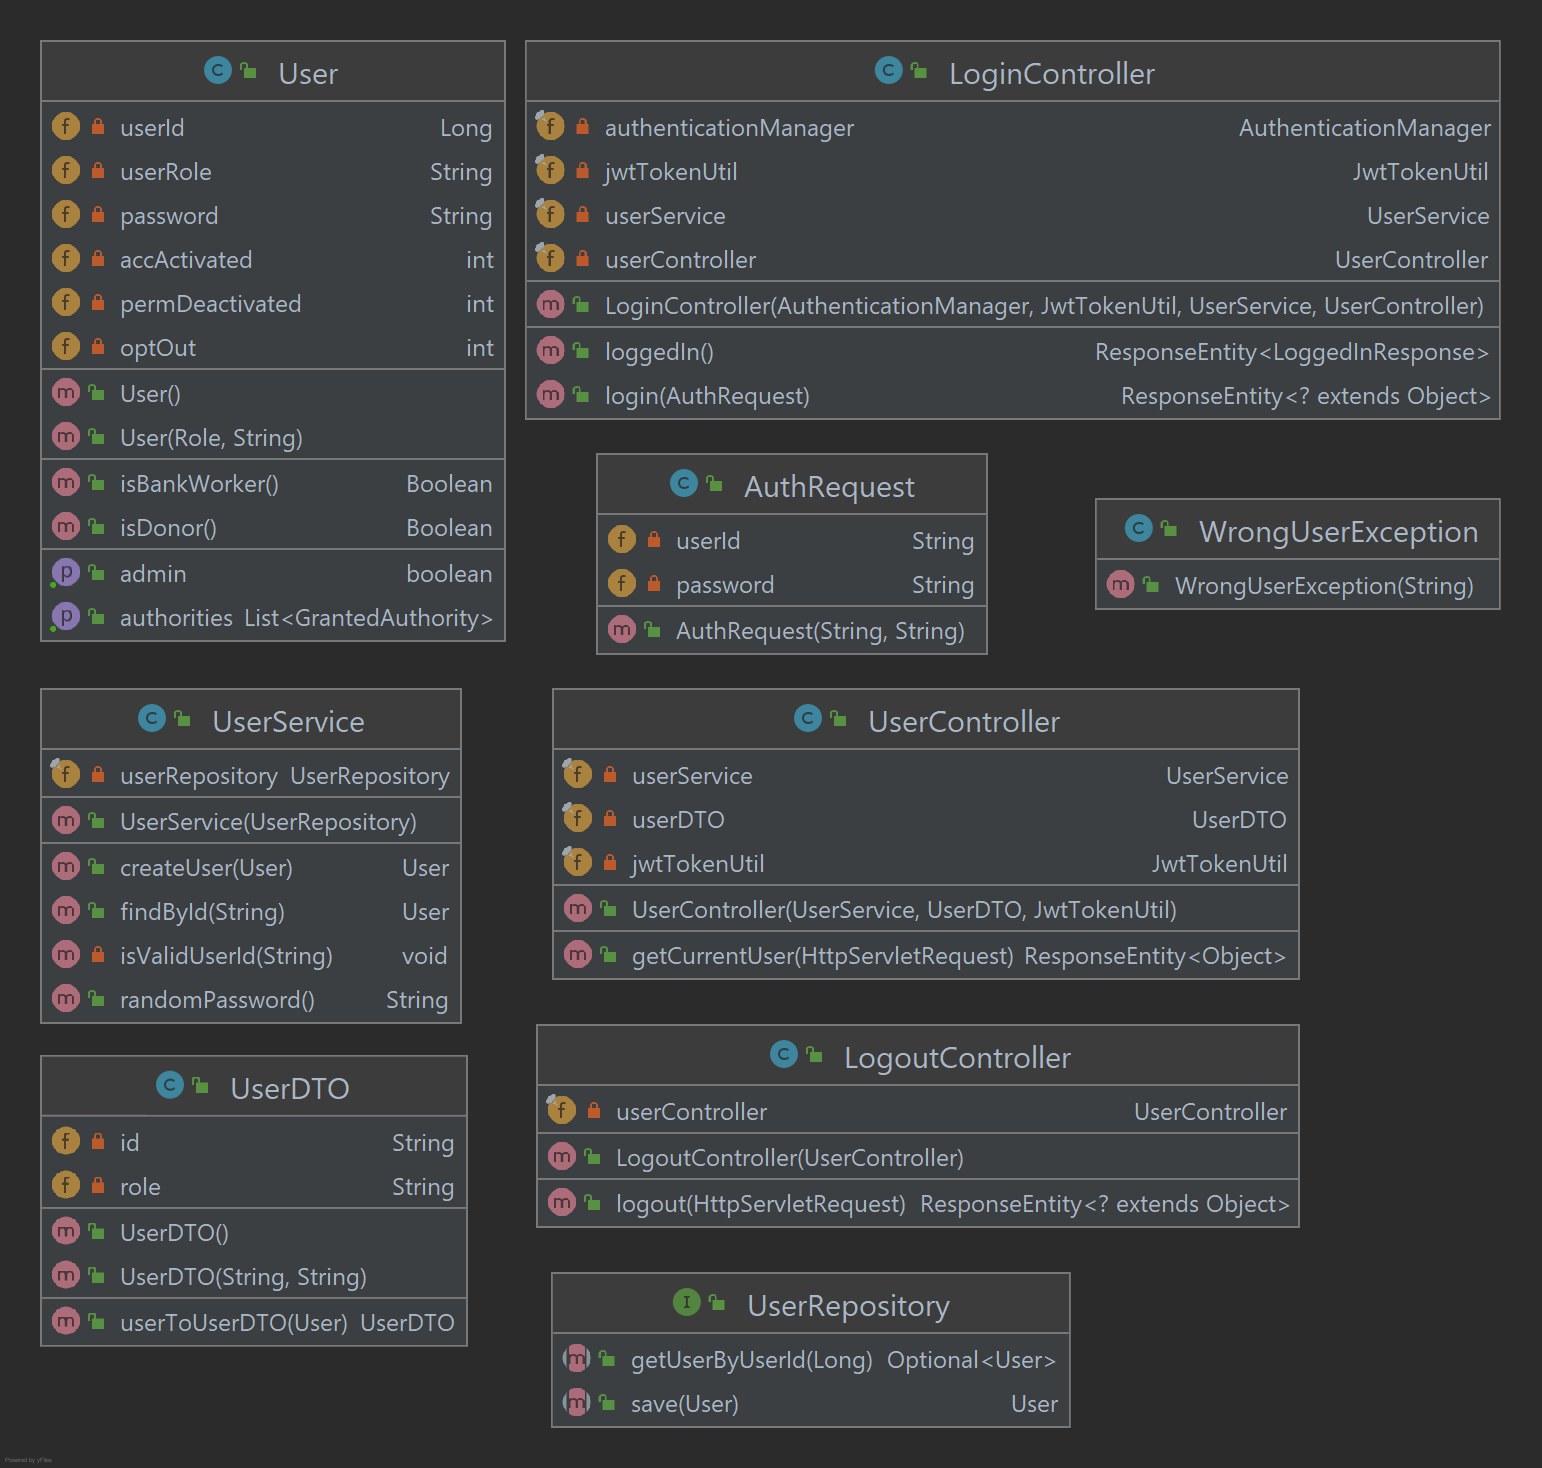
\includegraphics[scale=0.28]{slike/user.png}
        			\centering
        			\caption{Dijagram razreda vezanih za entitet Korisnik}
        			\label{fig:hztm-stranica}
        		\end{figure}

Entitetu Korisnik pripadaju klase LoginController i LogoutController.

LoginController je zadužen za ostvarivanje funkcionalnosti prijave. Lozinke se spremaju i provjeravaju u kodiranom obliku pomoću BCryptEncoder-a]. Dakle, koristi se sigurnosna shema Bearer Authentication.

LogoutController je zadužen za odjavu korisnika.

Entiteti Korisnik i Donor mogu uzrokovati iznimke ako se radi o krivom korisniku/donoru.

                \begin{figure}[H]
                    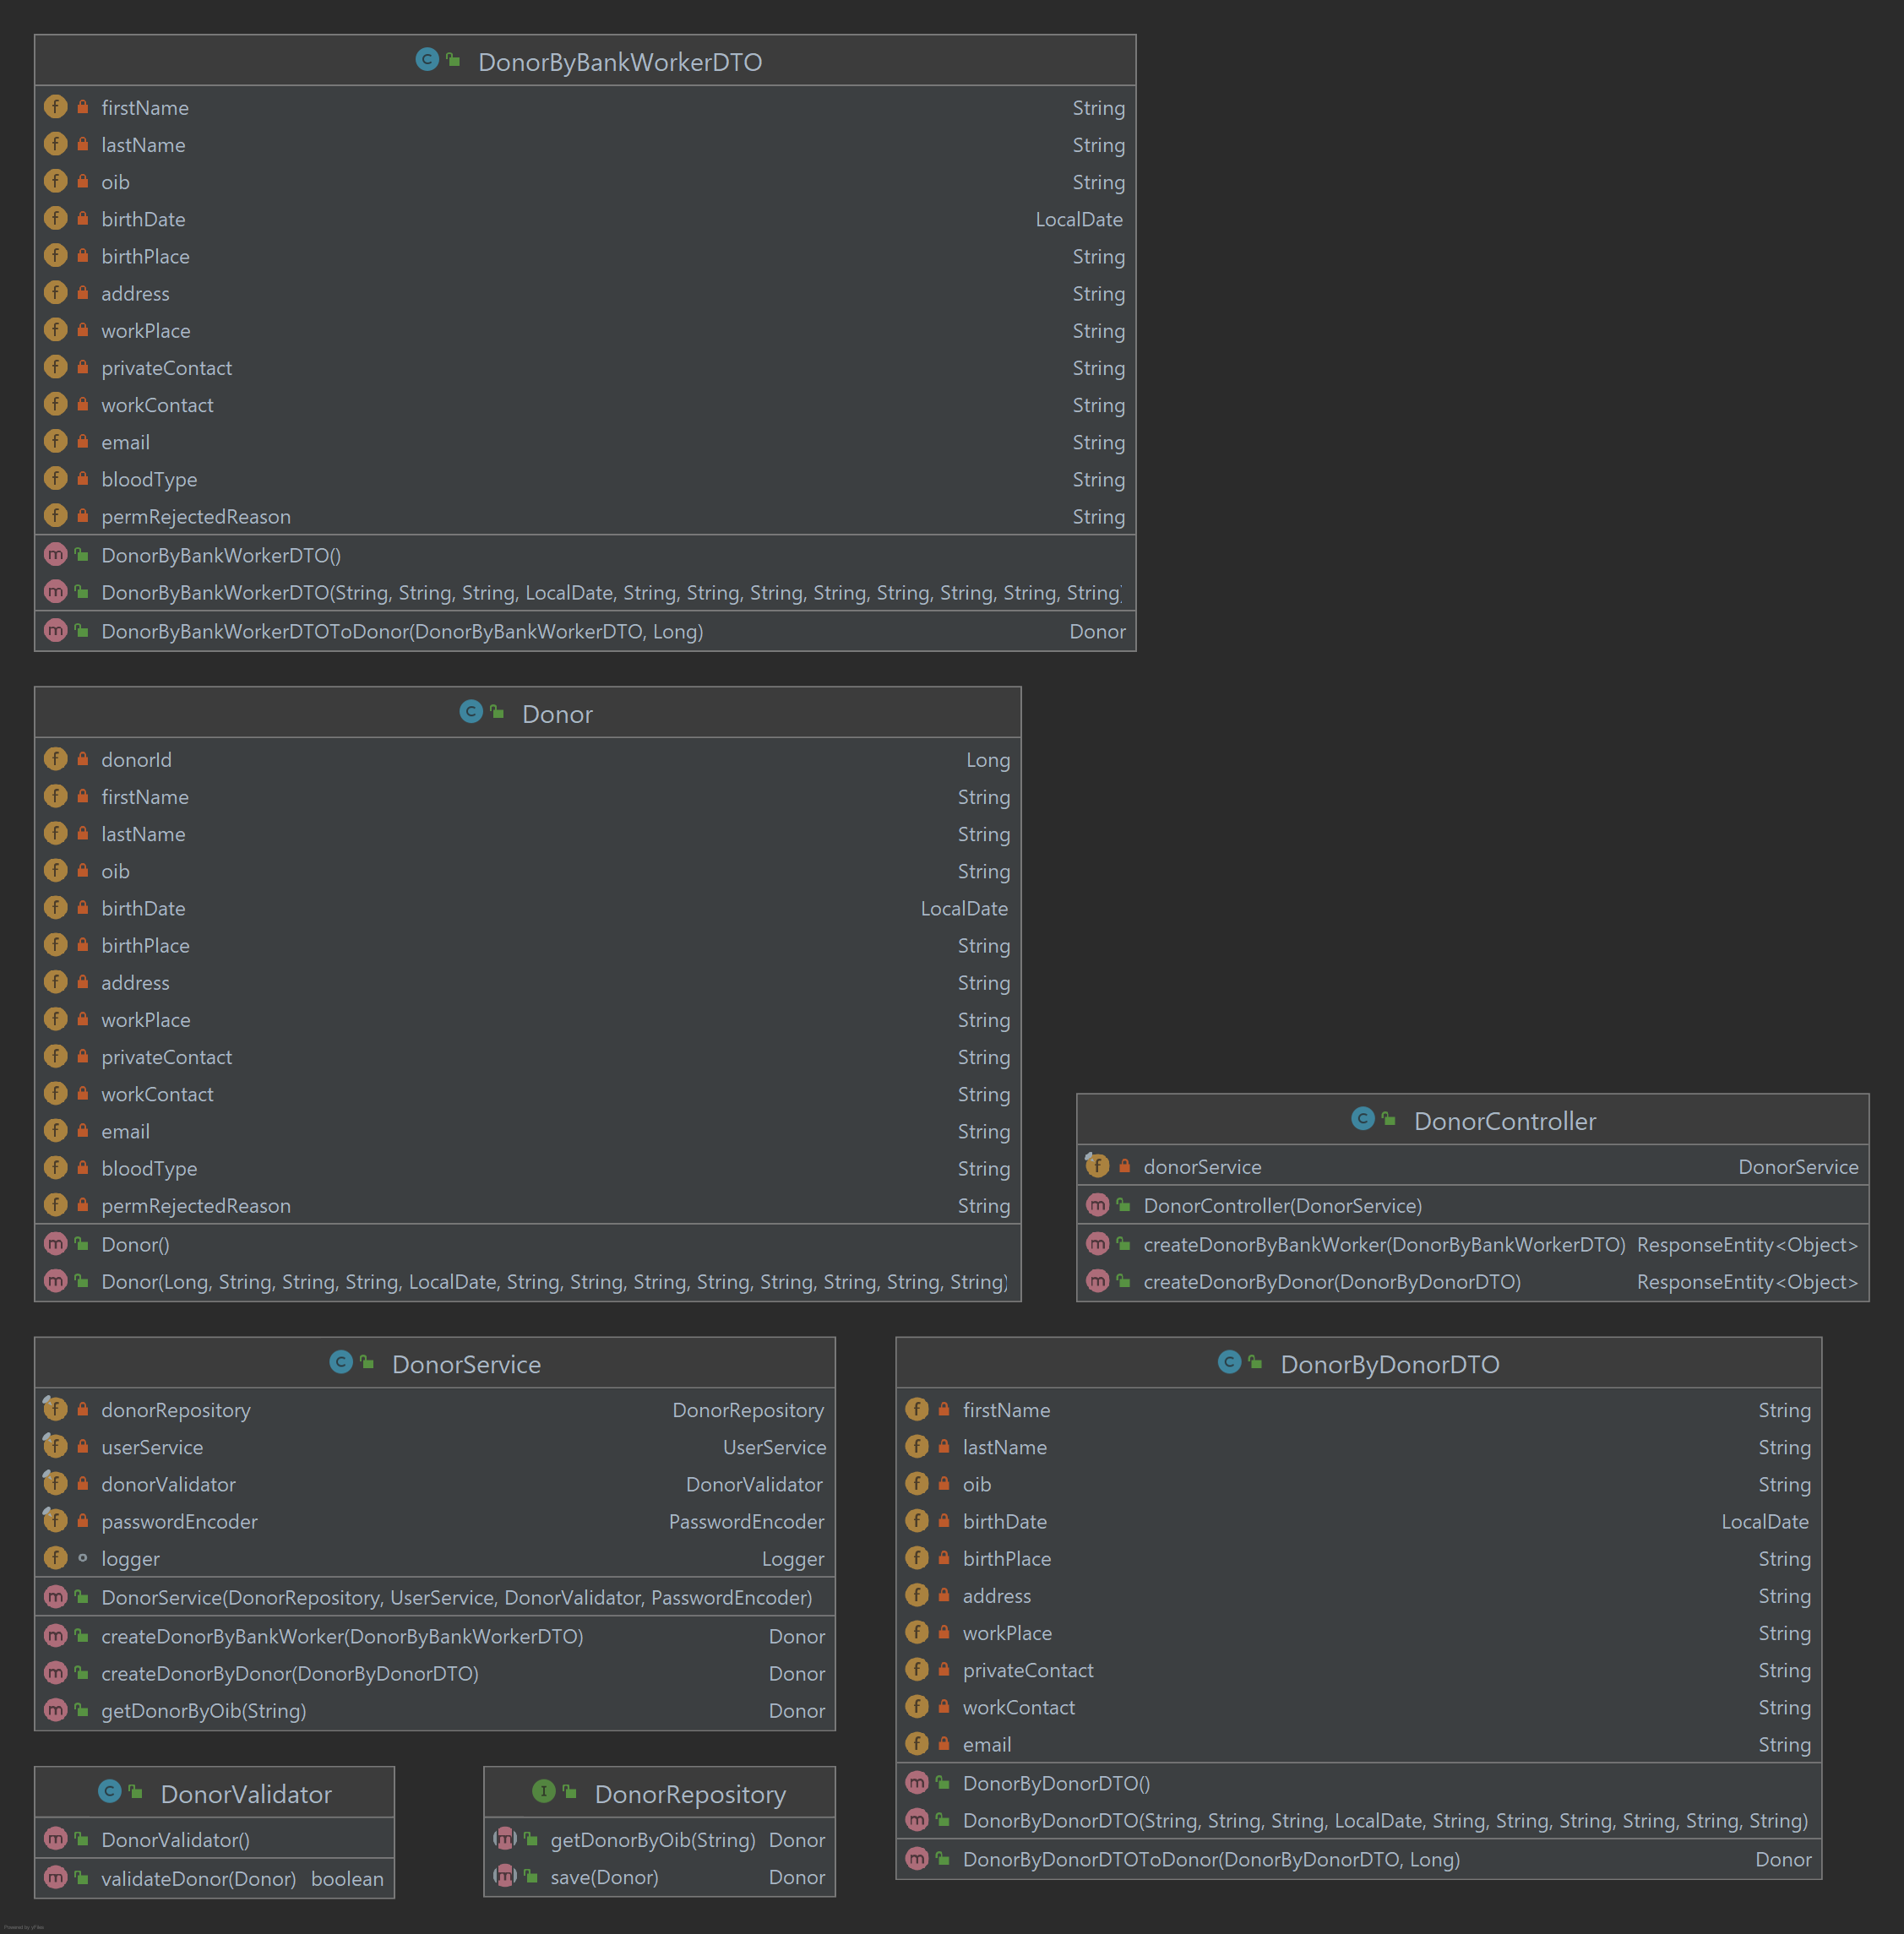
\includegraphics[scale=0.20]{slike/donor.png}
        			\centering
        			\caption{Dijagram razreda vezanih za entitet Donor}
        			\label{fig:hztm-stranica}
        		\end{figure}
        		
        		\begin{figure}[H]
                    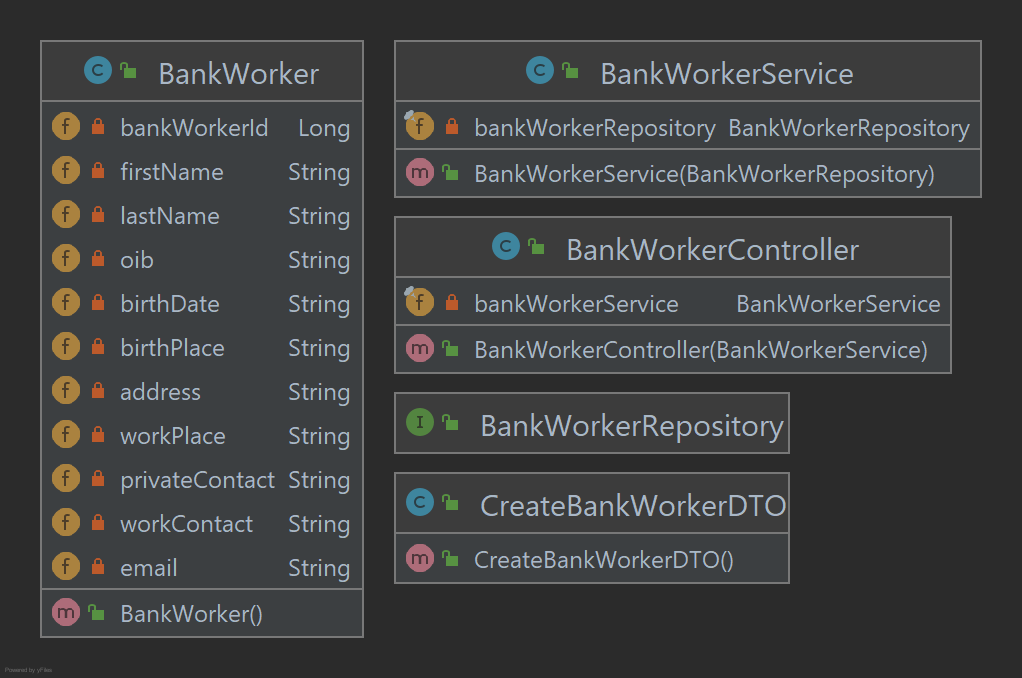
\includegraphics[scale=0.25]{slike/bankworker.png}
        			\centering
        			\caption{Dijagram razreda vezanih za entitet Djelatnika banke}
        			\label{fig:hztm-stranica}
        		\end{figure}
        		
        		\begin{figure}[H]
                    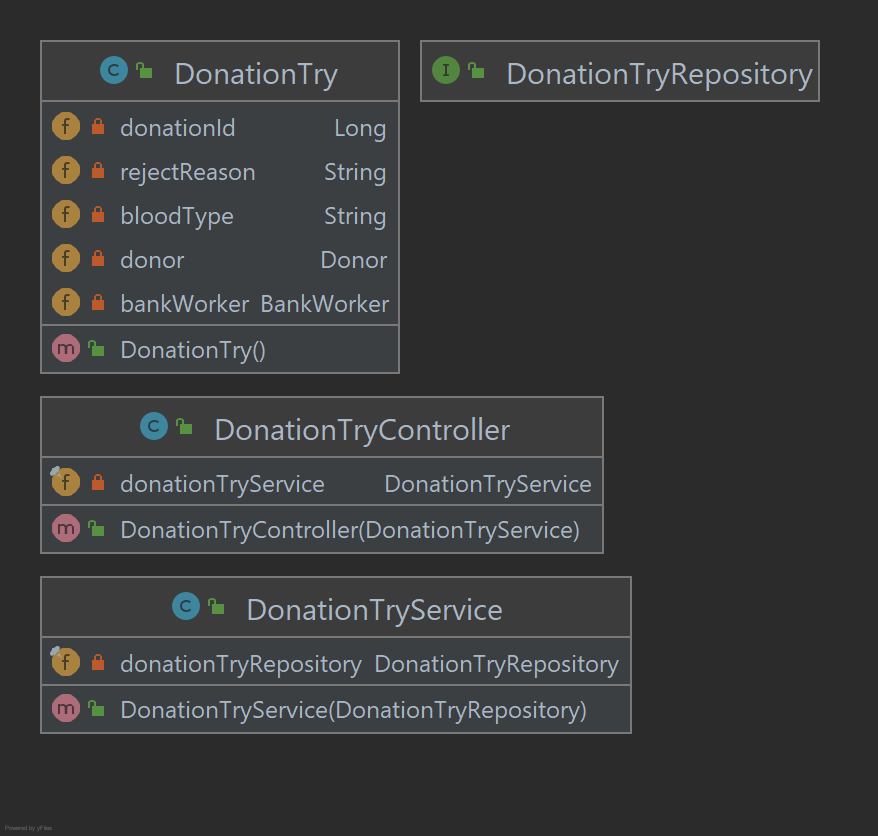
\includegraphics[scale=0.25]{slike/donationtry.png}
        			\centering
        			\caption{Dijagram razreda vezanih za entitet Pokušaj donacije}
        			\label{fig:hztm-stranica}
        		\end{figure}
        		
        		\begin{figure}[H]
                    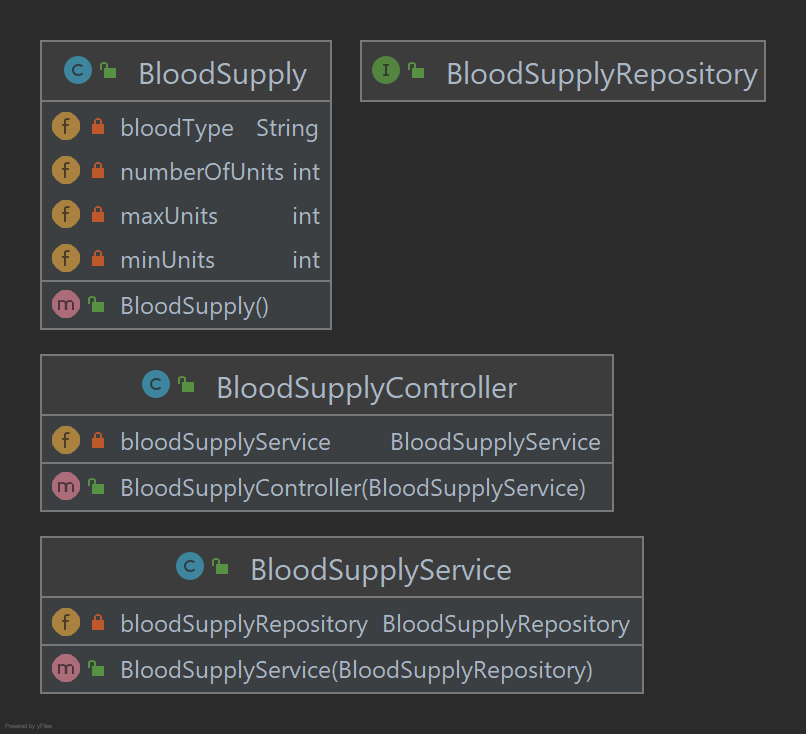
\includegraphics[scale=0.25]{slike/bloodsupply.png}
        			\centering
        			\caption{Dijagram razreda vezanih za entitet Zaliha krvi}
        			\label{fig:hztm-stranica}
        		\end{figure}
        		
        		\begin{figure}[H]
                    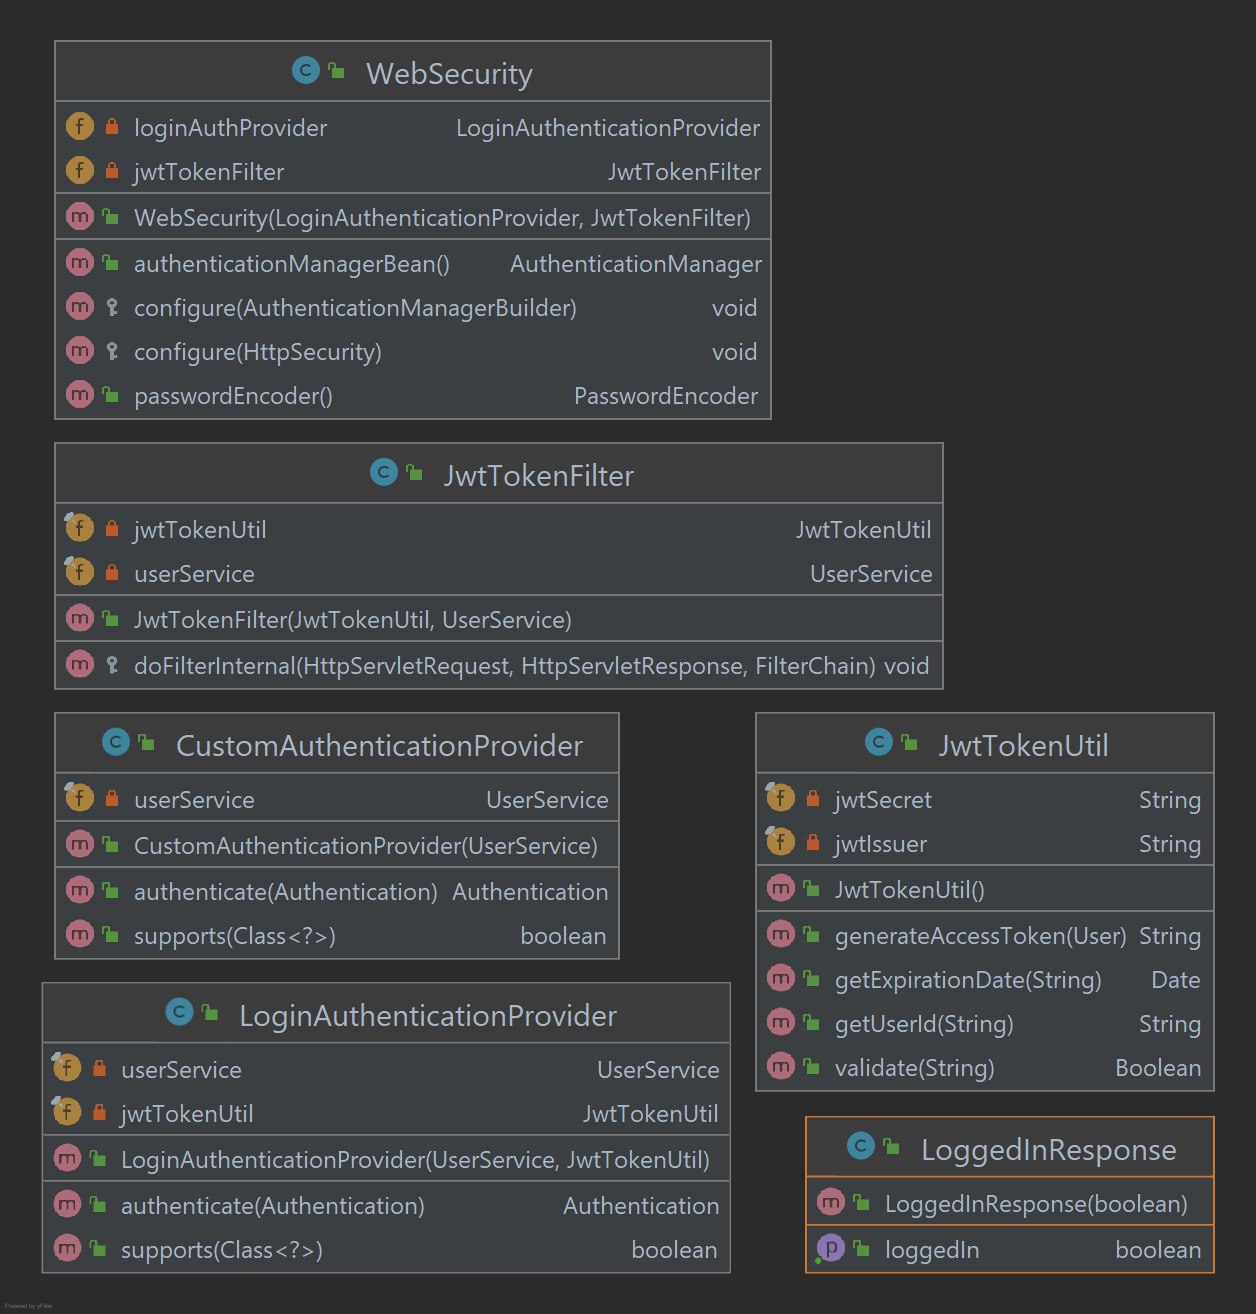
\includegraphics[scale=0.25]{slike/security.png}
        			\centering
        			\caption{Dijagram razreda vezanih za sigurnost i autentikaciju}
        			\label{fig:hztm-stranica}
        		\end{figure}
			
			Zadnja slika sadrži klase vezane za sigurnost i autentikaciju. Radi se o klasama koje pruža Spring. Koriste se Jwt Tokeni (iz biblioteke .jsonwebtoken.jjwt) koji osiguravaju identitet korisnika aplikacije.
			
%			\textbf{\textit{dio 2. revizije}}\\			
			
%			\textit{Prilikom druge predaje projekta dijagram razreda i opisi moraju odgovarati stvarnom stanju implementacije}
			
			
		    
		
		
%		\section{Dijagram stanja}
			
			
%			\textbf{\textit{dio 2. revizije}}\\
			
%			\textit{Potrebno je priložiti dijagram stanja i opisati ga. Dovoljan je jedan dijagram stanja koji prikazuje \textbf{značajan dio funkcionalnosti} sustava. Na primjer, stanja korisničkog sučelja i tijek korištenja neke ključne funkcionalnosti jesu značajan dio sustava, a registracija i prijava nisu. }
			
			

%		\section{Dijagram aktivnosti}
			
%			\textbf{\textit{dio 2. revizije}}\\
			
%			 \textit{Potrebno je priložiti dijagram aktivnosti s pripadajućim opisom. Dijagram aktivnosti treba prikazivati značajan dio sustava.}
			
%			\eject
%		\section{Dijagram komponenti}
		
%			\textbf{\textit{dio 2. revizije}}\\
		
%			 \textit{Potrebno je priložiti dijagram komponenti s pripadajućim opisom. Dijagram komponenti treba prikazivati strukturu cijele aplikacije.}
%	\chapter{Implementacija i korisničko sučelje} \label{implementacija}
		
		
		\section{Korištene tehnologije i alati}
		
% 			\textbf{\textit{dio 2. revizije}}
			 
			 %\textit{Detaljno navesti sve tehnologije i alate koji su primijenjeni pri izradi dokumentacije i aplikacije. Ukratko ih opisati, te navesti njihovo značenje i mjesto primjene. Za svaki navedeni alat i tehnologiju je potrebno \textbf{navesti internet poveznicu} gdje se mogu preuzeti ili više saznati o njima}.
			
        \par{
            Kao platforma za zajednički razvoj projekta, korišten je \href{https://gitlab.com/}{\textcolor{blue}{GitLab}}. Na njoj je dostupan udaljeni repozitorij projekta. Korištenjem GitLaba i \href{https://git-scm.com/}{\textcolor{blue}{Gita}} - sustava za upravljanjem izvornim kodom projekta, članovi razvojnog tima mogu istovremeno raditi na projektu, imajući dostupne promjene čim ih pojedini član tima objavi. Za komunikaciju, razvojni tim koristio je platformu \href{https://slack.com/}{\textcolor{blue}{Slack}}. To je platforma koja omogućava efikasnu komunikaciju članova kroz više specijaliziranih kanala komunikacije.
        }		
        
        \par{
             \href{https://www.jetbrains.com/idea/}{\textcolor{blue}{IntelliJ IDEA}} odabran je kao razvojno okruženje za backend dio aplikacije. JetBrains je razvio to integrirano razvojno okruženje (IDE) koje nudi inteligentnu podršku programiranju u programskom jeziku \href{https://www.java.com/}{\textcolor{blue}{Java}}. 
            
            Kao sredstvo za olakšavanje izrade backend dijela aplikacije korišten je \href{https://spring.io/projects/spring-framework}{\textcolor{blue}{Java Spring Framework}} te
            \href{https://spring.io/projects/spring-boot}{\textcolor{blue}{Spring Boot}}. Spring Framework pojednostavljuje izradu aplikacija koje se izvode na Java virtualnom stroju (engl. \textit{Java Virtual Machine (JVM)}) kroz 4 strategije: 
            \begin{itemize}
                \item  labavo povezivanje objekata ostvareno kroz umetanje ovisnosti (eng. dependency injection) i korištenjem sučelja,
                \item lagan i jednostavan razvoj koristeći obične Java objekte,
                \item deklarativno programiranje kroz aspekte i uobičajene konvencije,
                \item eliminiranje ponavljajućeg koda koristeći aspekte i predloške.
            \end{itemize}
              Spring Boot je aplikacijski okvir koji dodatno proširuje Spring okvir. Njegove glavne značajke su automatska konfiguracija i samostalno odlučivanje o početnim ovisnostima, ovisno o potrebama projekta.
            Kao lokalni spremnik za bazu podataka korišten je            \href{https://www.docker.com/}{\textcolor{blue}{Docker}}. Docker je skup platformi za isporuku softvera u paketima (spremnicima). Popularan je jer olakšava postavljanje lokalnog razvojnog okruženja te njegovo korištenje spremnika omogućava stvaranje više izoliranih okruženja.
            
            \href{https://code.visualstudio.com/}{\textcolor{blue}{VSC}} odabran je kao razvojno okruženje za frontend dio aplikacije. Izvorni kod pisan je u jeziku \href{https://www.javascript.com/}{\textcolor{blue}{JavaScript}} uz upotrebu \href{https://reactjs.org/}{\textcolor{blue}{Reacta}}. React je JavaScript biblioteka koja služi za izgradnju korisničkih sučelja jednostraničnih aplikacija (engl. \textit{Single-page application}). Baziran je na komponentama koje se mogu ponovno koristiti.
            
            Kako bi aplikacija bila javno dostupna, korišten je \href{https://www.heroku.com/}{\textcolor{blue}{Heroku}}. To je platforma za puštanje u pogon te daljnje održavanje aplikacija.
        }

		\par{	
    		Za izradu dokumentacije korišten je \href{https://www.overleaf.com/}{\textcolor{blue}{Overleaf}}, online uređivač dokumenata pisanih u LaTeX markup jeziku. Za izradu dijagrama korišten je \href{https://app.diagrams.net/}{\textcolor{blue}{draw.io}} - online alat za izradu UML, ER te raznih drugih dijagrama.}
	
	    \eject 
	
		\section{Ispitivanje programskog rješenja}
			
			%\textbf{\textit{dio 2. revizije}}\\
			
			 %\textit{U ovom poglavlju je potrebno opisati provedbu ispitivanja implementiranih funkcionalnosti na razini komponenti i na razini cijelog sustava s prikazom odabranih ispitnih slučajeva. Studenti trebaju ispitati temeljnu funkcionalnost i rubne uvjete.}
			
			
			\subsection{Ispitivanje komponenti}
			%\textit{Potrebno je provesti ispitivanje jedinica (engl. unit testing) nad razredima koji implementiraju temeljne funkcionalnosti. Razraditi \textbf{minimalno 6 ispitnih slučajeva} u kojima će se ispitati redovni slučajevi, rubni uvjeti te izazivanje pogreške (engl. exception throwing). Poželjno je stvoriti i ispitni slučaj koji koristi funkcionalnosti koje nisu implementirane. Potrebno je priložiti izvorni kôd svih ispitnih slučajeva te prikaz rezultata izvođenja ispita u razvojnom okruženju (prolaz/pad ispita). }
			
			Ispitivanje je provedeno koristeći Junit biblioteku za Maven. Ispitivani su redovni slučajevi, ali i izazivanje pogrešaka. Testirane su temeljna funkcionalnost aplikacije i funkcije koje upravljaju korisnicima. Slijede priložene slike testova:
			
			    \begin{figure}[H]
                    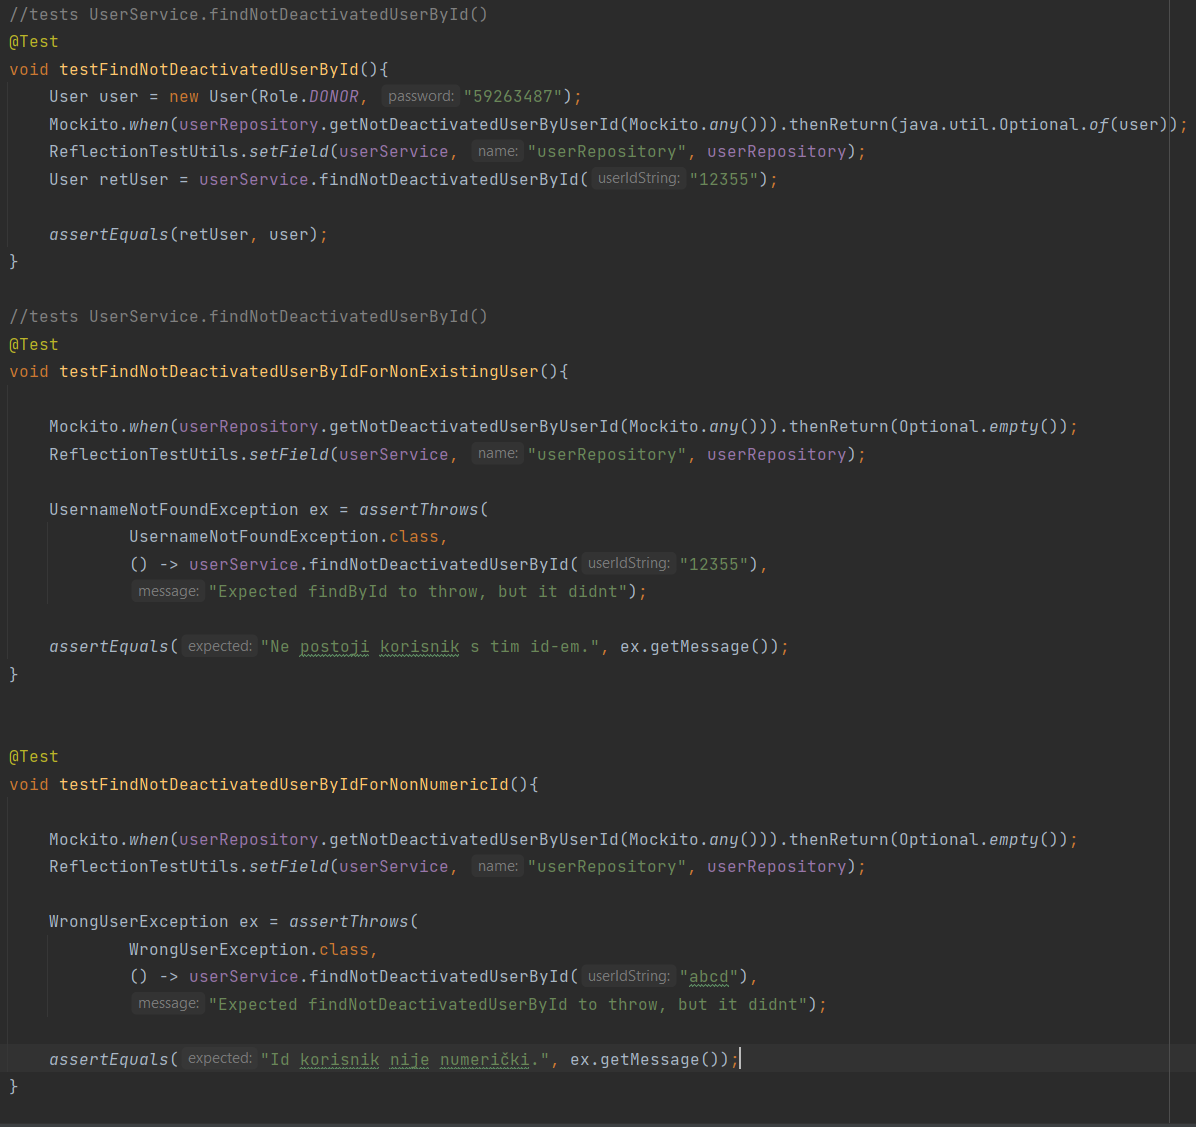
\includegraphics[scale=0.6]{slike/Tests/test1.png}
        			\centering
        			\caption{Testovi, prvi dio}
        			\label{fig:controller}
        		\end{figure}
        		\begin{figure}[H]
                    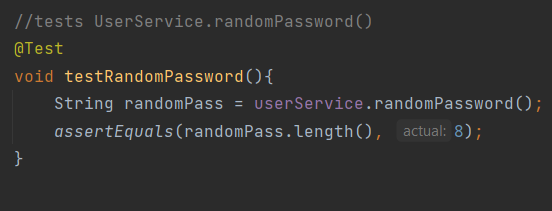
\includegraphics[scale=0.8]{slike/Tests/test2.png}
        			\centering
        			\caption{Testovi, drugi dio}
        			\label{fig:controller}
        		\end{figure}
        		\begin{figure}[H]
                    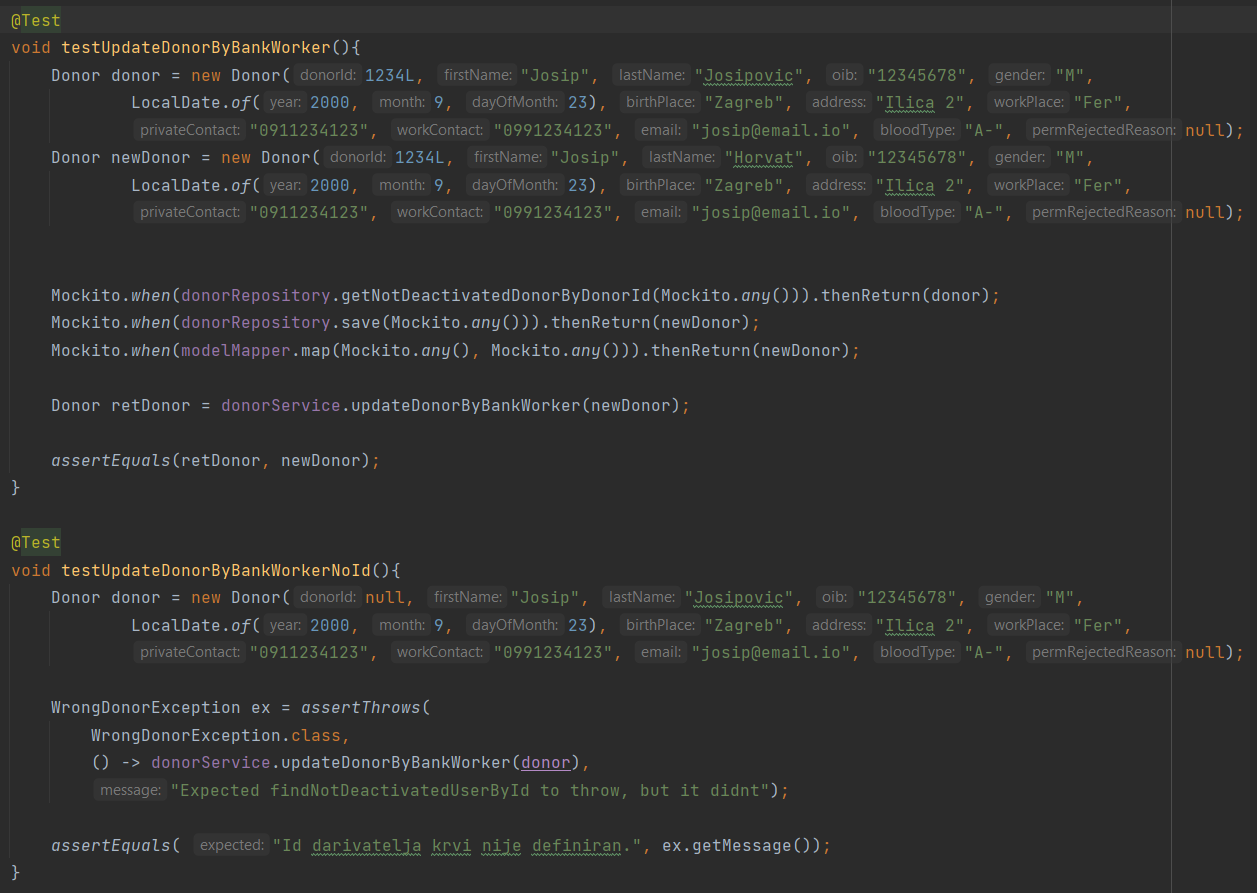
\includegraphics[scale=0.6]{slike/Tests/test3.png}
        			\centering
        			\caption{Testovi, treći dio}
        			\label{fig:controller}
        		\end{figure}
        		\begin{figure}[H]
                    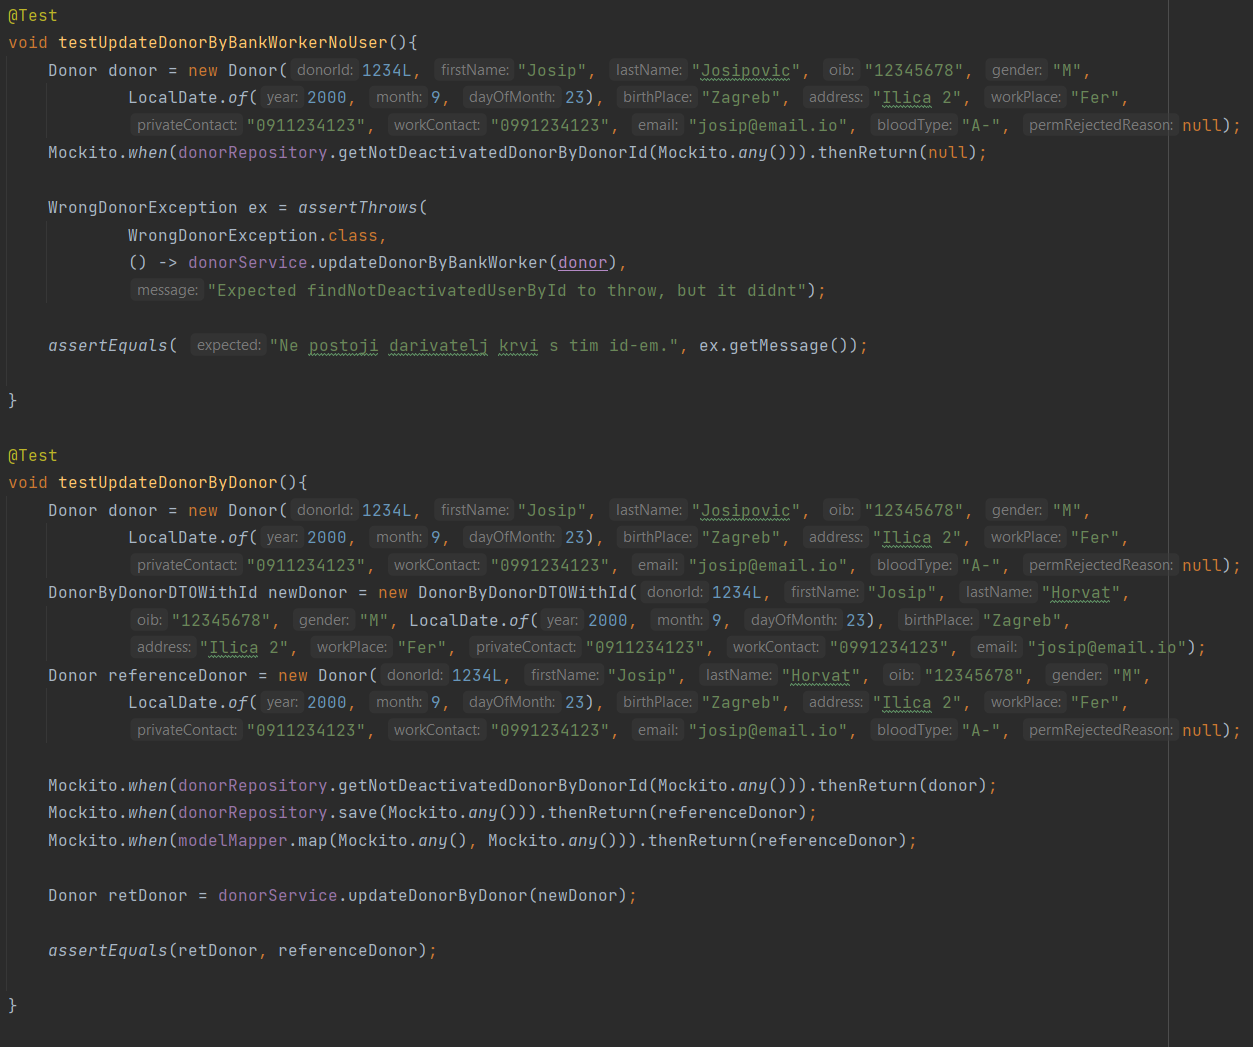
\includegraphics[scale=0.6]{slike/Tests/test4.png}
        			\centering
        			\caption{Testovi, četvrti dio}
        			\label{fig:controller}
        		\end{figure}
        		\begin{figure}[H]
                    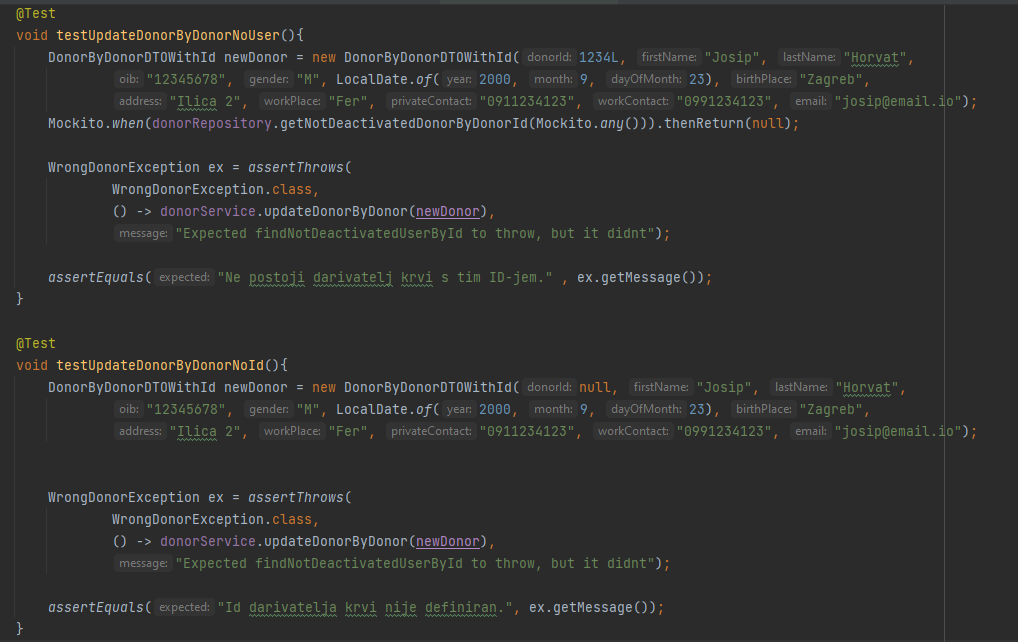
\includegraphics[scale=0.6]{slike/Tests/test5.png}
        			\centering
        			\caption{Testovi, peti dio}
        			\label{fig:controller}
        		\end{figure}
        		
        	%Na veliko zadovoljstvo svih sudionika, s
        	Svi testovi vraćaju prolaz te sve testirane funkcionalnosti rade. Slijedi dokaz:
			
			\begin{figure}[H]
                    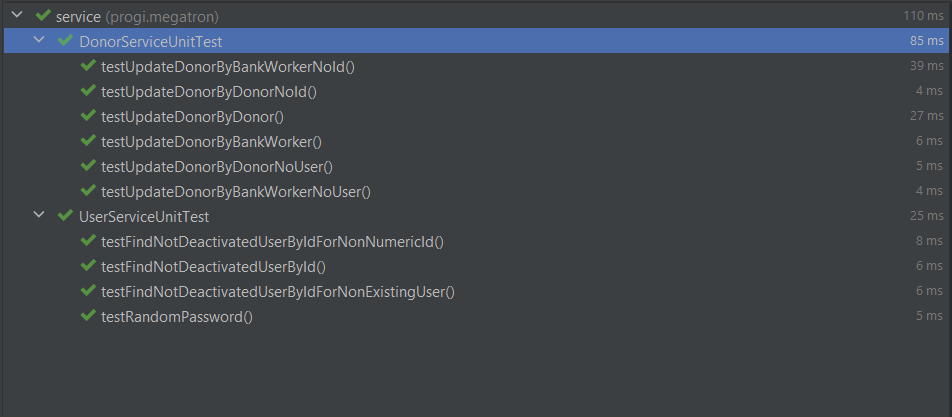
\includegraphics[scale=0.7]{slike/testovi rezultat.png}
        			\centering
        			\caption{Rezultati testiranja}
        			\label{fig:controller}
        		\end{figure}
			
			
			\eject
			\subsection{Ispitivanje sustava}
			
			 %\textit{Potrebno je provesti i opisati ispitivanje sustava koristeći radni okvir Selenium\footnote{\url{https://www.seleniumhq.org/}}. Razraditi \textbf{minimalno 4 ispitna slučaja} u kojima će se ispitati redovni slučajevi, rubni uvjeti te poziv funkcionalnosti koja nije implementirana/izaziva pogrešku kako bi se vidjelo na koji način sustav reagira kada nešto nije u potpunosti ostvareno. Ispitni slučaj se treba sastojati od ulaza (npr. korisničko ime i lozinka), očekivanog izlaza ili rezultata, koraka ispitivanja i dobivenog izlaza ili rezultata.\\ }
			 
			 
			 %\textit{Izradu ispitnih slučajeva pomoću radnog okvira Selenium moguće je provesti pomoću jednog od sljedeća dva alata:}
			 %\begin{itemize}
			 	%\item \textit{dodatak za preglednik \textbf{Selenium IDE} - snimanje korisnikovih akcija radi automatskog ponavljanja ispita	}
			 	%\item \textit{\textbf{Selenium WebDriver} - podrška za pisanje ispita u jezicima Java, C\#, PHP koristeći posebno programsko sučelje.}
			 %\end{itemize}
		 	%\textit{Detalji o korištenju alata Selenium bit će prikazani na posebnom predavanju tijekom semestra.}
			
			Koristeći Selenium IDE plugin za Chrome, provedeno je testiranje sustava. Korištena su četiri testa (slijede njihovi nazivi, opisi te rezultati):
			\begin{itemize}
			    \item 1. \textit{Prijava donora - odjava}:
			    Radi se o jednostavnom testu osnovne funkcionalnosti svakog korisnika. 
			    \begin{figure}[H]
                    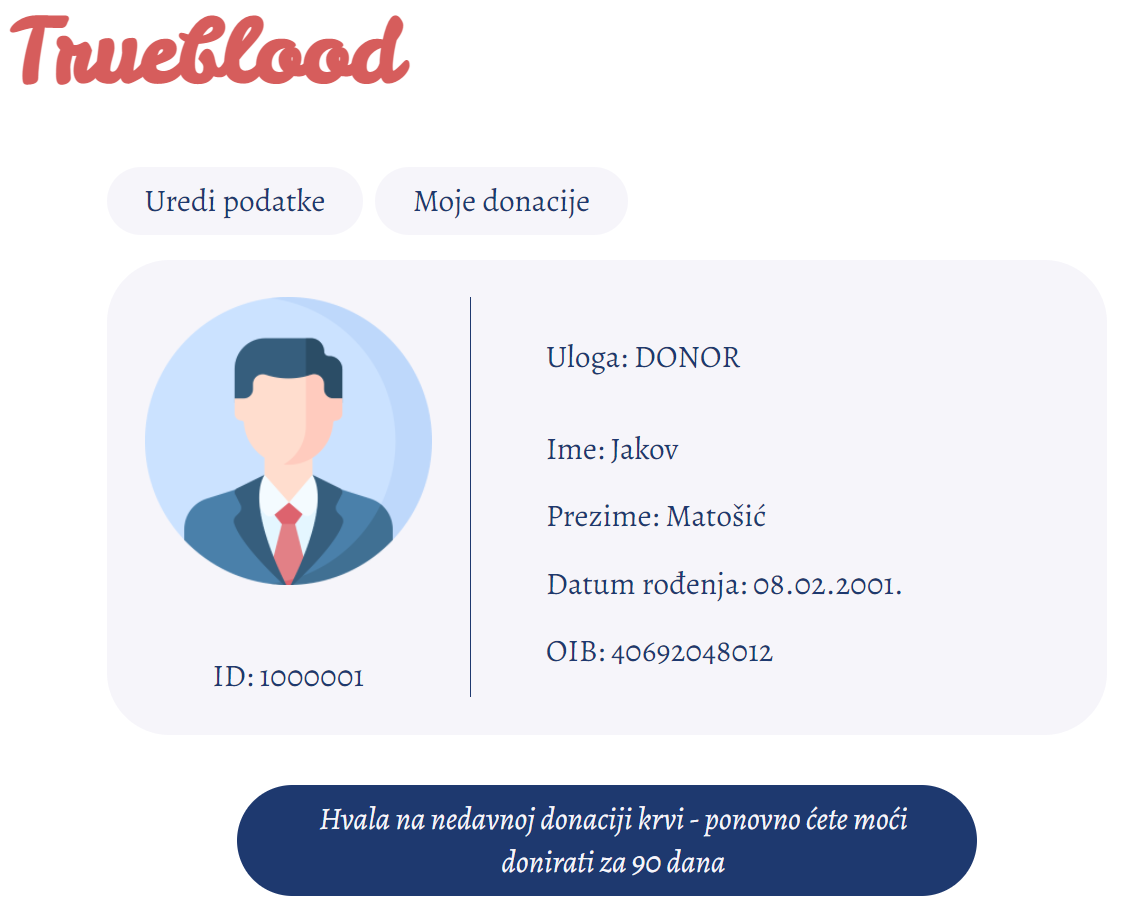
\includegraphics[scale=0.5]{slike/Tests/sistem1.png}
        			\centering
        			\caption{Rezultati prvog testa - profilna stranica prijavljenog korisnika}
        			\label{fig:controller}
        		\end{figure}
			    \item 2. \textit{Registracija (greška: Postojeći OIB)}:
			    Testira javljanje greške pri pravljenju računa sa već zauzetim OIB-om.
			    \begin{figure}[H]
                    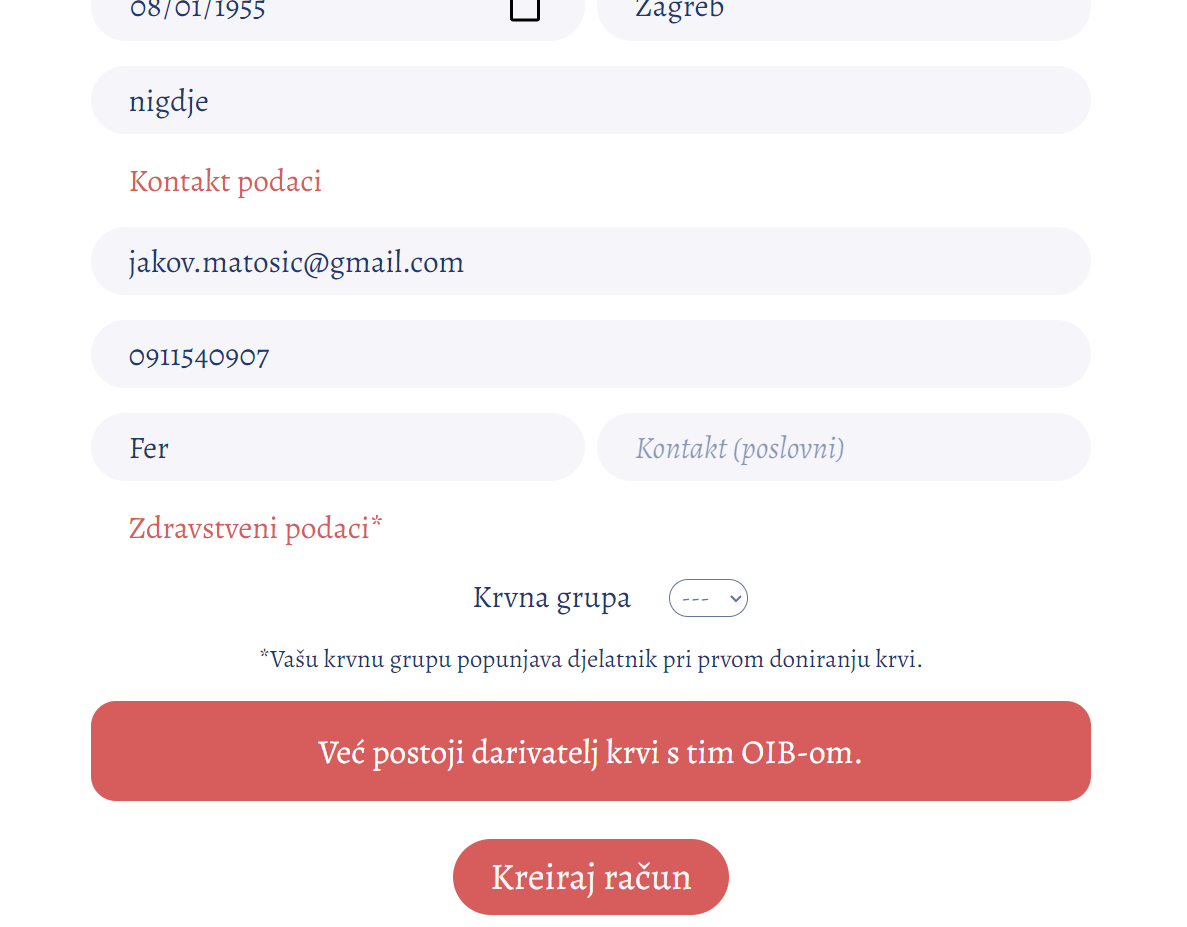
\includegraphics[scale=0.5]{slike/Tests/sistem2.png}
        			\centering
        			\caption{Rezultati drugog testa - greška zbog postojećeg korisnika}
        			\label{fig:controller}
        		\end{figure}
			    \item 3. \textit{prijava radnika - nova donacija (uključuje traženje donora) - odjava}:
			    Testira osnovnu funkcionalnost svakog radnika.
			    \begin{figure}[H]
                    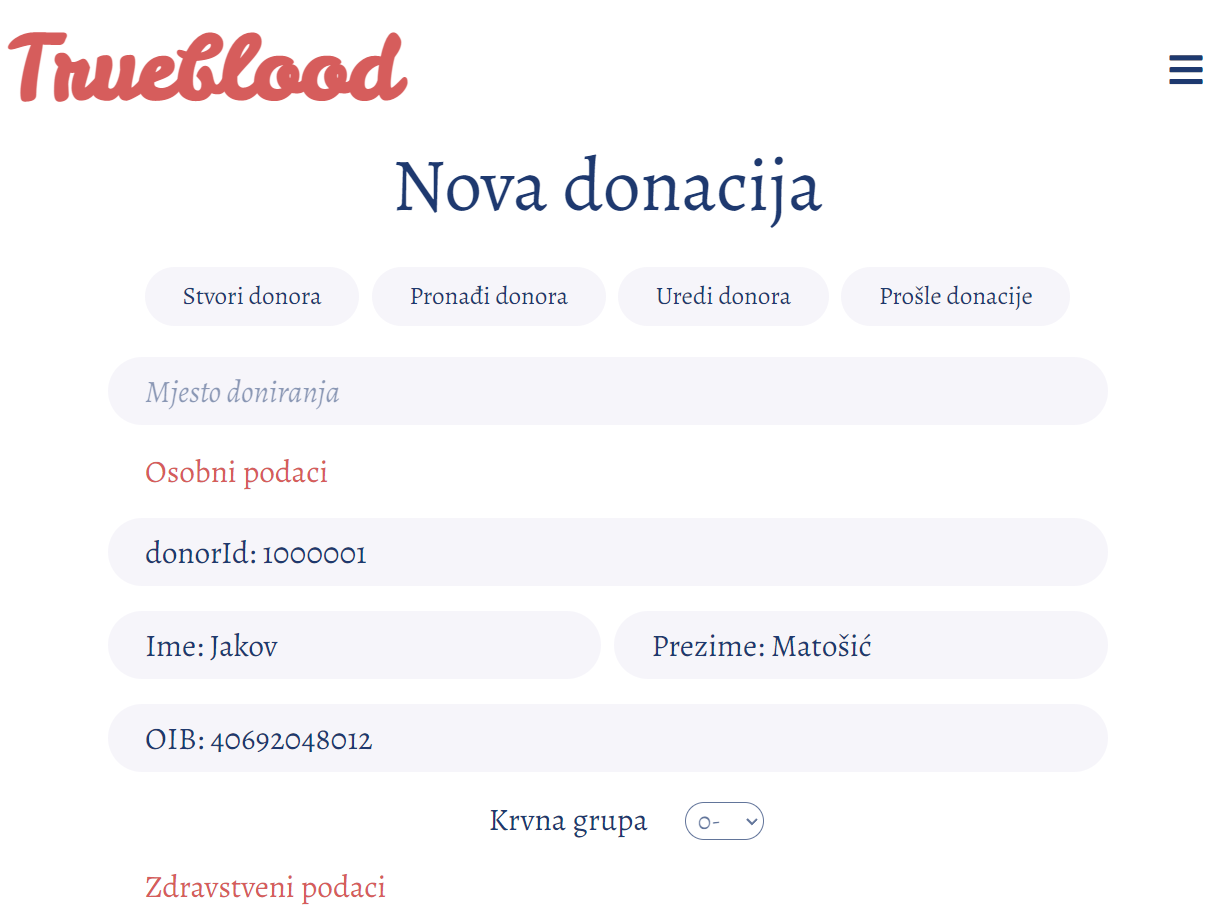
\includegraphics[scale=0.45]{slike/Tests/sistem3.png}
        			\centering
        			\caption{Rezultati trećeg testa - uspješno pronađeni korisnik i započeta donacija}
        			\label{fig:controller}
        		\end{figure}
			    \item 4. \textit{Prijava radnika - registracija novog donora sa greškama (krvna grupa nedefinirana, neispravna adresa e-pošte) - odjava}:
			    \begin{figure}[H]
                    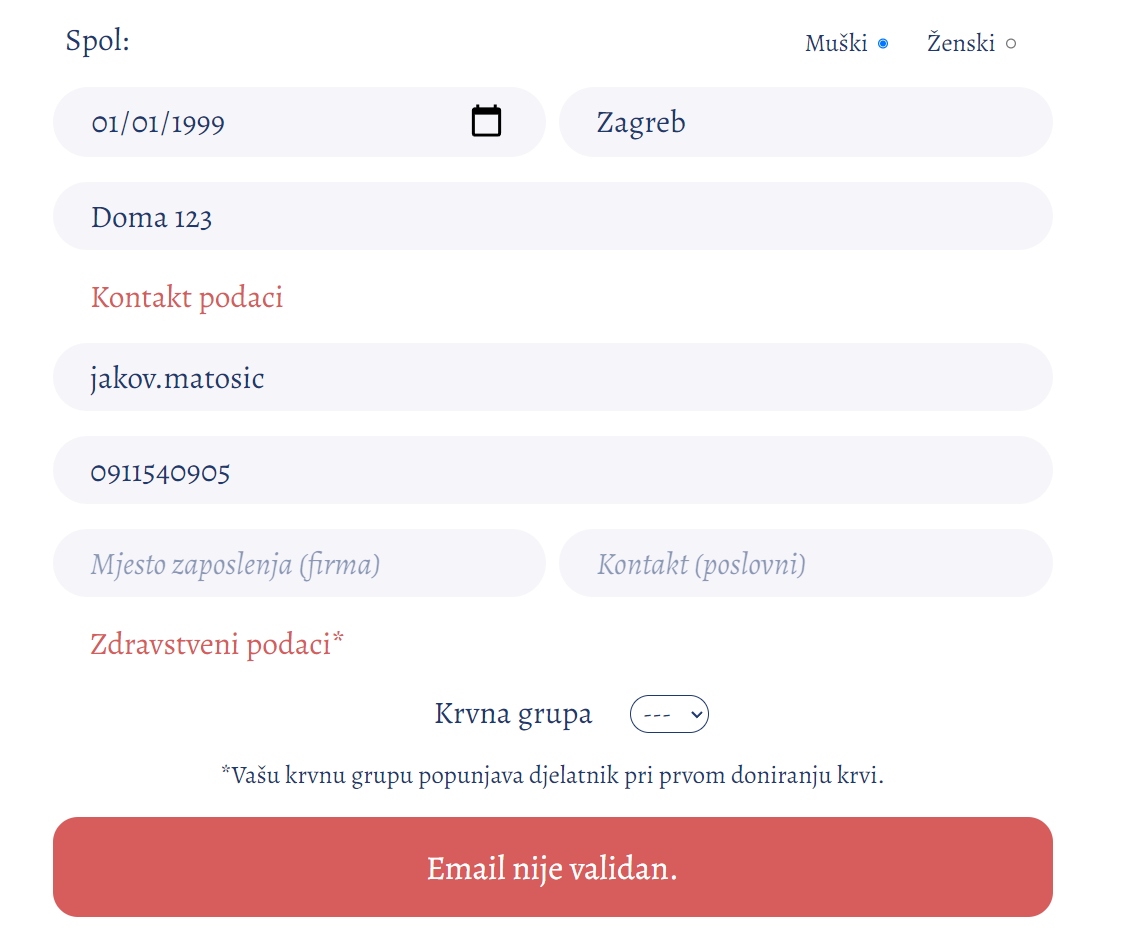
\includegraphics[scale=0.4]{slike/Tests/sistem4.png}
        			\centering
        			\caption{Rezultati četvrtog testa - greška}
        			\label{fig:controller}
        		\end{figure}
        		\begin{figure}[H]
                    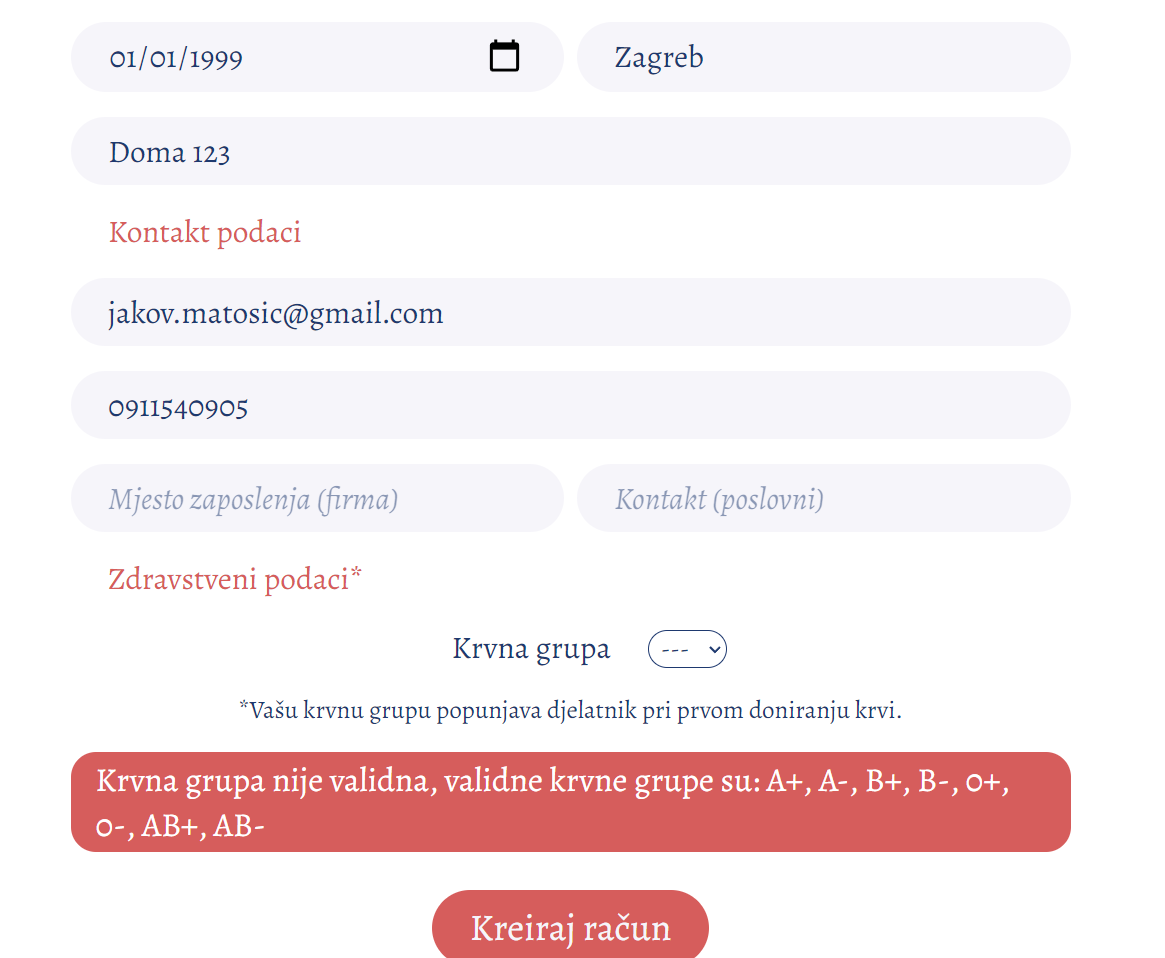
\includegraphics[scale=0.4]{slike/Tests/sistem5.png}
        			\centering
        			\caption{Rezultati četvrtog testa - greška}
        			\label{fig:controller}
        		\end{figure}
			\end{itemize}
			
			
			\eject 
		
		
		\section{Dijagram razmještaja}
			
% 			\textbf{\textit{dio 2. revizije}}
			
			 %\textit{Potrebno je umetnuti \textbf{specifikacijski} dijagram razmještaja i opisati ga. Moguće je umjesto specifikacijskog dijagrama razmještaja umetnuti dijagram razmještaja instanci, pod uvjetom da taj dijagram bolje opisuje neki važniji dio sustava.}
			 
			 \begin{figure}[H]             
    	        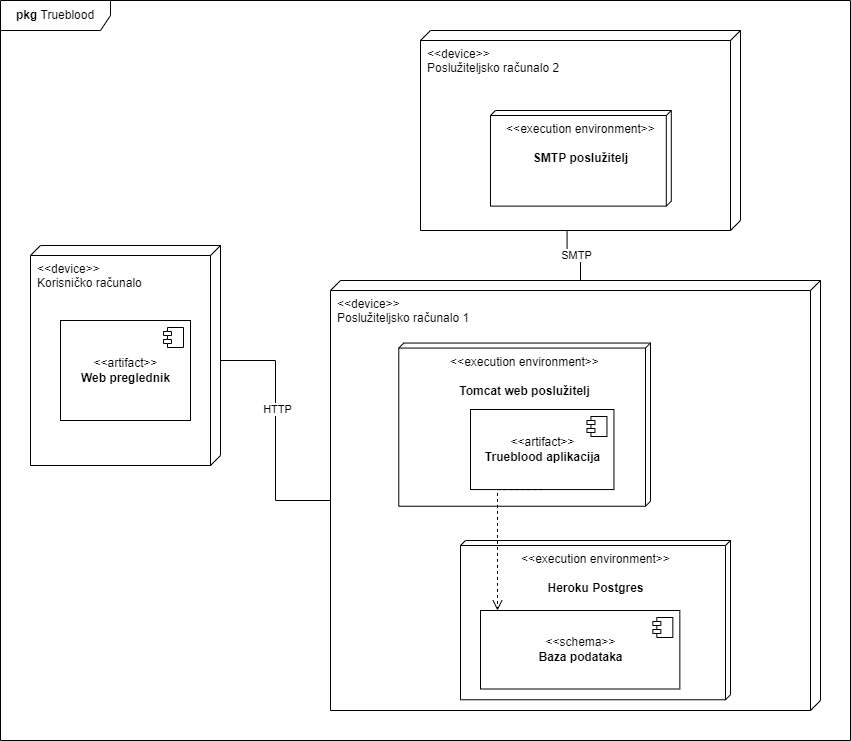
\includegraphics[scale=0.50]{slike/DR1_1.png}
            	\centering
            	\caption{Dijagram razmještaja}
            	\label{fig:dr}
            \end{figure}
            
            \par
            Dijagram razmještaja je UML dijagram koji opisuje topologiju sustava i prikazuje odnos sklopovskih i programskih dijelova. Korisničkom sučelju aplikacije pristupa korisnik sa svog računala putem web preglednika. HTTP vezom dohvaća i šalje podatke na poslužiteljsko računalo na kojem se nalaze web poslužitelj i poslužitelj baze podataka. Web poslužitelj također kontaktira SMTP poslužitelj kako bi se odvila funkcionalnost slanja mailova.
            
			
			\eject 
		
		\section{Upute za puštanje u pogon}
		
% 			\textbf{\textit{dio 2. revizije}}\\
		
			 %\textit{U ovom poglavlju potrebno je dati upute za puštanje u pogon (engl. deployment) ostvarene aplikacije. Na primjer, za web aplikacije, opisati postupak kojim se od izvornog kôda dolazi do potpuno postavljene baze podataka i poslužitelja koji odgovara na upite korisnika. Za mobilnu aplikaciju, postupak kojim se aplikacija izgradi, te postavi na neku od trgovina. Za stolnu (engl. desktop) aplikaciju, postupak kojim se aplikacija instalira na računalo. Ukoliko mobilne i stolne aplikacije komuniciraju s poslužiteljem i/ili bazom podataka, opisati i postupak njihovog postavljanja. Pri izradi uputa preporučuje se \textbf{naglasiti korake instalacije uporabom natuknica} te koristiti što je više moguće \textbf{slike ekrana} (engl. screenshots) kako bi upute bile jasne i jednostavne za slijediti.}
			
			
			 %\textit{Dovršenu aplikaciju potrebno je pokrenuti na javno dostupnom poslužitelju. Studentima se preporuča korištenje neke od sljedećih besplatnih usluga: \href{https://aws.amazon.com/}{Amazon AWS}, \href{https://azure.microsoft.com/en-us/}{Microsoft Azure} ili \href{https://www.heroku.com/}{Heroku}. Mobilne aplikacije trebaju biti objavljene na F-Droid, Google Play ili Amazon App trgovini.}
			
			\textbf{Instalacija i pokretanje Docker servisa}
			\begin{itemize}
    		    \item \text{Preuzmite prikladnu verziju \href{https://hub.docker.com/editions/community/docker-ce-desktop-windows/}{\textcolor{blue}{Dockera}} za svoj operacijski sustav}
			    \item Pokrenite Docker servis
			    
            	    \begin{minipage}{\linewidth}             
    	    	        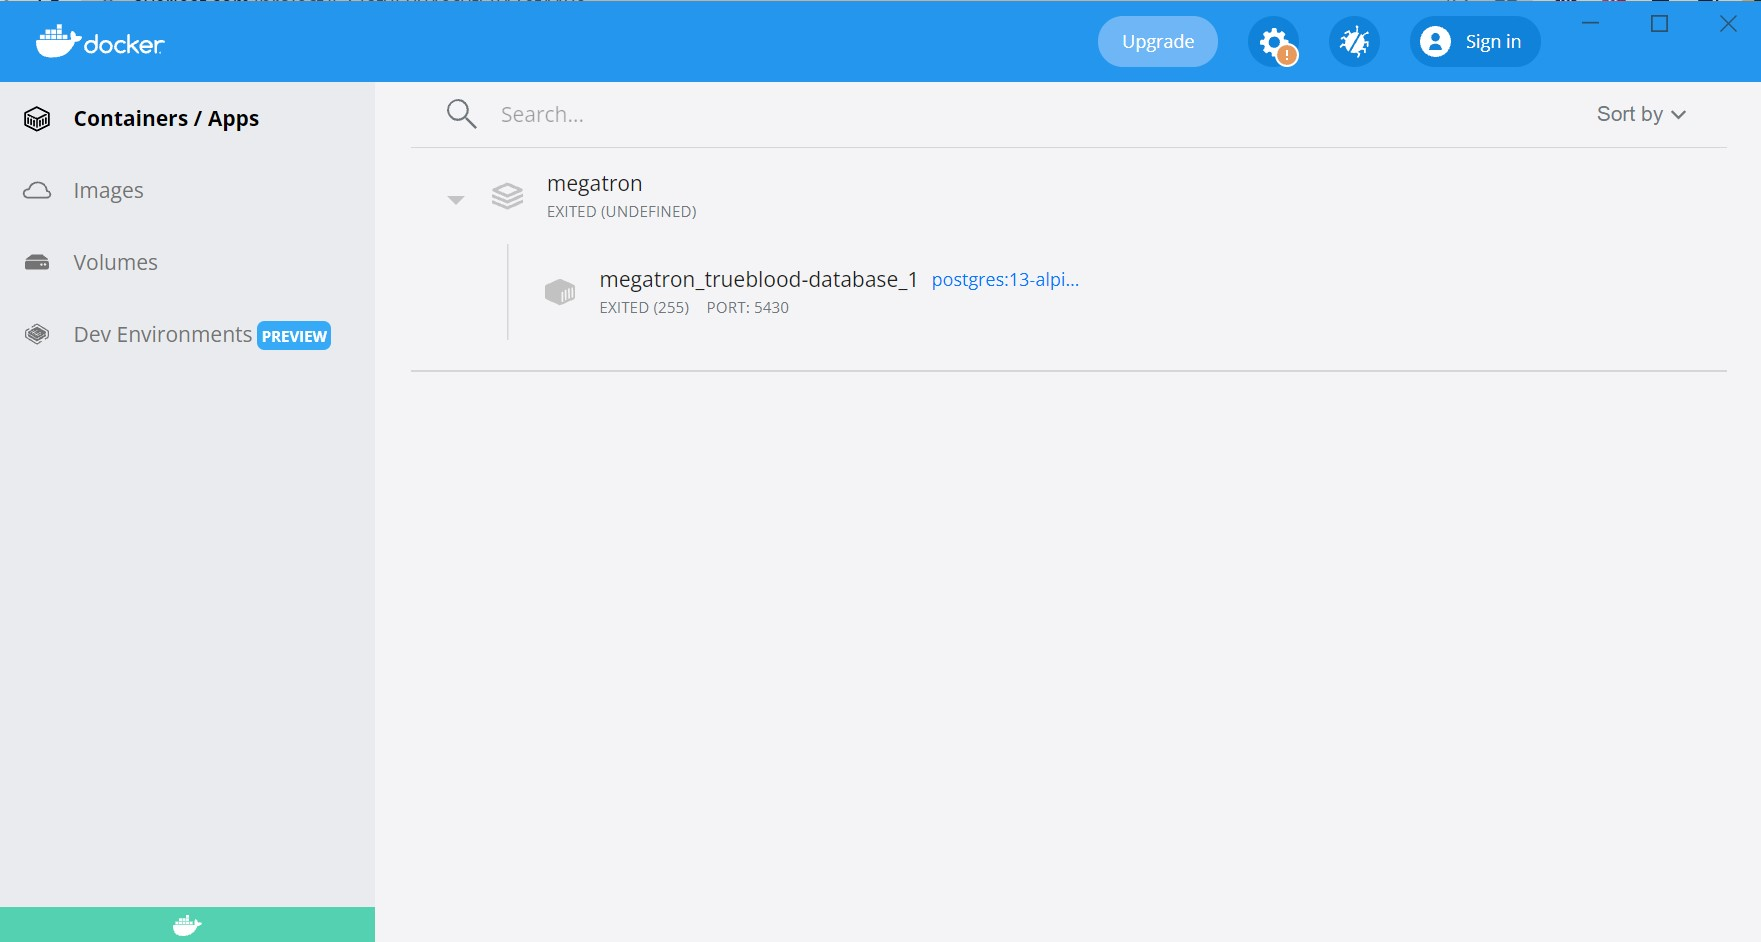
\includegraphics[scale=0.45]{slike/deploy/Docker1.jpg}
                    	\centering
                    	\captionof{figure}{Korisničko sučelje Dockera}
                    	\label{fig:DockerUI}
                    \end{minipage}
    	    	
    	    	\item U terminalu pozicioniranom u korijenskom direktoriju projekta upišite naredbu 

        	    	\begin{verbatim}
        $ docker-compose up
        	    	\end{verbatim}
        	    	
            	    \begin{minipage}{\linewidth}
                        \centering
                    	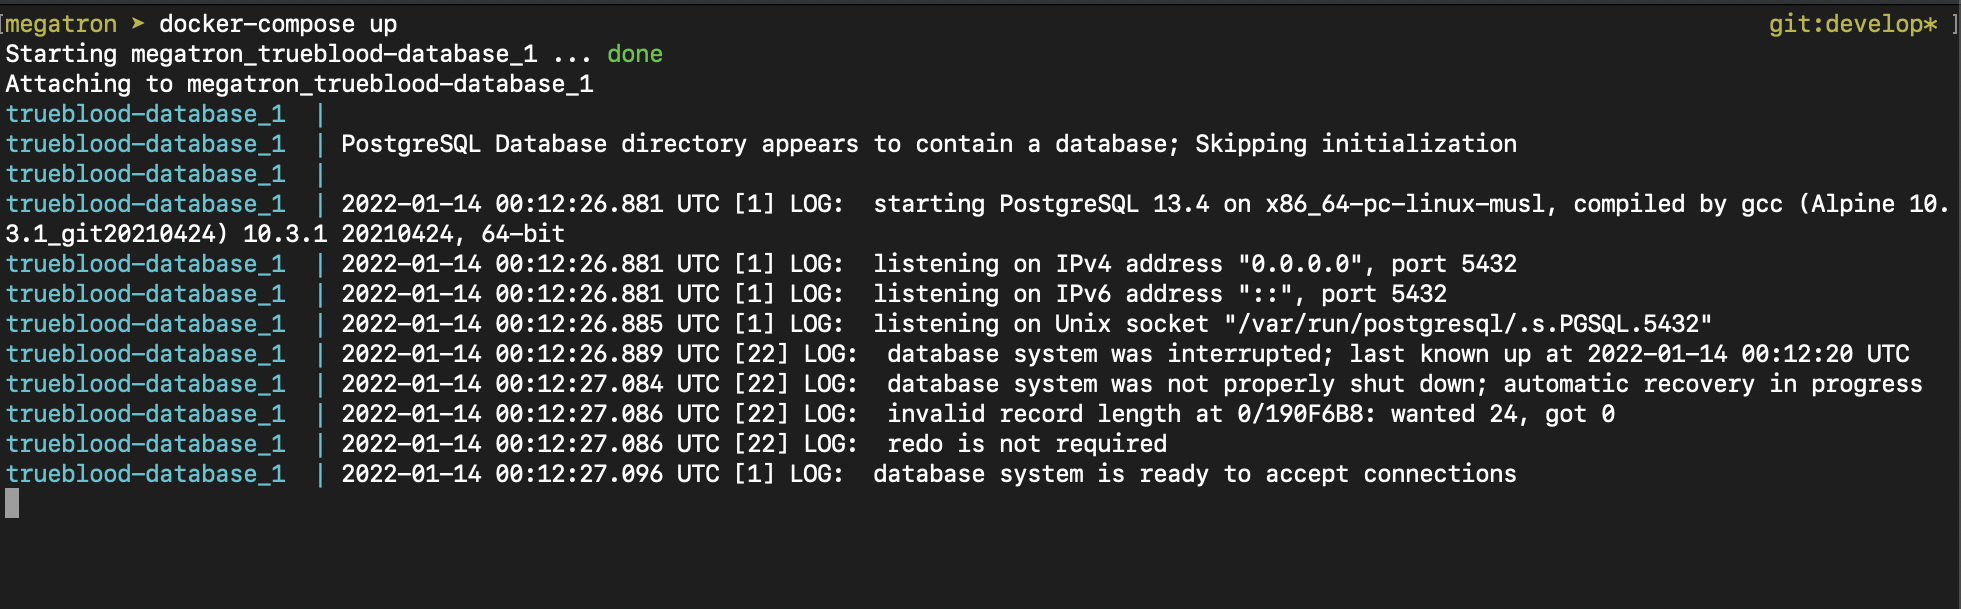
\includegraphics[scale=0.4]{slike/deploy/Docker2.png} %veličina slike u
                        \captionof{figure}{Pokretanje Docker spremnika}
                    \end{minipage}
        	    	%\begin{figure}
                    %	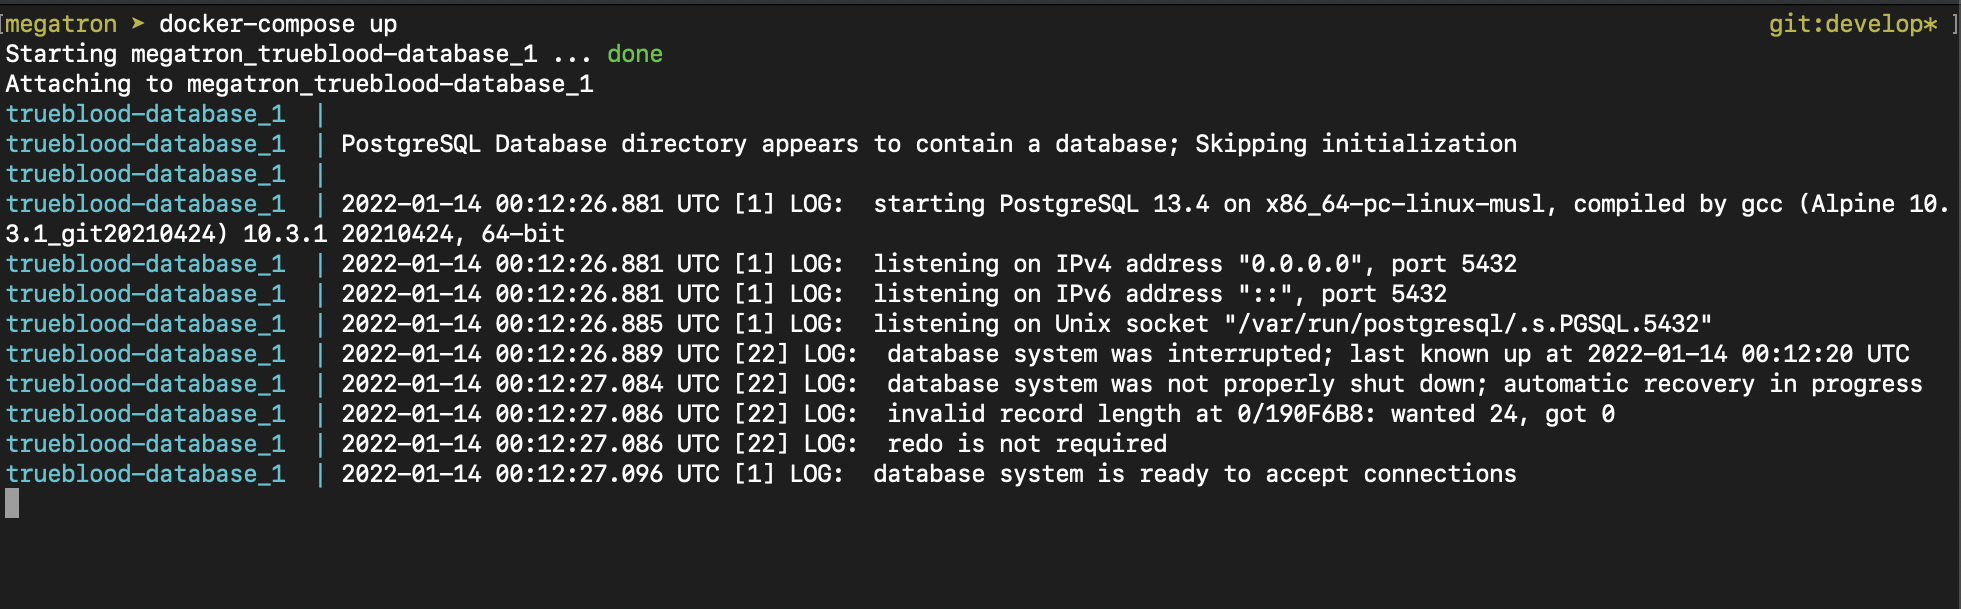
\includegraphics[scale=0.4]{slike/deploy/Docker2.png} %veličina slike u odnosu na originalnu datoteku i pozicija slike
            		%	\centering
            		%	\caption{Pokretanje Docker spremnika}
        		
        	    	%end{figure}
        	    
        	    \item Otvorite drugi terminal te u korijenskom direktoriju projekta upišite naredbu
        	    
            	    \begin{verbatim}
        $ psql -h localhost -p 5430 -d Trueblood -U admin
            	    \end{verbatim}
			    i password "admin"
			        
            	    \begin{minipage}{\linewidth}
                    	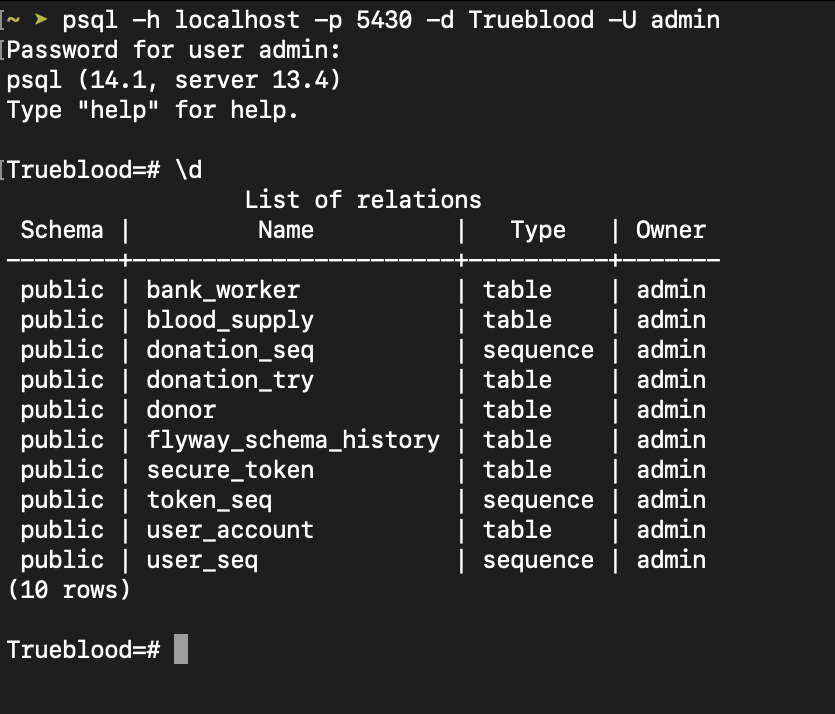
\includegraphics[scale=0.8]{slike/deploy/psql-primjer.png} %veličina slike u odnosu na originalnu datoteku i pozicija slike
            			\centering
            			\captionof{figure}{Spajanje na bazu pomoću alata PSQL}
        		        \label{fig:psql}
                    \end{minipage}
			    
			\end{itemize}
			\eject
			
			\textbf{Postavljanje frontenda}
			    \begin{itemize}
			        \item Preuzmite i instalirajte Node.js i			         \href{https://docs.npmjs.com/downloading-and-installing-node-js-and-npm}{\textcolor{blue}{npm}}
			        
			        \item Preuzmite yarn narebom 
			        \begin{verbatim}
			            $ npm install --global yarn
			        \end{verbatim}
			        
			        \item Pokretanjem naredbe
			        \begin{verbatim}
			            $ yarn install
			        \end{verbatim}
			        instalirat će se potrebni paketi
			        
			        \item Razvojni poslužitelj (engl. \textit{development server}) pokreće se naredbom 
			        \begin{verbatim}
			            $ yarn start
			        \end{verbatim}
			        
            	    \begin{minipage}{\linewidth}
                    	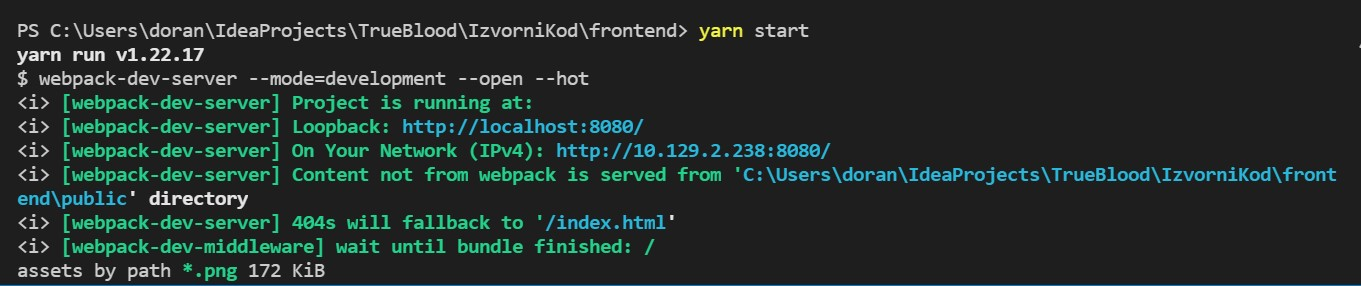
\includegraphics[scale=0.6]{slike/deploy/yarn-start.jpg} %veličina slike u odnosu na originalnu datoteku i pozicija slike
            			\centering
            			\captionof{figure}{Pokretanje razvojnog poslužitelja}
        		        \label{fig:yarnstart}
                    \end{minipage}
			        
			    \end{itemize}
			\eject
			    
			\textbf{Javno puštanje aplikacije u pogon}
    			\begin{itemize}
    			    \item Napravite \href{https://signup.heroku.com/}{\textcolor{blue}{Heroku korisnički račun}}
    			    \item Instalirajte \href{https://devcenter.heroku.com/articles/heroku-cli}{\textcolor{blue}{Heroku CLI}}
    			    \item Koristeći naredbu 
    			    \begin{verbatim}
    			        $ heroku login
    			    \end{verbatim}
    			    pokrenite postupak autorizacije
			    \end{itemize}
    			 %\eject
    			 \textbf{Primjeri korištenja Heroku alata} \newline
    			 \textit{Navedeni primjeri mogu se koristiti i s trueblood-fe}
    			 \begin{itemize}
    			 \item Za ponovno pokretanje aplikacije upišite naredbu
    			 \begin{verbatim}
    			     $ heroku restart --app trueblood-be
    			 \end{verbatim}
    			 \item Za uvid u zapisnik aplikacije
    			 \begin{verbatim}
    			    $ heroku logs --tail --app trueblood-be
    			 \end{verbatim}

                \item Pregled trenutnih build radnji
                \begin{verbatim}
        $ heroku builds --app trueblood-be
                \end{verbatim}
                
                \item Povezivanje s bazom pokreće se naredbom
                \begin{verbatim}
        $ heroku pg:psql --app trueblood-be
                \end{verbatim}
                \textit{ova naredba nije dostupna za trueblood-fe}
    			\end{itemize}
    		Status cjevovoda moguće je provjeriti na GitLabu. U slučaju podbacivanja cjevovoda te dobivanja poruke \textit{Your account has reached its concurrent builds limit} u zapisniku aplikacije, potrebno je ponovno pokrenuti aplikaciju.
			\eject 
%	\chapter{Zaključak i budući rad}
		
		\textbf{\textit{dio 2. revizije}}\\
		
		 \textit{U ovom poglavlju potrebno je napisati osvrt na vrijeme izrade projektnog zadatka, koji su tehnički izazovi prepoznati, jesu li riješeni ili kako bi mogli biti riješeni, koja su znanja stečena pri izradi projekta, koja bi znanja bila posebno potrebna za brže i kvalitetnije ostvarenje projekta i koje bi bile perspektive za nastavak rada u projektnoj grupi.}
		
		 \textit{Potrebno je točno popisati funkcionalnosti koje nisu implementirane u ostvarenoj aplikaciji.}
		
		\eject 
	\chapter*{Popis literature}
		\addcontentsline{toc}{chapter}{Popis literature}
	 	
% 		\textbf{\textit{Kontinuirano osvježavanje}}
	
%		\textit{Popisati sve reference i literaturu koja je pomogla pri ostvarivanju projekta.}
		
		
		\begin{enumerate}
			
			
			\item  Programsko inženjerstvo, FER ZEMRIS, \url{http://www.fer.hr/predmet/proinz}
			
			\item  I. Sommerville, "Software engineering", 8th ed, Addison Wesley, 2007.
			
			\item  T.C.Lethbridge, R.Langaniere, "Object-Oriented Software Engineering", 2nd ed. McGraw-Hill, 2005.
			
			\item  I. Marsic, Software engineering book``, Department of Electrical and Computer Engineering, Rutgers University, \url{http://www.ece.rutgers.edu/~marsic/books/SE}
			
			\item  The Unified Modeling Language, \url{https://www.uml-diagrams.org/}
			
			\item  Astah Community, \url{http://astah.net/editions/uml-new}
			
			\item  https://www.techopedia.com/definition/24649/three-tier-architecture
			
			\item https://www.w3.org/TR/wsdl.html
			\item https://reactjs.org/
			\item https://spring.io/projects/spring-boot
		\end{enumerate}
		
		 
	
	
	\begingroup
	\renewcommand*\listfigurename{Indeks slika i dijagrama}
	\renewcommand*\listtablename{Indeks tablica}
	\let\clearpage\relax
	\listoffigures
	\vspace{10mm}
	\listoftables
	\endgroup
	\addcontentsline{toc}{chapter}{Indeks slika i dijagrama}


	
	\eject 
		
	\chapter*{Dodatak: Prikaz aktivnosti grupe}
		\addcontentsline{toc}{chapter}{Dodatak: Prikaz aktivnosti grupe}
		
		\section*{Dnevnik sastajanja}
		
%		\textbf{\textit{Kontinuirano osvježavanje}}\\
		
%		 \textit{U ovom dijelu potrebno je redovito osvježavati dnevnik sastajanja prema predlošku.}
		
		\newcommand{\mylabel}[2]{#2\def\@currentlabel{#2}\label{#1}}  % za napraviti labele poput 4.1
		
		\begin{packed_enum}
			\item  sastanak
			
			\item[] \begin{packed_item}
				\item Datum: 5. listopada 2021.
				\item Prisustvovali: Svi
				\item Teme sastanka:
				\begin{packed_item}
                    \item Uspostava svih članova tima
                \end{packed_item}
			\end{packed_item}
			
			\bigskip
			\item  sastanak
			\item[] \begin{packed_item}
				\item Datum: 17. listopada 2021.
				\item Prisustvovali: Svi
				\item Uspostava GitLab repozitorija
				\item Uspostava SSH ključeva
				\item Uspostavljena platforma za komunikaciju (Slack)
				\item Prva okvirna podjela poslova:
				\item[] \begin{packed_item}
					\item Ana - backend (Spring)
		            \item Vukota - backend (Spring)
		            \item Jakov - backend, testovi
		            \item Dora - backend
		            \item Marko - full-stack
		            \item Toni - full-stack, organizacija
		            \item Borna - frontend (UI)
				\end{packed_item}
				
		    	\item Zadatak za prvi tjedan:
		    	\item[] \begin{packed_item}
		            \item Do četvrtka:
                	\begin{packed_item}
	                    \item Upoznati se sa radnom okolinom, gitom, softverom koji se koristi
	                    \item Pročitati zadatak s razumijevanjem
	                    \item Zabilježiti sva pitanja koja se pojave	
	                \end{packed_item}
                    \item Četvrtak:
                    \item[] \begin{packed_item}
	                    \item Sastanak s asistentima (labos) u 11:00
	                    \item Sastanak u 13:00
	                \end{packed_item}      
                \end{packed_item}
			\end{packed_item}
			
			\bigskip
			\item sastanak
			\item[] \begin{packed_item}
				\item Datum: 21. listopada 2021.
		        \item Sastanak s asistentom i demosom: odgovorili na pitanja
		        \item[] \begin{packed_item}
    		        \item Prisutni: Toni, Ana, Jakov, Marko
    		        \item u aplikaciji napraviti formular s pitanjima. (sve su da ne pitanja, nema opisivanja)
    		        \item 1 tablica sa svim userima u sustavu - ime prezime username pass mail role id(općeniti)
    		        \item aktivacijski mail ako na doniranju kreira račun
    		        \item *pazi ima jos jedan nacin pada
    		        \item DonorId je primarni ključ, a OIB alternativni ključ
		        \end{packed_item}
		        
		        \item Sastanak grupni:
		        \item[] \begin{packed_item}
		            \item Prisutni: Ana, Vukota, Jakov, Toni, Marko, Dora
		            \item crtanje UC dijagrama
		            \item backend brainstorming oko funkcionalnosti
		            \item userId=donorId
		            \item za account postoje 2 bool varijable 1) account inicijalno aktiviran (pokreće se otvaranjem linka u mailu) i 2) account trajno deaktiviran (od strane admina) 
	            \end{packed_item}
	            
	            \item Zadatci do idućeg sastanka:
	            \item[] \begin{packed_item}
	               \item Ana - radi bazu (edrplus)
	               \item Marko - poboljšati organizaciju gita, inicijalizacija direktorija za kod
	               \item Dora - UC dijagrami, sekvencijski dijagrami
	               \item Toni - UC dijagrami, sekvencijski dijagrami
	               \item Vukota - postavljanje LaTeX-a i inicijalizacija projektne dokumentacije
	               \item Jakov - Uvođenje u Spring
	               \item Borna - Uvođenje u React
	            \end{packed_item}
	            \item Idući sastanak: Četvrtak(28.10.) - sastanak sa asistentima i grupni sastanak (11h, 13h)
	        \end{packed_item}
	        
	        \bigskip  % ili \vspace{\baselineskip} - otprilike isti
	        \item sastanak
            \item[] \begin{packed_item}
               \item Datum: 28. listopada 2021.
               \item Sastanak s asistentom i demosom: odgovori na pitanja, demonstracija inicijalnih UC, demonstracija dizajna stranice
               \item[] \begin{packed_item}
                    \item Prisustvovali: Toni, Ana, Dora, Borna, Jakov, Luka
                    \item odgovorena pitanja iz maila
                    \item prokomentirani UC dijagrami --> treba reducirati
                    \item predstavljen model baze podataka, spomenute nove mogućnosti platforme
                    \item predstavljen idejni dizajn frontenda
                    \item predloženi alati Overleaf (Latex), Dbdiagram.io, Hibernate
               \end{packed_item}
               \item Sastanak grupni:
               \item[] \begin{packed_item}
                    \item Prisustvovali: svi
                    \item dogovor oko daljnjeg frontend dizajna
                    \item dogovoren sastanak backend podtima (subota) radi inicijalizacije dockera
               \end{packed_item}
               \item Zadatci do idućeg sastanka:
               \item[] \begin{packed_item}
                    \item Toni - Popravak i nadogradnja UC dijagrama i crtanje sekvencijskih; inicijalizacija dokumentacije
                    \item Dora, Jakov - Upoznavanje sa Springom
                    \item Ana - dorada baze podataka, istražiti opcije predstavljene na sastanku; docker
                    \item Vukota - docker, pisanje inicijalnog readme.md
                    \item Borna - nastavak idejnih dizajna stranice, inicijalna konstrukcija frontend dijela stranice
                    \item Marko - održavanje gita, rad s Bornom na frontendu
               \end{packed_item}
               \item Idući sastanak: Backend - subota(30.10.), ostali - četvrtak (4.11.)
            \end{packed_item}
            
            \bigskip
            \begin{enumerate}
            \noindent \item[\mylabel{itm41}{4.1.}]  sastanak (backend)
            \item[] \begin{packed_item}
                \item Datum: 30. listopada 2021.
                \item Prisustvovali: Ana, Luka, Jakov, Dora
                \item uspostava Dockera (baza)
                \item početak rada na useru (Ana)
                \item početak rada na bloodSupplyju (Dora i Jakov)
                \item pomaganje (Luka)
                \item Idući sastanak: svi - četvrtak (4.11.)
            \end{packed_item}
            \end{enumerate}
            
            \bigskip
            \item sastanak
            \item[] \begin{packed_item}
                \item Datum: 4. studenog 2021.
                \item Sastanak s asistentima:
                \item[] \begin{packed_item}
                    \item Prisustvovali: Toni, Ana, Dora, Borna, Jakov, Vukota
                    \item maknuti field brojDonacija iz donora
                    \item maknuti NOT NULL sa bloodType
                    \item glavni sudionik ne pisati pod sudionici u opisima UC-jeva
                    \item UC dodavanje računa moguće razdvojiti na tri (da imamo u svakom po jednog glavnog sudionika)
                    \item za generičku funkcionalnost treba pokazati da imamo session, držimo session, i možemo kreirati usera (U tablici 3 prikazano što treba)
                \end{packed_item}
                \item Grupni sastanak:
                \item[] \begin{packed_item}
                    \item Prisustvovali: Svi
                    \item edukacija o gitu
                    \item dogovor da idući tjedan bude gotov login page i registracija
                    \item oformljen zajednički account za uređivanje dokumentacije
                    \item pri stvaranju accounta, na mail se šalje link za aktivaciju I RANDOM LOZINKA, a postojat će opcija "Promijeni lozinku"
                    \item za generičku funkcionalnost, lozinka se ispisuje u terminal
                \end{packed_item}
                \item Zadatci za idući tjedan:
                \item[] \begin{packed_item}
                    \item Vukota: završi sve modele (klase kao relacije u bazi)
                    \item Ana: Endpoint (create user)
                    \item Dora: Endpoint (create donor)
                    \item Jakov: Istražiti Heroku (deploy aplikacije), Testovi (backend)
                    \item Borna: Dovršiti login page (popravci) i dizajn za stranicu registracije
                    \item Marko: spajanje frontenda i backenda
                    \item Toni: Popravak UC dijagrama, pisanje dokumentacije
                \end{packed_item}
            \end{packed_item}
            
            \bigskip
            \item sastanak
            \item[] \begin{packed_item}
                \item Datum: 10. studenog 2021.
                \item Prisustvovali: svi
            	\item rad na web securityju
            	\item brainstorm o mergeu frontenda i backenda kao priprema za deploy
            	\item podjela posla oko dokumentacije
            	\item Zadatci za dalje:
            	\item[] \begin{packed_item}
            	   \item Borna: Napisati ukratko dio vezan za frontend u dokumentaciju - arhitektura sustava
		            \item Marko, Ana, Vukota: Web security (omogućiti funkcionalnost logina)
		            \item Toni, Jakov: Rad na dokumentaciji
            	\end{packed_item}
            \end{packed_item}
            
            \bigskip
            \noindent \item[\mylabel{itm61}{6.1.}]  sastanak
            \item[] \begin{packed_item}
                \item Datum: 11. studenog 2021.
                \item Prisustvovali: Toni, Vukota, Marko
                \item Na idućem sastanku: 
                \item[] \begin{packed_item}
                    \item prezentacija generičke funkcionalnosti
                    \item postaviti sva pitanja koja još imamo za finalni upload u petak u 23:59
                	\item generička funkcionalnost treba pokazati session (refresh čuva session)
                	\item sami napravimo neki mail za slanje aktivacijskih mailova
                	\item idući sastanak u srijedu u 11:00 - svi su obavezni
                \end{packed_item}
		    \end{packed_item}
	
	        \bigskip
	        \item sastanak
	        \item[] \begin{packed_item}
	           \item Datum: 17. studenog 2021.
	           \item Prisustvovali: svi
	           \item potrebno ispraviti UC opise na puno strože definiranje akcija i reakcija u sustavu
	            \item potrebno proširiti opis sustava (poglavlje 2)
            	\item osigurati pouzdanost sustava do krajnje predaje u petak
            	\item napraviti neke quality-of-life promjene
        		\item prijavljenim korisnicima onemogućiti ponovnu prijavu
        		\item redizajnirati endpointe
        		\item promijeniti login na AWT-token
            	\item ispraviti i dovršiti poglavlje o arhitekturi sustava
	        \end{packed_item}
	        
	        \bigskip
	        \item sastanak - Koordinacija prije kolokviranja
	        \item[] \begin{packed_item}
	           \item Datum: 5. prosinca 2021.
	           \item Prisustvovali: svi
	           \item Prezentirani dijelovi projekta kako bi se svi upoznali sa bitnim funkcionalnostima
	            \item Dogovor o preraspodjeli odgovornosti na projektu
	            \begin{itemize}
	                \item Borna: frontend
                	\item Toni: frontend + koordinacija
                	\item Marko: fullstack
            		\item Ana: backend
            		\item Vukota: backend
            		\item Dora: dokumentacija + backend
                	\item Jakov: testovi + backend
	            \end{itemize}
	        \end{packed_item}
	        
	        \bigskip
	        \item sastanak
	        \item[] \begin{packed_item}
	           \item Datum: 8. prosinca 2021.
	           \item Prisustvovali: svi
	           \item Dogovor oko demokratske raspodjele bodova na prvoj predaji
	            \item Dogovor o prioritetima u nastavku projekta
            	\item Oformljen dokument s napretkom na pojedinim stavkama projekta
	        \end{packed_item}
	        
	        \bigskip
	        \item sastanak
	        \item[] \begin{packed_item}
	           \item Datum: 16. prosinca 2021.
	           \item Prisustvovali: svi
	           \item Sastanak s assitentom
	            \begin{itemize}
	                \item Komentiran prostor za razvoj nakon prve predaje (dostupno u dokumentu na slacku)
                	\item Dogovorena mogućnost povratnih informacija tijekom praznika
	            \end{itemize}
	            \item Međusobno izvještavanje o napretku
            	\item Raspodijeljen posao, dogovoreni prioriteti
	        \end{packed_item}
	        
	        \bigskip
	        \item sastanak
	        \item[] \begin{packed_item}
	           \item Datum: 4. siječnja 2022.
	           \item Prisustvovali: Toni, Ana, Vukota, Marko, Jakov, Borna
	           \item Prezentacija dosadašnjeg napretka
	            \item Rješavanje problema oko autorizacije zahtjeva s frontenda
            	\item Rješavanje problema vezanih za slanje maila i validaciju računa
	        \end{packed_item}
	        
	        \bigskip
	        \item sastanak
	        \item[] \begin{packed_item}
	           \item Datum: 4. siječnja 2022.
	           \item Prisustvovali: Ana, Vukota, Toni, Borna, Jakov
	           \item Koordinacija zadataka
	            \item Pokušaj popravka autorizacije na backendu
	        \end{packed_item}
	        
	        \bigskip
	        \item sastanak - sastanak s asistentom
	        \item[] \begin{packed_item}
	           \item Datum: 5. siječnja 2022.
	           \item Prisustvovali: Dora, Marko, Toni, Jakov
	           \item Razgovor o dosadašnjem napretku i očekivanim komponentama pri predaji
	            \item Rasprava o mogućnsotima popravka dijagrama
            	\item Popravci:
            	\begin{itemize}
            	    \item Urediti kontakt i FAQ
            	    \item Informacije o krvnim grupama koje nedostaju da bude svaka u novi red
            	    \item Tražilica treba po defaultu tražiti samo aktivne korisnike
            	    \item Upute za puštanje u pogon bi bile dosta dobro napisane kao naš readme pa možemo to iskoristiti
            	\end{itemize}
	        \end{packed_item}
	        
	        \bigskip
	        \item sastanak
	        \item[] \begin{packed_item}
	           \item Datum: 12. siječnja 2022.
	           \item Prisustvovali: Ana, Vukota, Borna, Toni
	           \item Prolazak kroz funkcionalnosti po tablici use-caseova
	            \item Bilježenje preostalog posla i podjela po osobama (rezultat na slacku)
	        \end{packed_item}
	        
	        \bigskip
	        \item sastanak - sastanak s asistentom
	        \item[] \begin{packed_item}
	           \item Datum: 13. siječnja 2022.
	           \item Prisustvovali: Ana Dora, Toni, Jakov, Borna
	           \item Završni komentari na dijagrame (dovršiti dijagram komponenti, u dijagramu stanja izmjene oko ujednačenosti jezika)
	            \item Prezentacija funkcionalnosti
	            \item Komentirano ograničenje schedulera vezano za Heroku timeout i zaključak da nad time nemamo utjecaja i da je to OK
	        \end{packed_item}
	
			%
		
		\end{packed_enum}
		
		\eject
		\section*{Tablica aktivnosti}
		
			%\textbf{\textit{Kontinuirano osvježavanje}}\\
			
			%\textit{Napomena: Doprinose u aktivnostima treba navesti u satima po članovima grupe po aktivnosti.}
            \par{
            Doprinosi u aktivnostima navedeni su u satima po članovima grupe po aktivnosti.
            }
			\begin{longtblr}[
					label=none,
				    caption = {Tablica aktivnosti po članovima tima}
				]{
					vlines,hlines,
					width = \textwidth,
					colspec={X[7, l]X[1, c]X[1, c]X[1, c]X[1, c]X[1, c]X[1, c]X[1, c]}, 
					vline{1} = {1}{text=\clap{}},
					hline{1} = {1}{text=\clap{}},
					rowhead = 1,
				} 
				\multicolumn{1}{c|}{} & 
				\multicolumn{1}{c|}{\rotatebox{90}{\textbf{Toni Ivanković}}} &
				\multicolumn{1}{c|}{\rotatebox{90}{\textbf{Ana Gršković }}} & 
				\multicolumn{1}{c|}{\rotatebox{90}{\textbf{Borna Mahović }}} &	
				\multicolumn{1}{c|}{\rotatebox{90}{\textbf{Jakov Matošić}}} & 
				\multicolumn{1}{c|}{\rotatebox{90}{\textbf{Dora Nevidal}}} & 
				\multicolumn{1}{c|}{\rotatebox{90}{\textbf{Marko Opačić}}} &
				\multicolumn{1}{c|}{\rotatebox{90}{\textbf{Luka Vukota}}} \\  
				Upravljanje projektom 		& 15 & 2 &  &  &  &  & \\ 
				Opis projektnog zadatka 	& 5.5 &  &  &  &  &  & \\ 
				
				Funkcionalni zahtjevi       & 6 &  &  &  &  &  &  \\ 
				Opis pojedinih obrazaca 	& 15 &  &  &  &  &  &  \\ 
				Dijagram obrazaca 			& 7.5  &  &  &  & 1 &  &  \\ 
				Sekvencijski dijagrami 		& 3 &  &  &  & 0.5 &  &  \\ 
				Opis ostalih zahtjeva 		& 2 &  &  &  &  &  &  \\ 
				Arhitektura i dizajn sustava	 &  & 4 &  & 20 &  & 2 &  \\ 
				Dijagram razreda 			&  &  &  & 7 &  &  &   \\ 
				Dijagram stanja				&  &  &  &  & 4 &  &  \\ 
				Dijagram aktivnosti 		&  &  &  &  & 4 &  &  \\ 
				Dijagram komponenti			& 2 &  &  &  & 0.5 &  &  \\ 
				Korištene tehnologije i alati 		& 3.5 & 1.5 & 1.5 & 1.5 & 1.5 & 1.5 & 1.5 \\ 
				Ispitivanje programskog rješenja 	&  &  &  & 12 &  &  &  \\ 
				Dijagram razmještaja			&  &  &  &  & 1 &  &  \\ 
				Upute za puštanje u pogon 		&  &  &  &  & 1 & 1 &  \\  
				Proučavanje tehnologija 		& 5 & 6 & 6 & 11 & 8 & 5 & 5  \\  
				Dnevnik sastajanja 			& 2.5 &  &  &  & 2.5 &  &  \\ 
				Zaključak i budući rad 		& 1 &  &  &  &  &  &  \\  
				Popis literature 			& 0.25 &  &  &  &  &  &  \\  
				&  &  &  &  &  &  &  \\ \hline 
			%	\textit{Dodatne stavke kako ste podijelili izradu aplikacije} 			
			%	&  &  &  &  &  &  &  \\ 
				\textit{izrada početne stranice} 				&  &  & 11 &  &  & 7 &  \\  
				\textit{izrada baze podataka} 		 			& 0.5 & 4 &  &  &  &  & 1 \\  
				\textit{spajanje s bazom podataka} 				&  & 3 &  &  &  &  & 2 \\ 
				\textit{back end (poslužiteljska strana} 							& 12 & 57 &  & 11 & 12 & 24 & 39  \\
				\textit{front end (klijentska strana)} 				& 55 &  & 10 &  &  & 8 &  \\
				\textit{održavanje cjevovoda} 				&  &  &  &  &  & 1 &  \\
			%	 							&  &  &  &  &  &  &\\ 
			\end{longtblr}
					
					
		\eject
		\section*{Dijagrami pregleda promjena}
		
%		\textbf{\textit{dio 2. revizije}}\\
		
%		\textit{Prenijeti dijagram pregleda promjena nad datotekama projekta. Potrebno je na kraju projekta generirane grafove s gitlaba prenijeti u ovo poglavlje dokumentacije. Dijagrami za vlastiti projekt se mogu preuzeti s gitlab.com stranice, u izborniku Repository, pritiskom na stavku Contributors.}
\begin{figure}
    \centering
    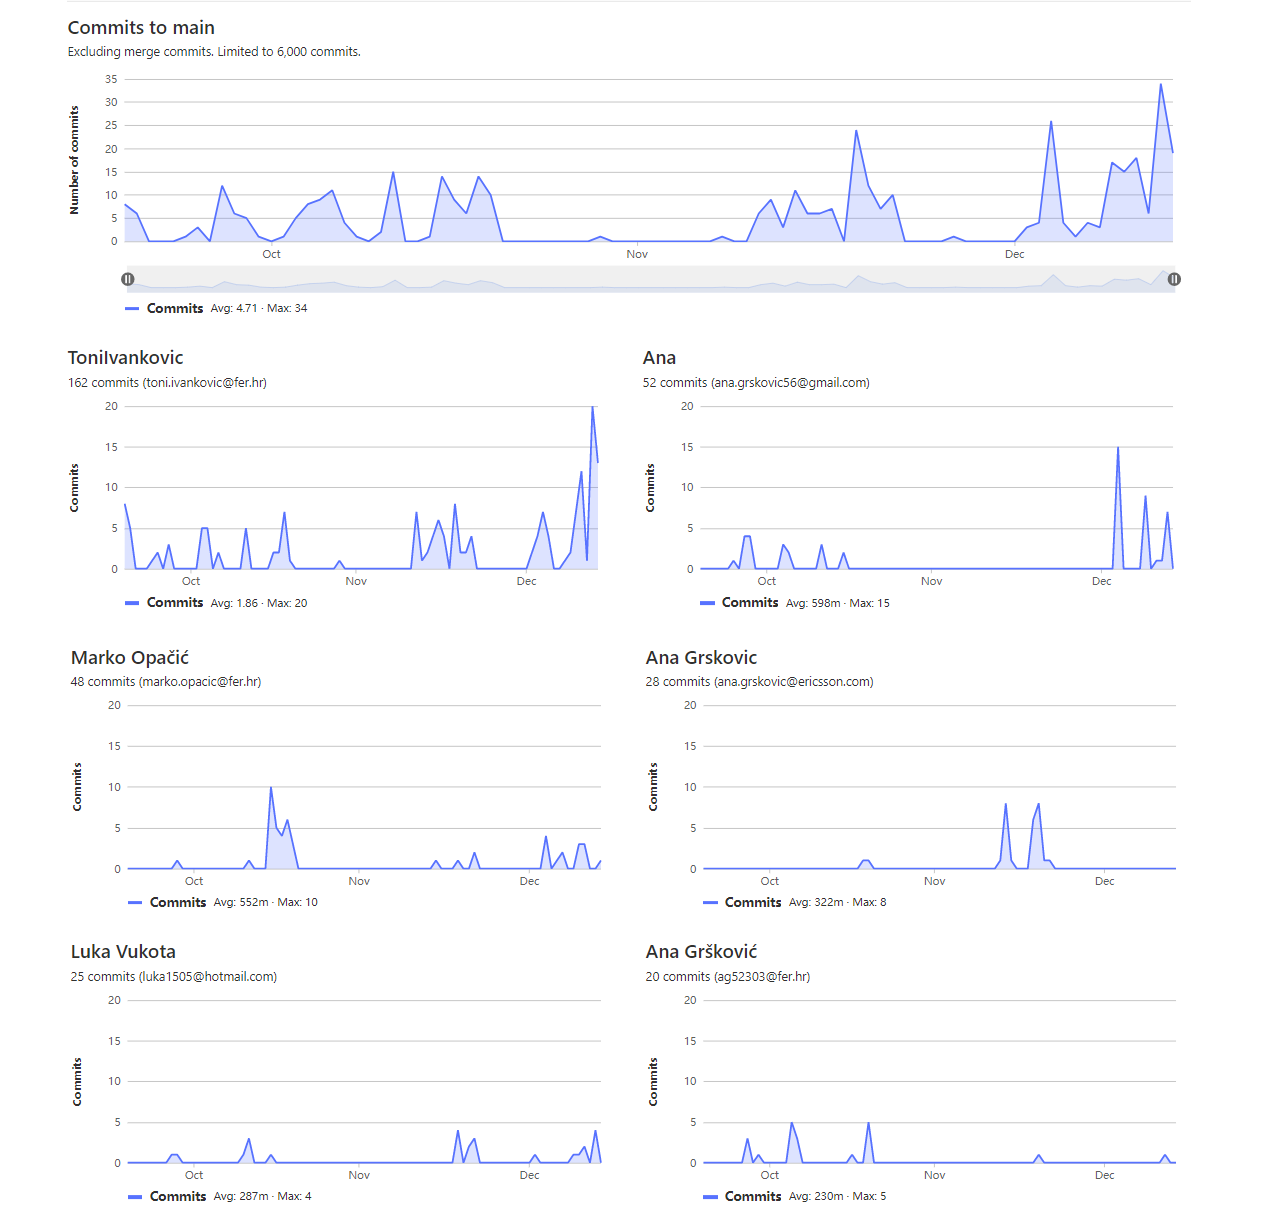
\includegraphics{slike/Graf aktivnosti.png}
    \caption{Graf aktivnosti - 1. dio}
    \label{fig:grarf_aktivnosti_1}
\end{figure}
\begin{figure}
    \centering
    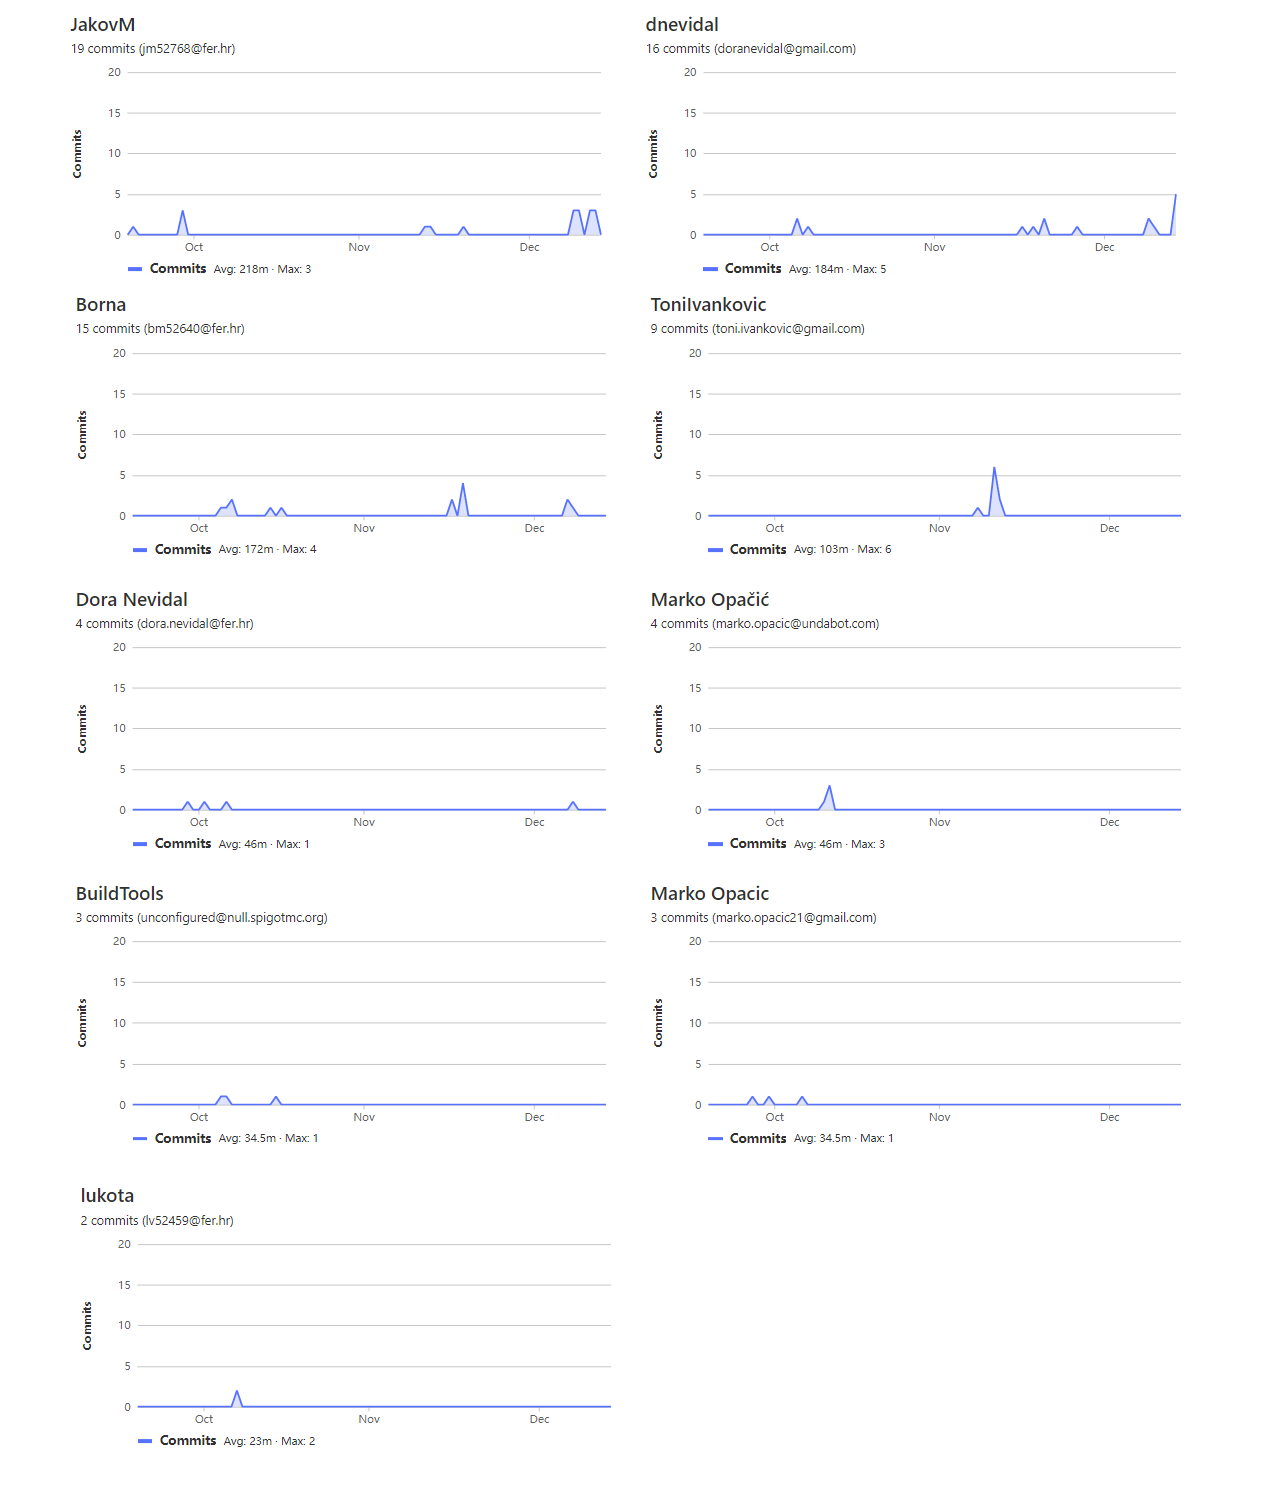
\includegraphics{slike/Graf aktivnosti - 2.png}
    \caption{Graf aktivnosti - 2. dio}
    \label{fig:grarf_aktivnosti_2}
\end{figure}
		
	


\end{document} %naredbe i tekst nakon ove naredbe ne ulaze u izgrađen dokument 


